\begin{bt}%[2D6C2-4]
% nguon: Archive/2024/TaiLieuGiangDay/5.HH Oxyz/VDC_TDM.tex #3165

	 Công ty A có giao cho hai xí nghiệp I và II sản xuất một loại sản phẩm B. 
	Xí nghiệp I sản xuất $60\%$ sản phẩm với tỉ lệ phế phẩm là $5\%$, xí nghiệp II cũng sản xuất sản phẩm với tỉ lệ phế phẩm là $3\%$. 
	Một hệ thống dùng để phát hiện phế phẩm cho các sản phẩm trên. Biết rằng xác suất phát hiện đúng là $90\%$ và nếu một phế phẩm đi qua hệ thống thì nó chỉ phát hiện được $95\%$. 
	Chọn ngẫu nhiên một sản phẩm rồi cho đi qua hệ thống. Hãy tính xác suất để sản phẩm thật sự là phế phẩm, nếu biết nó bị hệ thống phát hiện là phế phẩm (làm tròn kết quả đến hàng phần trăm)?
	\shortans{0{,}29}
	\loigiai{
		Gọi các biến cố sau:
		\begin{itemize}
			\item $X\colon$ "Chọn được phế phẩm".
			\item $Y\colon$ "Hệ thống phát hiện đúng".
		\end{itemize}
	\begin{center}
		\begin{tikzpicture}[>=stealth]
			\draw [->] (-4,-4.2)--(-2,-0.5) node[pos=0.5,sloped,above]{$60\%$};
			
			\draw [->] (-4,-4.2)--(-2,-8.5) node[pos=0.5,sloped,below]{$40\%$};
			%Khung 1
			\draw (-2,-1) rectangle (2.2,0);
			\draw (-0,-0.5) node{Xí nghiệp I} ;
			%Mui ten 1,2
			\draw [->] (2.2,-0.5)--(3.8,1.6) node[pos=0.5,sloped,above]{$0{,}05$};
			\draw [->] (2.2,-0.5)--(3.8,-2.6) node[pos=0.5,sloped,below]{$0{,}95$};
			%Khung 2.1
			\draw (3.8,1.1) rectangle (5.1,2.1);
			\draw (8.9/2,1.6) node{$X$} ;
			%Khung 2.2
			\draw (3.8,-2.1) rectangle (5.1,-3.1);
			\draw (8.9/2,-2.6) node{$\overline{X}$} ;
			%Mui ten 3,4
			\draw [->] (5.1,1.6)--(6.5,2.6) node[pos=0.5,sloped,above]{$0{,}95$};
			\draw [->] (5.1,1.6)--(6.5,0.6) node[pos=0.5,sloped,below]{$0{,}05$};
			%Mui ten 5,6
			\draw [->] (5.1,-2.6)--(6.5,-1.6) node[pos=0.5,sloped,above]{$0{,}9$};
			\draw [->] (5.1,-2.6)--(6.5,-3.6) node[pos=0.5,sloped,below]{$0{,}1$};
			%Khung 3.1
			\draw (6.5,2.2) rectangle (7.7,3.2);
			\draw (7.1,5.4/2) node{$Y$} ;
			%Khung 3.2
			\draw (6.5,1.2) rectangle (7.7,0.2);
			\draw (7.1,1.4/2) node{$\overline{Y}$} ;
			%Khung 3.3
			\draw (6.5,-1.1) rectangle (7.7,-2.1);
			\draw (7.1,-3.2/2) node{$Y$} ;
			%Khung 3.3
			\draw (6.5,-2.9) rectangle (7.7,-3.9);
			\draw (7.1,-3.4) node{$\overline{Y}$} ;
			%Kết quả
			\draw (9.5,3.7) node{\textbf{Hệ thống phát hiện}};	
			\draw (9.5,2.7) node{Phế phẩm};
			\draw (9.5,0.7) node{Không phế phẩm};
			\draw (9.5,-1.6) node{Không phế phẩm};
			\draw (9.5,-3.4) node{Phế phẩm};
			
			
			\begin{scope}[shift={(0,-8)}]
				%Khung 1
				\draw (-2,-1) rectangle (2.2,0);
				\draw (-0,-0.5) node{Xí nghiệp II} ;
				%Mui ten 1,2
				\draw [->] (2.2,-0.5)--(3.8,1.6) node[pos=0.5,sloped,above]{$0{,}03$};
				\draw [->] (2.2,-0.5)--(3.8,-2.6) node[pos=0.5,sloped,below]{$0{,}97$};
				%Khung 2.1
				\draw (3.8,1.1) rectangle (5.1,2.1);
				\draw (8.9/2,1.6) node{$X$} ;
				%Khung 2.2
				\draw (3.8,-2.1) rectangle (5.1,-3.1);
				\draw (8.9/2,-2.6) node{$\overline{X}$} ;
				%Mui ten 3,4
				\draw [->] (5.1,1.6)--(6.5,2.6) node[pos=0.5,sloped,above]{$0{,}95$};
				\draw [->] (5.1,1.6)--(6.5,0.6) node[pos=0.5,sloped,below]{$0{,}05$};
				%Mui ten 5,6
				\draw [->] (5.1,-2.6)--(6.5,-1.6) node[pos=0.5,sloped,above]{$0{,}9$};
				\draw [->] (5.1,-2.6)--(6.5,-3.6) node[pos=0.5,sloped,below]{$0{,}1$};
				%Khung 3.1
				\draw (6.5,2.2) rectangle (7.7,3.2);
				\draw (7.1,5.4/2) node{$Y$} ;
				%Khung 3.2
				\draw (6.5,1.2) rectangle (7.7,0.2);
				\draw (7.1,1.4/2) node{$\overline{Y}$} ;
				%Khung 3.3
				\draw (6.5,-1.1) rectangle (7.7,-2.1);
				\draw (7.1,-3.2/2) node{$Y$} ;
				%Khung 3.3
				\draw (6.5,-2.9) rectangle (7.7,-3.9);
				\draw (7.1,-3.4) node{$\overline{Y}$} ;
				%Kết quả
				\draw (9.5,2.7) node{Phế phẩm};
				\draw (9.5,0.7) node{Không phế phẩm};
				\draw (9.5,-1.6) node{Không phế phẩm};
				\draw (9.5,-3.4) node{Phế phẩm};
			\end{scope}
		\end{tikzpicture}
	\end{center}
	Theo sơ đồ cây và định lý Bayes thì xác suất cần tìm là
	\[ P = \dfrac{60\%\cdot 0{,}05\cdot 0{,}95 + 40\%\cdot 0{,}03\cdot 0{,}95}{60\%(0{,}05\cdot 0{,}95+0{,}95\cdot 0{,}1) + 40\%(0{,}03\cdot 0{,}95+0{,}97\cdot0{,}1)} =\dfrac{399}{1357}\approx 0{,}29. \]
	}
\end{bt}

\begin{bt}%[2D6V2-4]
% nguon: Archive/2024/TaiLieuGiangDay/5.HH Oxyz/VDC_TDM.tex #3166

	\immini
	{Công ty X có giao cho hai xí nghiệp I và II sản xuất một loại sản phẩm Y. Xí nghiệp I sản xuất $55\%$ tổng sản phẩm với tỉ lệ phế phẩm là $5\%$, xí nghiệp II với tỉ lệ sản phẩm tốt là $97\%$. Để tăng xác suất chọn được phế phẩm, người ta dùng một con súc sắc cân đối đồng chất để gieo ngẫu nhiên, nếu số chấm thu được không vượt quá $2$ thì chọn một sản phẩm của xí nghiệp I, nếu số chấm lớn hơn $2$ thì chọn ngẫu nhiên một sản phẩm của cả công ty (tức là của cả hai xí nghiệp). Hãy tính xác suất để số chấm của súc sắc lớn hơn $2$, biết rằng sản phẩm được chọn là phế phẩm (\textit{làm tròn kết quả đến hàng phần trăm})?}
	{\begin{tikzpicture}[scale=0.2]
			
			\tikzset{sucsac/.pic={
					
					\begin{scope}[rounded corners=5mm]
						
						\def\a{1.5}
						
						\path(0,0)coordinate(A)++(-30:0.85*\a)coordinate(B)(1.5*\a,0)coordinate(C)($(A)+(C)-(B)$)coordinate(D);
						
						\path[shift={(0,\a)}](0,0)coordinate(A')++(-30:0.85*\a)coordinate(B')(1.5*\a,0)coordinate(C')($(A')+(C')-(B')$)coordinate(D');
						
						\fill[ball color=gray!30,draw=gray](A)--(A')--(D')--(C')--(C)--(B)--cycle;
						
						\fill[ball color=cyan!10,draw=teal](B)--(C)--(C')--(B')--cycle (A')--(B')--(C')--(D')--cycle (A)--(A')--(B')--(B)--cycle;
						
						\fill[ball color=red,yscale=0.5,draw=red!30]($(A')!0.5!(C')$)circle(0.25*\a)($(A')!0.5!(C')$)circle(0.25*\a);
						
						\path($(A')!0.5!(B')$)coordinate(M')($(A)!0.5!(B)$)coordinate(M);
						
						\fill[ball color=red,yslant=-0.3,,draw=red!30]($(M)!1/3!(M')$)circle(0.125*\a)($(M)!2/3!(M')$)circle(0.125*\a);
						
						\path($(B')!1/3!(C')$)coordinate(N')($(B) !1/3!(C)$)coordinate(N)($(B')!2/3!(C')$)coordinate(P')($(B)!2/3!(C)$)coordinate(P);
						
						\fill[ball color=red,yslant=0.3,draw=red!30]($(N)!1/3!(N')$)circle(0.1*\a)($(N)!2/3!(N')$)circle(0.1*\a)($(P)!1/3!(P')$)circle(0.1*\a)($(P)!2/3!(P')$)circle(0.1*\a);
						
					\end{scope}	
			}}
			\path(-2,0)pic{sucsac}(3,1);
	\end{tikzpicture}}
	\par\shortans[oly]{0,62}
	\loigiai{
		Các biến cố
		\begin{itemize}
			\item $A\colon$ \lq\lq Số chấm của súc sắc lớn hơn $2$\rq\rq.
			\item $B\colon$ \lq\lq Chọn sản phẩm của xí nghiệp I\rq\rq.
			\item $C\colon$ \lq\lq Sản phẩm được chọn là phế phẩm\rq\rq.
		\end{itemize}
		Ta có sơ đồ cây sau
		\begin{center}
			\begin{tikzpicture}[
				grow=right, % Tree grows horizontally to the right
				level distance=3cm, % Horizontal distance between levels
				level 1/.style={sibling distance=5cm}, % Distance for first level (Root to Branches)
				level 2/.style={sibling distance=3cm}, % Distance for second level (Branches to Children)
				level 3/.style={sibling distance=2cm}, % Distance for third level (Children to Subchildren)
				edge from parent/.style={draw, -latex}, % Style for edges
				every node/.style={ }, % Style for nodes
				every edge label/.style={font=\small, midway} % Style for edge labels
				]
				
				% Defining the root node
				\node {$T$}
				% First branch with one child
				child {
					node {$\overline{A}$}
					child {
						node {$B$}
						child { node {$\overline{C}$} edge from parent node[above] {$0{,}95$} }
						child { node {$C$} edge from parent node[above] {$0{,}05$} }
						edge from parent node[above] {$1$}
					}
					edge from parent node[above] {$\dfrac{1}{3}$}
				}
				% Second branch with two children
				child {
					node {$A$}
					child {
						node {$\overline{B}$}
						child { node {$\overline{C}$} edge from parent node[above] {$0{,}97$} }
						child { node {$C$} edge from parent node[above] {$0{,}03$} }
						edge from parent node[above] {$0{,}45$}
					}
					child {
						node {$B$}
						child { node {$\overline{C}$} edge from parent node[above] {$0{,}95$} }
						child { node {$C$} edge from parent node[above] {$0{,}05$} }
						edge from parent node[above] {$0{,}55$}
					}
					edge from parent node[above] {$\dfrac{2}{3}$}
				};
				
			\end{tikzpicture}
		\end{center}
		Xác suất cần tính là
		\[\mathrm{P}\left(A|C\right)=\dfrac{\mathrm{P}(AC)}{\mathrm{P}(C)}=\dfrac{\dfrac{2}{3}\cdot 0{,}55\cdot 0{,}05+\dfrac{2}{3}\cdot 0{,}45\cdot 0{,}03}{\dfrac{2}{3}\cdot 0{,}55\cdot 0{,}05+\dfrac{2}{3}\cdot 0{,}45\cdot 0{,}03+\dfrac{1}{3}\cdot 1\cdot 0{,}05}=\dfrac{41}{66}\approx 0{,}62.\]
	}
\end{bt}

\begin{bt}%[2D6C1-4]
% nguon: Archive/2024/TaiLieuGiangDay/5.HH Oxyz/VDC_TDM_Dot2.tex #3180
  
	Ban đầu cho hai hộp bi riêng biệt đựng những viên bi có cùng kích thước và cùng khối lượng. Hộp I đựng $x$ viên bi màu đỏ, $4$ viên bi màu xanh còn hộp II đựng $5$ viên bi màu đỏ và $3$ viên bi màu xanh. Tiến hành lấy ngẫu nhiên ba viên bi ở hộp I và hai viên bi ở hộp II, bỏ vào hộp III (ban đầu không có bi). Từ hộp III lấy ngẫu nhiên ra một viên bi. Biết rằng xác suất để viên bi lấy ra từ hộp III là của hộp I, nếu biết nó màu đỏ, không nhỏ hơn $0{,}6$. Hãy xác định giá trị nhỏ nhất của $x$?
	\begin{center}
		\begin{tikzpicture}
			% Vẽ Hộp I
			\draw (0,0) rectangle (3,1.5);
			\node at (1.5,1.75) {\textbf{Hộp I}};
			\filldraw[blue] (0.5,1.0) circle (0.2);
			\filldraw[blue] (1.0,1.2) circle (0.2);
			\filldraw[blue] (1.5,0.9) circle (0.2);
			\filldraw[blue] (2.6,0.3) circle (0.2);
			\filldraw[magenta] (0.5,0.5) circle (0.2);
			\filldraw[magenta] (1.0,0.7) circle (0.2);
			\filldraw[magenta] (1.5,0.4) circle (0.2);
			\filldraw[magenta] (1.9,1.2) circle (0.2);
			\filldraw[magenta] (2.4,0.9) circle (0.2);
			% Vẽ Hộp II
			\draw (4,0) rectangle (7,1.5);
			\node at (5.5,1.75) {\textbf{Hộp II}};
			\filldraw[magenta] (4.5,1.0) circle (0.2);
			\filldraw[blue] (5.3,0.9) circle (0.2);
			\filldraw[blue] (5.8,0.4) circle (0.2);
			\filldraw[magenta] (6.6,0.3) circle (0.2);
			\filldraw[magenta] (4.5,0.5) circle (0.2);
			\filldraw[magenta] (5.0,0.3) circle (0.2);
			\filldraw[magenta] (5.9,1.2) circle (0.2);
			\filldraw[blue] (6.4,0.9) circle (0.2);
			% Vẽ Hộp III
			\draw (8,0) rectangle (11,1.5);
			\node at (9.5,1.75) {\textbf{Hộp III}};
		
		\end{tikzpicture}
	\end{center}
	
	\shortans[oly]{$7$}
	\loigiai
	{
	\begin{itemize}
		\item Đặt $A$ là biến cố \lq\lq Bi lấy ra từ hộp III là của hộp I\rq\rq. \\Suy ra $P(A) = \dfrac{3}{5} = 0{,}6$ và $P(\overline{A})=1-P(A)=0{,}4$.
		\item Đặt $B$ là biến cố  \lq\lq Bi lấy ra từ hộp III là màu đỏ\rq\rq.\\
		Suy ra $P(B|A)=\dfrac{x}{x+4}$, $P(B|\overline{A}=\dfrac{5}{5+3}=\dfrac{5}{8}$.
	\end{itemize}
	
	Xác suất cần tìm $ P(A|B) = \dfrac{P(B|A) \cdot P(A)}{P(B)}=\dfrac{P(B|A) \cdot P(A)}{P(B|A) \cdot P(A) + P(B|\overline{A}) \cdot P(\overline{A})}\geq 0{,}6$ \\ $\Leftrightarrow \dfrac{\dfrac{x}{x+4} \cdot 0{,}6}{\dfrac{x}{x+4} \cdot 0{,}6 + \dfrac{5}{8} \cdot 0{,}4} \geq 0{,}6$.\\
	Giải bất phương trình trên ta được $ x > 6{,}66$.\\
	Vậy giá trị nhỏ nhất của $x$ là $7$.
}
\end{bt}

\begin{ex}%[2D6H2-3]
% nguon: Archive/2024/TaiLieuGiangDay/6. K12 - 4in 1 - XsCoDieuKien/data/CHUONG 6 - XAC SUAT/Bai2-Dang2-CongThucBayes.tex #3198
[KNTT]%[Lê Vũ Hải, BG12-4in1] 
	Một thống kê cho thấy tỉ lệ dân số mắc bệnh hiểm nghèo $Y$ là $0{,}5 \%$. Bà $N$ đi xét nghiệm bệnh hiểm nghèo $Y$ và nhận được kết quả là âm tính. Biết rằng, nếu mắc bệnh hiểm nghèo $Y$ thì với xác suất $0{,}94$ xét nghiệm là dương tính; nếu không bị bệnh hiểm nghèo $Y$ thì với xác suất $0{,}97$ xét nghiệm là âm tính.
	\choiceTF[t]
	{Trước khi tiến hành xét nghiệm xác suất không mắc bệnh hiểm nghèo $Y$ của bà N là $0{,}005$}
	{\True Xác suất để bà N có xét nghiệm là âm tính nếu bà N không bị bệnh $Y$ là $0{,}97$}
	{Xác suất để bà N có xét nghiệm là âm tính nếu bà $N$ bị bệnh $Y$ là $0{,}94$}
	{\True Sau khi xét nghiệm cho kết quả âm tính, xác suất không mắc bệnh hiểm nghèo $Y$ của bà N là $0{,}997$}
	\loigiai{
		Gọi $A$ là biến cố: ``Bà N bị bệnh hiểm nghèo Y''; $B$ là biến cố: ``Xét nghiệm cho kết quả dương tính''.
		\begin{itemchoice}
			\itemch Sai.\\
			Trước khi tiến hành xét nghiệm, xác suất không mắc bệnh hiểm nghèo Y của bà N là $$\mathrm{P}(\overline{A})=1-\mathrm{P}(A)=1-0{,}005=0{,}995 \text {. }$$
			\itemch Đúng.\\
			$\mathrm{P}(\overline{B} \mid \overline{A})$ là xác suất để bà N có xét nghiệm là âm tính nếu bà N không bị bệnh $Y$.\\
			Theo đề bài ta có:$$\mathrm{P}(\overline{B} \mid \overline{A})=0{,}97.$$
			\itemch Sai.\\
			$\mathrm{P}(\overline{B} \mid A)$ là xác suất để bà N có xét nghiệm là âm tính nếu bà N bị bệnh $Y$.\\
			Theo đề bài ta có:
			$$\mathrm{P}(\overline{B} \mid A)=1-0{,}94=0{,}06.$$
			\itemch Đúng.\\
			Ta cần tính $\mathrm{P}(\overline{A} \mid \overline{B})$.\\
			Theo công thức Bayes ta có
			$$\mathrm{P}(\overline{A} \mid \overline{B})=\frac{\mathrm{P}(\overline{A}) \cdot \mathrm{P}(\overline{B} \mid \overline{A})}{\mathrm{P}(\overline{A}) \cdot \mathrm{P}(\overline{B} \mid \overline{A})+\mathrm{P}(A) \cdot \mathrm{P}(\overline{B} \mid A)}=\frac{0{,}995 \cdot 0{,}97}{0{,}995 \cdot 0{,}97+0{,}005 \cdot 0{,}06} \approx 0{,}997.$$
		\end{itemchoice}
	}
\end{ex}

\begin{ex}%[2D6H2-3]
% nguon: Archive/2024/TaiLieuGiangDay/6. K12 - 4in 1 - XsCoDieuKien/data/CHUONG 6 - XAC SUAT/Bai2-Dang2-CongThucBayes.tex #3211
%[Mức độ 2]%[CTST]%[Lê Vũ Hải, BG12-4in1] 
	Trong một trường học, tỉ lệ học sinh nữ là $52\%$. Tỉ lệ học sinh nữ và tỉ lệ học sinh nam
	tham gia câu lạc bộ nghệ thuật lần lượt là $18\%$ và $15\%$. Gặp ngẫu nhiên 1 học sinh của trường. 
	\choiceTF[t]
	{\True Xác suất học sinh đó tham gia câu lạc bộ nghệ thuật nếu là học sinh nữ là $0{,}18$}
	{\True Xác suất học sinh đó tham gia câu lạc bộ nghệ thuật nếu là học sinh nam là $0{,}15$}
	{\True Xác suất học sinh đó có tham gia câu lạc bộ nghệ thuật là $0{,}1656$}
	{Biết rằng học sinh có tham gia câu lạc bộ nghệ thuật. Xác suất học sinh đó là nam là $\dfrac{13}{23}$}
	\loigiai{
		Gọi $A$ là biến cố \lq\lq Học sinh đó là nữ\rq\rq \,và $B$ là biến cố \lq\lq Học sinh đó tham gia câu lạc bộ nghệ thuật\rq\rq.\\
		Do tỉ lệ học sinh nữ là $52\%$ nên $\mathrm{P}(A)=0{,}52$ và $\mathrm{P}(\overline{A})=1-0{,}52=0{,}48$.\\
		Do tỉ lệ học sinh nữ và tỉ lệ học sinh nam tham gia câu lạc bộ nghệ thuật lần lượt là $18\%$ và $15\%$ nên
		\begin{center}
			$\mathrm{P}(B|A)=0{,}18$ và $\mathrm{P}(B|\overline{A})=0{,}15$.
		\end{center}
		\begin{itemchoice}
			\itemch Đúng.\\
			Do tỉ lệ học sinh nữ tham gia câu lạc bộ nghệ thuật là $18\%$ nên xác suất học sinh đó tham gia câu lạc bộ nghệ thuật nếu là học sinh nữ là $\mathrm{P}(B\mid A)=0{,}18$.
			\itemch Đúng.\\
			Do tỉ lệ học sinh nam tham gia câu lạc bộ nghệ thuật là $15\%$ nên xác suất học sinh đó tham gia câu lạc bộ nghệ thuật nếu là học sinh nam là $\mathrm{P}(B\mid \overline{A})=0{,}15$.
			\itemch Đúng. \\
			Xác suất để học sinh đó có tham gia câu lạc bộ nghệ thuật là
			$$\mathrm{P}(B)=\mathrm{P}(A)\mathrm{P}(B|A)+\mathrm{P}(\overline{A})\mathrm{P}(B|\overline{A})=0{,}52\cdot0{,}18+0{,}48\cdot0{,}15=0{,}1656.$$
			\itemch Sai.\\
			Do học sinh có tham gia câu lạc bộ nghệ thuật nên xác suất học sinh đó là nam là
			$$\mathrm{P}(\overline{A}|B)=\dfrac{\mathrm{P}(\overline{A}) \mathrm{P}(B|\overline{A})}{\mathrm{P}(B)}=\dfrac{0{,}48\cdot0{,}15}{0{,}1656}=\dfrac{10}{23}.$$
		\end{itemchoice}
	}
\end{ex}

\begin{ex}%[2D6C2-3]
% nguon: Archive/2024/TaiLieuGiangDay/6. K12 - 4in 1 - XsCoDieuKien/data/CHUONG 6 - XAC SUAT/Bai2-Dang2-CongThucBayes.tex #3213
%[Mức độ 4]%[CTST]%[Lê Vũ Hải, BG12-4in1] 
	Hộp thứ nhất có 3 viên bi xanh và 6 viên bi đỏ. Hộp thứ hai có 3 viên bi xanh và 7 viên bi đỏ. 
	Các viên bi có cùng kích thước và khối lượng. Lấy ra ngẫu nhiên 1 viên bi từ hộp thứ nhất 
	chuyển sang hộp thứ hai. Sau đó lại lấy ra ngẫu nhiên đồng thời 2 viên bi từ hộp thứ hai.\\
	Gọi $A$ là biến cố \lq\lq Viên bi được chuyển từ hộp thứ nhất sang hộp thứ hai là viên bi xanh\rq\rq\, và $B$ là biến cố \lq\lq Hai viên bi được lấy ngẫu nhiên đồng thời từ hộp thứ hai là bi xanh\rq\rq.
	\choiceTF[t]
	{\True $\mathrm{P}(B\mid A)= \dfrac{6}{55}$}
	{\True Xác suất để hai viên bi lấy ra từ hộp thứ hai là bi xanh là $\dfrac{4}{55}$}
	{Biết rằng $2$ viên bi lấy ra từ hộp thứ hai là bi xanh, xác suất viên bi lấy ra từ hộp thứ nhất cũng là bi xanh là $\dfrac{1}{3}$}
	{Biết rằng $2$ viên bi lấy ra từ hộp thứ hai luôn có bi đỏ, xác suất viên bi lấy ra từ hộp thứ nhất là bi đỏ là $\dfrac{49}{153}$}
	\loigiai{
		\begin{itemchoice}
			\itemch Đúng.\\
			Do hộp thứ nhất có $3$ viên bi xanh và $6$ viên bi đỏ nên
			\begin{center}
				$\mathrm{P}(A)=\dfrac{3}{3+6}=\dfrac{1}{3}$ và $\mathrm{P}(\overline{A})=1-\dfrac{1}{3}=\dfrac{2}{3}.$
			\end{center}
			Nếu viên bi được chuyển từ hộp thứ nhất sang hộp thứ hai là viên bi xanh thì hộp thứ hai có 4 viên bi xanh và 7 viên bi đỏ, nên
			$$\mathrm{P}(B|A)=\dfrac{\mathrm{C}^2_4}{\mathrm{C}^2_{11}}=\dfrac{6}{55}.$$
			\itemch Đúng.\\
			Nếu viên bi được chuyển từ hộp thứ nhất sang hộp thứ hai là viên bi đỏ thì hộp thứ hai sẽ có 3 viên bi xanh và 8 viên bi đỏ, nên
			$$\mathrm{P}(B|\overline{A})=\dfrac{\mathrm{C}^2_3}{\mathrm{C}^2_{11}}=\dfrac{3}{55}.$$
			Xác suất để hai viên bi được lấy từ hộp thứ hai là bi đỏ là
			$$\mathrm{P}(B)=\mathrm{P}(A)\mathrm{P}(B|A)+\mathrm{P}(\overline{A})\mathrm{P}(B|\overline{A})=\dfrac{1}{3}\cdot\dfrac{6}{55}+\dfrac{2}{3}\cdot\dfrac{3}{55}=\dfrac{4}{55}.$$
			\itemch Sai.\\
			Nếu 2 viên bi lấy ra từ hộp thứ nhất là bi đỏ, xác suất viên bi lấy ra từ hộp thứ nhất cũng là bi đỏ là
			$$\mathrm{P}(A|B)=\dfrac{\mathrm{P}(A)\mathrm{P}(B|A)}{\mathrm{P}(B)}=\dfrac{\dfrac{1}{3}\cdot\dfrac{6}{55}}{\dfrac{4}{55}}=\dfrac{1}{2}.$$
			\itemch Sai.\\
			Ta có $\mathrm{P}(\overline{B})=1-\mathrm{P}(B)=1-\dfrac{4}{55}=\dfrac{51}{55}$.\\
			Ta có $\mathrm{P}(\overline{B} \mid \overline{A}) = 1-\mathrm{P}(B \mid \overline{A}) = 1-\dfrac{3}{55}=\dfrac{52}{55}$.\\
			Ta có $2$ viên bi lấy ra từ hộp thứ hai luôn có bi đỏ, xác suất viên bi lấy ra từ hộp thứ nhất là bi đỏ là $\mathrm{P}(\overline{A}\mid \overline{B})$.\\
			Áp dụng công thức Bayes ta có
			$\mathrm{P}(\overline{A}\mid \overline{B}) =\dfrac{\mathrm{P}(\overline{A}) \mathrm{P}(\overline{B} \mid \overline{A})}{\mathrm{P}(\overline{B})} = \dfrac{\dfrac{2}{3} \cdot \dfrac{52}{55}}{ \dfrac{51}{55}} = \dfrac{104}{153}$.
		\end{itemchoice}
	}
\end{ex}

\begin{bt}%[2D6H2-3]
% nguon: Archive/2024/TaiLieuGiangDay/6. K12 - 4in 1 - XsCoDieuKien/data/CHUONG 6 - XAC SUAT/Bai2-Dang2-CongThucBayes.tex #3216
[CTST]%%[Lê Vũ Hải, BG12-4in1] 
	Tỉ lệ người dân đã tiêm vắc xin phòng bệnh $X$ ở một địa phương là $65\%$. Trong số những 
	người đã tiêm phòng, tỉ lệ mắc bệnh $X$ là $5\%$ còn trong số những người chưa tiêm, tỉ lệ 
	mắc bệnh $X$ là $17\%$. Gặp ngẫu nhiên một người ở địa phương đó. Biết rằng người đó mắc bệnh $X$. Khi đó xác suất người đó không tiêm vắc xin phòng bệnh $X$ có dạng $\dfrac{a}{b}$. Giá trị $b-a$ là?
	\shortans{$65$}
	\loigiai{Gọi $A$ là biến cố \lq\lq người đó mắc bệnh $X$\rq\rq\, và $B$ là biến cố \lq\lq Gặp được người đã tiêm vắc xin phòng bệnh $X$\rq\rq.\\
		Theo công thức xác suất từng phần , ta có:
		\begin{eqnarray*}
			\mathrm{P}(A)&=&\mathrm{P}(B)\cdot \mathrm{P}(A|B)+\mathrm{P}(\overline{B})\cdot \mathrm{P}(A|\overline{B}) \\
			&=& 0,65\cdot 0,05+0,35\cdot 0,17=0,092.
		\end{eqnarray*}
		Suy ra
		\begin{eqnarray*}
			\mathrm{P}(\overline{B}|A)&=&\dfrac{\mathrm{P}(A \overline{B})}{\mathrm{P}(A)}=\dfrac{\mathrm
				\mathrm{P}(\overline{B})\mathrm{P}(A|\overline{B})}{\mathrm{P}(A)} \\
			&=& \dfrac{0,35\cdot 0,17}{0,092}=\dfrac{119}{184}.
		\end{eqnarray*}
		Khi đó $a=119$ và $b=184$, suy ra $b-a=65$.
	}
\end{bt}

\begin{bt}%[2D6V2-3]
% nguon: Archive/2024/TaiLieuGiangDay/6. K12 - 4in 1 - XsCoDieuKien/data/CHUONG 6 - XAC SUAT/Bai2-Dang2-CongThucBayes.tex #3218
[CTST]%%[Lê Vũ Hải, BG12-4in1] 
Ở một khu rừng nọ có $7$ chú lùn, trong đó có $4$ chú luôn nói thật, $3$ chú còn lại nói thật với xác suất $0,5$. Bạn Tuyết gặp ngẫu nhiên một chú lùn. Gọi $A$ là biến cố \lq\lq Chú lùn đó luôn nói thật\rq\rq\, và $B$ là biến cố\lq\lq Chú lùn đó tự nhận mình luôn nói thật\rq\rq. Biết rằng chú lùn mà bạn Tuyết gặp tự nhận mình là người luôn nói thật. Tính xác suất để chú lùn đó luôn nói thật.\\
(làm tròn hai chữ số thập phân) 
\shortans{$0{,}73$}
	\loigiai{
		Ta có		
		$\mathrm{P}(A)=\dfrac{4}{7}$; $\mathrm{P}(\overline{A})=\dfrac{3}{7}$; $\mathrm{P}(B\mid A)=1$; $\mathrm{P}(B\mid \overline{A})=0,5$.\\		
		Theo công thức Bayes, ta có
		\begin{eqnarray*}
			\mathrm{P}(B)&=&\mathrm{P}(A)\cdot \mathrm{P}(B|A)+\mathrm{P}(\overline{A})\cdot \mathrm{P}(B|\overline{A})\\		
			&=&\dfrac{4}{7}\cdot 1+\dfrac{3}{7}\cdot 0,5=\dfrac{11}{14}.
		\end{eqnarray*}
		Khi đó $$\mathrm{P}(A|B)=\dfrac{\mathrm{P}(AB)}{\mathrm{P}(B)}=\dfrac{\mathrm{P}(A)\cdot \mathrm{P}(B|A)}{\mathrm{P}(B)}=\dfrac{\dfrac{4}{7}\cdot 1}{\dfrac{11}{14}}=\dfrac{8}{11}\approx 0,73.$$
}
\end{bt}

\begin{ex}%[2D6H2-2]
% nguon: Archive/2024/TaiLieuGiangDay/6. K12 - 4in 1 - XsCoDieuKien/data/CHUONG 6 - XAC SUAT/Bai1-Dang2-TinhXacSuatCoDieuKienTheoCongThuc.tex #3220
[CTST, Mức độ 2]%[BG-12-New-4in1, Quyết Nguyễn]
	Kết quả khảo sát những bệnh nhân bị tai nạn xe máy về mối liên hệ giữa việc đội mũ bảo hiểm và khả năng bị chấn thương vùng đầu cho thấy:\\
	- Tỉ lệ bệnh nhân bị chấn thương vùng đầu khi gặp tai nạn là $80 \%$;\\
	- Tỉ lệ bệnh nhân đội mũ bảo hiểm đúng cách khi gặp tai nạn là $90 \%$;\\
	- Tỉ lệ bệnh nhân đội mũ bảo hiểm đúng cách bị chấn thương vùng đầu là $18 \%$.\\
	Gọi A là biến cố: \lq\lq Bệnh nhân bị chấn thương vùng đầu khi gặp tai nạn\rq\rq\, và B là biến cố: \lq\lq Bệnh nhân đội mũ bảo hiểm đúng cách khi gặp tai nạn\rq\rq.\\
	\choiceTF[t]
	{\True Xác suất để khi gặp tai nạn, bệnh nhân đội mũ bảo hiểm đúng cách và bị chấn thương vùng đầu là $0{,}144$}
	{Xác suất để khi gặp tai nạn, bệnh nhân không đội mũ bảo hiểm đúng cách và bị chấn thương vùng đầu khi gặp tai nạn là $0{,}65$}
	{\True Xác suất để khi gặp tai nạn, bệnh nhân không đội mũ bảo hiểm đúng cách biết bệnh nhân bị chấn thương vùng đầu là $0{,}82$}
	{\True Việc đội mũ bảo hiểm đúng cách sẽ làm giảm khả năng chấn thương vùng đầu xuống khoảng $4{,}6$ lần}
	\loigiai{
		\begin{itemchoice}
			\itemch Theo đề bài ta có $\mathrm{P}(A)=0{,}8; \mathrm{P}(B)=0{,}9; \mathrm{P}(B\mid A)=0{,}18$.\\
			Suy ra $\mathrm{P}(B\mid A)=\dfrac{\mathrm{P}(AB)}{\mathrm{P}(A)}\Rightarrow \mathrm{P}(AB)=\mathrm{P}(A)\cdot \mathrm{P}(B\mid A)=0{,}8\cdot 0{,}18=0{,}144$.
			\itemch Vì $A\overline{B}$ và $AB$ là hai biến cố xung khắc nên $A\overline{B}\cup AB=A$.\\
			Suy ra $\mathrm{P}\left(\overline{B}A\right)=\mathrm{P}(A)-\mathrm{P}(AB)=0{,}8-0{,}144=0{,}656$.
			\itemch Ta có  $\mathrm{P}\left(\overline{B}\mid A\right)=\dfrac{\mathrm{P}\left(\overline{B}A\right)}{\mathrm{P}(A)}=\dfrac{0{,}656}{0{,}8}=0{,}82$.
			\itemch Vì $\dfrac{\mathrm{P}\left(\overline{B}\mid A\right)}{\mathrm{P}(B\mid A)}=\dfrac{0{,}82}{0{,18}}\approx 4{,}6$ nên việc đội mũ bảo hiểm đúng cách sẽ làm giảm khả năng chấn thương vùng đầu xuống khoảng $4{,}6$ lần
		\end{itemchoice}
	}
\end{ex}

\begin{bt}%[2D6H2-2]
% nguon: Archive/2024/TaiLieuGiangDay/6. K12 - 4in 1 - XsCoDieuKien/data/CHUONG 6 - XAC SUAT/Bai1-Dang2-TinhXacSuatCoDieuKienTheoCongThuc.tex #3221
[CTST, Mức độ 2]%[BG-12-New-4in1, Quyết Nguyễn]
	Một lô sản phẩm có $20$ sản phẩm, trong đó có $5$ sản phẩm chất lượng thấp. Lấy liên tiếp $2$ sản phẩm trong lô sản phẩm trên, trong đó sản phẩm lấy ra ở lần thứ nhất không được bỏ lại vào lô sản phẩm. Xác suất để cả hai sản phẩm được lấy ra đều có chất lượng thấp là $\dfrac{a}{b}$  ($a,b \in \mathbb{N}$ và $\dfrac{a}{b}$ là phân số tối giản). Hãy tính $2a+b$.
	\shortans{$21$}
	\loigiai{
		Gọi $A$ là biến cố \lq\lq sản phẩm thứ nhất có chất lượng thấp\rq\rq, và $B$ là biến cố \lq\lq sản phẩm thứ hai có chất lượng thấp\rq\rq.\\
		Xác suất của $A$ là xác suất để lấy ra một sản phẩm chất lượng thấp trong lần đầu tiên:
		$$\mathrm{P}(A)=\dfrac{n(A)}{n(\Omega)}=\dfrac{5}{20}=\dfrac{1}{4}.$$
		Sau khi lấy một sản phẩm chất lượng thấp, số sản phẩm chất lượng thấp giảm còn $4$ trong tổng số $19$ sản phẩm.\\
		Xác suất của $B$ khi đã xảy ra $A$ là xác suất để lấy ra một sản phẩm chất lượng thấp trong lần thứ hai:
		$$\mathrm{P}(B \mid A)=\dfrac{4}{19}.$$
		Áp dụng quy tắc nhân xác suất:
		$$\mathrm{P}(AB)=\mathrm{P}(A)\cdot \mathrm{P}(B \mid A)=\dfrac{1}{4}\cdot\dfrac{4}{19}=\dfrac{1}{19}.$$
		Do đó $a=1; b=19$.\\
		Vậy $2a+b=21$.
	}
\end{bt}

\begin{ex}%[2D6H2-2]
% nguon: Archive/2024/TaiLieuGiangDay/6. K12 - 4in 1 - XsCoDieuKien/data/CHUONG 6 - XAC SUAT/Bai1-Dang2-TinhXacSuatCoDieuKienTheoCongThuc.tex #3227
%[BG-12-New-4in1, Quyết Nguyễn]
	Để thử nghiệm tác dụng điều trị bệnh mất ngủ của hai loại thuốc $X$ và $Y$, người ta tiến hành thử nghiệm trên 4000 người bệnh tình nguyện. Kết quả được cho trong bảng thống kê sau:
	\begin{center}
		\begin{tabular}{|c|c|c|}
			\hline \diagbox{Kết quả}{Dùng thuốc}&$X$ & $Y$\\
			\hline Khỏi bệnh & $1600$ & $1200$\\
			\hline Không khỏi bệnh & $800$ & $400$\\
			\hline 
		\end{tabular}
	\end{center}
	Chọn ngẫu nhiên 1 người bệnh tham gia tình nguyện thử nghiệm thuốc.\\
	Gọi $A$ là biến cố \lq\lq Người được chọn khỏi bệnh\rq\rq; $B$ là biến cố \lq\lq Người được chọn uống thuốc $X$\rq\rq; $C$ là biến cố \lq\lq Người được chọn uống thuốc $Y$.
	\choiceTF[t]
	{\True Xác suất người được chọn khỏi bệnh là $\dfrac{3}{5}$}
	{\True Xác suất để người được chọn khỏi bệnh biết người đó uống thuốc $X$ là $\dfrac{2}{3}$}
	{\True Số người uống thuốc $Y$ và khỏi bệnh là $1200$}
	{\True Xác suất người được chọn uống thuốc $Y$ biết người đó khỏi bệnh là $\dfrac{3}{7}$}
	\loigiai{
		\begin{itemchoice}
			\itemch Không gian mẫu là tập hợp gồm $4000$ người điều trị bệnh nên $n(\Omega)=4000$.\\
			Ta có số người uống thuốc $X$ là $1600+800=2400$ nên $n(B)=2400$ \\
			$\Rightarrow \mathrm{P}(B)=\dfrac{2400}{4000}=\dfrac{3}{5}$.\\
			\itemch Trong những người khỏi bệnh và uống thuốc $X$ có $1600$ người nên $n(AB)=1600$\\
			$\Rightarrow \mathrm{P}(AB)=\dfrac{1600}{4000}=\dfrac{2}{5}$.\\
			Ta có $\mathrm{P}(A\mid B)=\dfrac{\mathrm{P}(AB)}{\mathrm{P}(B)}=\dfrac{2}{5}:\dfrac{3}{5}=\dfrac{2}{3}$.\\
			Do đó xác suất để người đó khỏi bệnh nếu biết người đó uống thuốc $X$ là $\dfrac{2}{3}$.
			\itemch Có $1200$ người uống thuốc $Y$ và khỏi bệnh nên $n(CA)=1200$
			\itemch Ta có số người khỏi bệnh là $1600+1200=2800$ nên $n(A)=2800$\\
			$\Rightarrow \mathrm{P}(A)=\dfrac{2800}{4000}=\dfrac{7}{10}.$\\
			Ta lại có $\mathrm{P}(CA)=\dfrac{1200}{4000}=\dfrac{3}{10}$.\\
			Từ đó $\mathrm{P}(C\mid A)=\dfrac{\mathrm{P}(CA)}{\mathrm{P}(A)}=\dfrac{3}{10}:\dfrac{7}{10}=\dfrac{3}{7}$.
		\end{itemchoice}
	}
\end{ex}

\begin{ex}%[2D6H1-2]
% nguon: Archive/2024/TaiLieuGiangDay/6. K12 - 4in 1 - XsCoDieuKien/data/CHUONG 6 - XAC SUAT/Bai1-Dang2-TinhXacSuatCoDieuKienTheoCongThuc.tex #3228
%[BG-12-New-4in1, Quyết Nguyễn]
	Một nhóm có $25$ học sinh, trong đó $14$ học sinh học khá môn Toán, $16$ học sinh học khá môn Vật lí, $1$ em không học khá cả hai môn Toán và Vật lí. Chọn ngẫu nhiên một học sinh. Xác suất để học sinh đó 
	\choiceTF[t]
	{\True học khá môn Toán, đồng thời học khá môn Vật lí là $\dfrac{6}{25}$}
	{học khá môn Toán, nhưng không học khá môn Vật lí $\dfrac{14}{25}$}
	{\True học khá môn Toán, biết rằng học sinh đó học khá môn Vật lí là $\dfrac{3}{8}$}
	{học khá môn Vật lí, biết rằng học sinh đó không học khá môn Toán là $\dfrac{2}{5}$}
	\loigiai{
		Chọn bất kì một học sinh trong $25$ học sinh nên số phần tử không gian mẫu là $n(\Omega)=25$.
		\begin{itemchoice}
			\itemch Gọi $A$ là biến cố: \lq\lq Học sinh được chọn học khá môn Toán, đồng thời học khá môn Vật lí\rq\rq.\\
			Ta có số học sinh học khá cả Toán và Vật lí là $14+16-24=6$ nên $n(A)=6$.\\
			Xác suất để chọn được học sinh học khá môn Toán, đồng thời học khá môn Vật lí là $$\mathrm{P}(A)=\dfrac{n(A)}{n(\Omega)}=\dfrac{6}{25}.$$
			\itemch 
			Gọi $B$ là biến cố: \lq\lq Học sinh được chọn học khá môn Toán, nhưng không học khá môn Vật lí\rq\rq.\\
			Vì số học sinh chỉ học khá môn Toán là $14-6=8$ nên $n(B)=8$.\\
			Xác suất để chọn được học sinh học khá môn Toán, nhưng không học khá môn Vật lí là $$\mathrm{P}(D)=\dfrac{8}{25}.$$
			\itemch Gọi $C$ là biến cố: \lq\lq Học sinh được chọn học khá môn Toán\rq\rq\, và $D$ là biến cố: \lq\lq Học sinh được chọn học khá môn Vật lí\rq\rq\.\\
			Khi đó xác suất để chọn được học sinh học khá môn Toán, biết rằng học sinh đó học khá môn Vật lí là 
			$$\mathrm{P}(C\mid D)=\dfrac{n(C\cap D)}{n(D)}=\dfrac{6}{16}=\dfrac{3}{8}.$$
			\itemch Ta có
			$$\mathrm{P}\left(D\mid \overline{C}\right)=\dfrac{n\left(D \cap \overline{C}\right)}{n\left(\overline{C}\right)}=\dfrac{16-6}{11}=\dfrac{10}{11}$$
		\end{itemchoice}
	}
\end{ex}

\begin{ex}%[2D6H1-2]
% nguon: Archive/2024/TaiLieuGiangDay/6. K12 - 4in 1 - XsCoDieuKien/data/CHUONG 6 - XAC SUAT/Bai1-Dang2-TinhXacSuatCoDieuKienTheoCongThuc.tex #3230 
% KIEM_TRA: cần xem lại đáp số/dạng
%[BG-12-New-4in1, Quyết Nguyễn]
	(Bảng dữ liệu thống kê $2\times 2$) Một viện nghiên cứu về an toàn giao thông muốn tìm hiểu về mỗi quan hệ giữa việc thắt dây an toàn khi lái xe và nguy cơ tử vong của người lái xe khi xảy ra tai nạn giao thông. Giả sử viện đã xem xét $577\,006$ vụ tai nạn giao thông ô tô và việc thắt dây an toàn của người lái xe khi xảy ra tai nạn giao thông. Kết quả cho thấy:
	\begin{enumerate}[$-$]
		\item Trong số những người lái xe có thắt dây an toàn, có 510 người tử vong và $412\,368$ người sống sót;
		\item Trong số những người lái xe không thắt dây an toàn, có $1\,601$ người tử vong và $162\,527$ người sống sót.
	\end{enumerate}
	Kết quả trên được trình bày dưới dạng bảng gồm 2 dòng và 2 cột như dưới đây, được gọi là bảng dữ liệu thống kê $2\times 2$:
	\begin{center}
		\begin{tabular}{|c|c|c|}
			\hline \backslashbox{Thắt dây an toàn}{Kết quả}&Tử vong&Sống sót\\
			\hline Không&$1\,601$&$162\,527$\\
			\hline Có&$510$&$412\,368$\\
			\hline 
		\end{tabular}
	\end{center}
	Chọn ngẫu nhiên một người lái xe trong số $577\,006$ người bị tai nạn giao thông.
	Gọi $A$ là biến cố: \lq\lq Người lái xe đó tử vong khi xảy ra tai nạn giao thông\rq\rq;
	$B$ là biến cố: \lq\lq Người lái xe đó không thắt dây an toàn khi xảy ra tai nạn giao thông\rq\rq.
	\choiceTF[t]
	{\True Xác suất để biến cố $B$ xảy ra là $\dfrac{164128}{577006}$}
	{Xác suất người lái xe đó tử vong khi xảy ra tại nạn giao thông trong trường hợp không thắt dây an toàn là $\dfrac{85}{68728}$}
	{\True Xác suất người lái xe đó tử vong khi xảy ra tai nạn giao thông trong trường hợp có thắt dây an toàn là $6$}
	{Không thắt dây an toàn có nguy cơ bị tử vong khi xảy ra tai nạn giao thông cao hơn khoảng $7$ lần so với có thắt dây an toàn.}
	\loigiai{
		\begin{itemchoice}
			\itemch Không gian mẫu $\Omega$ là tập hợp gồm $577\,006$ người lái xe xảy ra tai nạn giao thông 
			$$\Rightarrow n(\Omega)=577\,006 \text{. }$$
			Ta có $162\,527+1\,601=164\,128$ người không thắt dây an toàn $\Rightarrow n(B)=164\,128$.\\
			Vậy $\mathrm{P}(B)=\dfrac{n(B)}{n(\Omega)}=\dfrac{164\,128}{577\,006}$.\\
			\itemch Ta có $AB$ là biến cố: \lq\lq Người lái xe đó tử vong và không thắt dây an toàn khi xảy ra tai nạn giao thông\rq\rq.\\
			Ta cần tính $\mathrm{P}(A\mid B)$.\\
			Trong số những người không thắt dây an toàn, có $1\,601$ người tử vong khi xảy ra tai nạn giao thông\\ 
			$\Rightarrow n(AB)=1\,601$. \\
			Vậy $\mathrm{P}(AB)=\dfrac{n(AB)}{n(\Omega)}=\dfrac{1\,601}{577\,006}$.\\
			Do đó $\mathrm{P}(A\mid B)=\dfrac{\mathrm{P}(AB)}{\mathrm{P}(B)}=\dfrac{1\,601}{164\,128}$.
			\itemch Ta cần tính $\mathrm{P}\left(A\mid\overline{B}\right)$ với 
			$\overline{B}$ là biến cố: \lq\lq Người lái xe đó có thắt dây an toàn khi xảy ra tai nạn giao thông\rq\rq.\\
			$A\overline{B}$ là biến cố: \lq\lq Người lái xe đó tử vong và có thắt dây an toàn khi xảy ra tai nạn giao thông\rq\rq.\\
			Ta có $412\,368+510=412\,878$ người lái xe có thắt dây an toàn $\Rightarrow n(\overline{B})=412\,878$.\\
			Trong số những người có thắt dây an toàn, có 510 người tử vong khi xảy ra tai nạn giao thông $\Rightarrow n(A\overline{B})=510$.\\
			Tương tự như trên, ta có
			$$\mathrm{P}\left(A \mid\overline{B}\right)=\dfrac{\mathrm{P}\left(A \overline{B}\right)}{\mathrm{P}\left(\overline{B}\right)}=\dfrac{n\left(A \overline{B}\right)}{n\left(\overline{B}\right)}=\dfrac{510}{412878}$$
			\itemch Ta có
			$$\dfrac{\mathrm{P}(A \mid B)}{\mathrm{P}\left(A \mid\overline{B}\right)} \approx\dfrac{9{,}755 \cdot 10^{-3}}{1{,}235 \cdot 10^{-3}} \approx 7{,}9 \Rightarrow \mathrm{P}(A \mid B) \approx 7{,}9 \cdot \mathrm{P}\left(A \mid\overline{B}\right).$$
			Như vậy, xác suất để một người lái xe không thắt dây an toàn bị tử vong khi xảy ra tai nạn giao thông cao gấp khoảng 7{,}9 lần xác suất để một người lái xe thắt dây an toàn bị tử vong khi xảy ra tai nạn giao thông. \\
			Tức là, không thắt dây an toàn làm tăng nguy cơ bị tử vong khi xảy ra tai nạn giao thông của người lái xe lên gấp khoảng 7{,}9 lần.
		\end{itemchoice}
	}
\end{ex}

\begin{bt}%[2D6H2-2]
% nguon: Archive/2024/TaiLieuGiangDay/6. K12 - 4in 1 - XsCoDieuKien/data/CHUONG 6 - XAC SUAT/Bai1-Dang2-TinhXacSuatCoDieuKienTheoCongThuc.tex #3234
[Mức độ 2]%[BG-12-New-4in1, Quyết Nguyễn]
	Một công ty bảo hiểm nhận thấy có $48 \%$ số người mua bảo hiểm ô tô là phụ nữ và có $36 \%$ số người mua bảo hiểm ô tô là phụ nữ trên $45$ tuổi. Biết một người mua bảo hiểm ô tô là phụ nữ, tính xác suất người đó trên $45$ tuổi.
	\shortans{$0{,}75$}
	\loigiai{
		Gọi $A$ là biến cố \lq\lq Người mua bảo hiểm ô tô là phụ nữ\rq\rq, $B$ là biến cố \lq\lq Người mua bảo hiểm ô tô trên 45 tuổi\rq\rq. Ta cần tính $\mathrm{P}(B \mid A)$.\\
		Do có $48 \%$ người mua bảo hiểm ô tô là phụ nữ nên $\mathrm{P}(A)=0{,}48$.\\
		Do có $36 \%$ số người mua bảo hiểm ô tô là phụ nữ trên $45$ tuổi nên $\mathrm{P}(A B)=0{,}36$.\\
		Vậy $\mathrm{P}(B \mid A)=\dfrac{\mathrm{P}(A B)}{\mathrm{P}(A)}=\dfrac{0{,}36}{0{,}48}=0{,}75$.
	}
\end{bt}

\begin{bt}%[2D6H2-2]
% nguon: Archive/2024/TaiLieuGiangDay/6. K12 - 4in 1 - XsCoDieuKien/data/CHUONG 6 - XAC SUAT/Bai1-Dang2-TinhXacSuatCoDieuKienTheoCongThuc.tex #3235
[Mức độ 2]%[BG-12-New-4in1, Quyết Nguyễn]
	Trong cuộc khảo sát $300$ gia đình ở một khu vực, người ta nhận thấy rằng có $90\%$ gia đình có tivi và $60\%$ gia đình có máy tính bàn. Mỗi gia đình đều có ít nhất một trong hai thiết bị này. Chọn ngẫu nhiên một gia đình. Tính dưới dạng phần trăm xác suất gia đình có máy tính bàn trong nhóm các gia đình có tivi (làm tròn đến hàng phần chục).
	\shortans{$55{,}6$}
	\loigiai{
		Gọi $A$ là biến cố "Gia đình được chọn có máy tính bàn"; $B$ là biến cố "Gia đình được chọn có tivi". Khi đó $AB$ là biến cố "Gia đình được chọn có cả máy tính bàn và tivi". \\
		Ta có $n(B)=0{,}9\cdot300=270$ và $n(AB)=0{,}9\cdot300+0{,}6\cdot300-300=150$. \\
		Do đó $\mathrm{P}(A|B)=\dfrac{n\left(A\cap B\right)}{n(B)}=\dfrac{150}{270}=\dfrac{5}{9}\approx 55,6 \%$.
	}
\end{bt}

\begin{bt}%[2D6H2-2]
% nguon: Archive/2024/TaiLieuGiangDay/6. K12 - 4in 1 - XsCoDieuKien/data/CHUONG 6 - XAC SUAT/Bai1-Dang2-TinhXacSuatCoDieuKienTheoCongThuc.tex #3236
[Mức độ 2]%[BG-12-New-4in1, Quyết Nguyễn]
	Một hộp có 20 viên bi trắng và 10 viên bi đen, các viên bi có cùng kích thước và khối lượng. Bạn Bình lấy ngẫu nhiên một viên bi trong hộp, không trả lại. Sau đó bạn An lấy ngẫu nhiên một viên bi trong hộp đó.\\
	Gọi $A$ là biến cố: \lq\lq An lấy được viên bi trắng\rq\rq; $B$ là biến cố: \lq\lq Bình lấy được viên bi trắng\rq\rq. Tính $\mathrm{P}(A\mid\overline{B})$ ở dạng thập phân và làm tròn đến hàng phần trăm.
	\shortans{$0{,}69$}
	\loigiai{
		Bình có 30 cách chọn, An có 29 cách chọn một viên bi trong hộp. \\
		Do đó $n(\Omega)=30\cdot 29$.\\
		Bình có 10 cách chọn một viên bi đen, An có 29 cách chọn từ 29 viên bi còn lại.\\
		Do đó $n(\overline{B})=10\cdot 29$ và $\mathrm{P}(\overline{B})=\dfrac{n(\overline{B})}{n(\Omega)}$.\\
		Bình có 10 cách chọn một viên bi đen, An có 20 cách chọn một viên bi trắng trong 20 viên bi trắng còn lại.\\
		Do đó $n(A\overline{B})=10\cdot 20$ và $\mathrm{P}(A\overline{B})=\dfrac{n(A\overline{B})}{n(\Omega)}$.\\
		Vậy $\mathrm{P}(A\mid \overline{B})=\dfrac{\mathrm{P}(A\overline{B})}{\mathrm{P}(\overline{B})}=\dfrac{n(A\overline{B})}{n(\overline{B})}=\dfrac{10\cdot 20}{10\cdot 29}=\dfrac{20}{29}\approx 0{,}69$.
	}
\end{bt}

\begin{bt}%[2D6H2-2]
% nguon: Archive/2024/TaiLieuGiangDay/6. K12 - 4in 1 - XsCoDieuKien/data/CHUONG 6 - XAC SUAT/Bai1-Dang1-NhanBietXacSuatCoDieuKien.tex #3239
[KNTT, Mức độ 1]%[BG-12-New-4in1, Quyết Nguyễn]
	Một hộp có $20$ viên bi trắng và $10$ viên bi đen, các viên bi có cùng kích thước và khối lượng. Bạn Bình lấy ngẫu nhiên một viên bi trong hộp, không trả lại. Sau đó bạn An lấy ngẫu nhiên một viên bi trong hộp đó.\\
	Gọi $A$ là biến cố: ``An lấy được viên bi trắng''; $B$ là biến cố: ``Bình lấy được viên bi trắng''. Biết rằng $\mathrm{P}(A\mid B)$ sau khi làm tròn đến hàng phần trăm có dạng $0{,}\overline{ab}$. Hãy tính $a+b$.
	\shortans{$12$}
	\loigiai{
		Nếu $B$ xảy ra tức là Bình lấy được viên bi trắng. \\
		Khi đó, trong hộp còn lại $29$ viên bi với $19$ viên bi trắng và $10$ viên bi đen.\\ 
		Vậy $\mathrm{P}(A\mid B)=\dfrac{19}{29}\approx 0{,}66$.\\
		Do đó $a=6$ và $b=6$.\\
		Vậy $a+b=12$.
	}
\end{bt}

\begin{ex}%[2D6H1-2]
% nguon: Archive/2024/TaiLieuGiangDay/6. K12 - 4in 1 - XsCoDieuKien/data/CHUONG 6 - XAC SUAT/Bai1-Dang1-NhanBietXacSuatCoDieuKien.tex #3246
%[BG-12-New-4in1, Quyết Nguyễn]
	Một lớp có $35$ học sinh trong đó có $20$ học sinh nam và $15$ học sinh nữ. Đầu tiên giáo viên chủ nhiệm chọn một học sinh để phụ giáo viên đem các đề cương cho các bạn học sinh, tuy nhiên vì số lượng đề cương quá nhiều nên giáo viên lại gọi tiếp một bạn học sinh nữa.\\ 
	Gọi $A$ là biến cố \lq\lq Bạn học sinh thứ nhất được chọn là một học sinh nam\rq\rq; $B$ là biến cố \lq\lq Bạn học sinh thứ hai được chọn là một bạn học sinh nam\rq\rq.
	\choiceTF[t]
	{\True Không gian mẫu của phép thử có số kết quả là $1190$}
	{Số kết quả thuận lợi của biến cố $B$ là $19$}
	{\True Xác suất để bạn học sinh thứ hai là một học sinh nam, biết bạn học sinh thứ nhất cũng là một học sinh nam là $\dfrac{19}{34}$}
	{Xác suất để bạn học sinh thứ nhất là một học sinh nữ, biết bạn học sinh thứ hai là một học sinh nam là $\dfrac{1}{2}$}
	\loigiai{
		\begin{itemchoice}
			\itemch Chọn $1$ học sinh trong $35$ học sinh có $35$ cách.\\
			Chọn $1$ học sinh trong $34$ học sinh còn lại có $34$ cách.\\
			Theo quy tắc nhân có $34 \cdot 35 = 1190$ cách.
			\itemch TH1: Chọn $1$ học sinh nam trong $20$ học sinh nam có $20$ cách.\\
			Chọn $1$ học sinh nam trong $19$ học sinh nam còn lại có $19$ cách.\\
			Theo quy tắc nhân có $20 \cdot 19= 380$ cách.\\
			TH2: Chọn $1$ học sinh nữ trong $15$ học sinh nữ có $15$ cách.\\
			Chọn $1$ học sinh nam trong $20$ học sinh nam có $20$ cách.\\
			Theo quy tắc nhân có $15\cdot 20 = 300 $ cách.\\
			Theo quy tắc cộng có $380 + 300 = 680$ cách.\\
			Vậy $n(B)=680$.
			\itemch Biến cố $A$ xảy ra, nghĩa là chọn $1$ bạn học sinh nam. Lúc này còn $19$ học sinh nam và $15$ học sinh nữ. Do đó để bạn học sinh thứ hai là một học sinh nam, biết bạn học sinh thứ nhất cũng là một học sinh nam là $\mathrm{P}(B\mid A)=\dfrac{19}{19+15}=\dfrac{19}{34}$
			\itemch Có tất cả $680$ kết quả thuận lợi của biến cố lần thứ hai chọn học sinh nam và trong các kết quả này, có $300$ kêt quả để học sinh bạn đầu tiên được chọn là học sinh nữ.\\
			Do đó xác suất để bạn học sinh thứ nhất là một học sinh nữ, biết bạn học sinh thứ hai là một học sinh nam là $\dfrac{15}{34}$
		\end{itemchoice}
	}
\end{ex}

\begin{bt}%[2D6H1-2]
% nguon: Archive/2024/TaiLieuGiangDay/6. K12 - 4in 1 - XsCoDieuKien/data/CHUONG 6 - XAC SUAT/Bai1-Dang1-NhanBietXacSuatCoDieuKien.tex #3247
[Mức độ 1]%[BG-12-New-4in1, Quyết Nguyễn]
	Một hộp chứa $2$ bi xanh và $3$ bi đỏ có cùng cân nặng và kích thước. Xét phép thử bốc 2 lần liên tiếp, lần thứ nhất bốc một viên bi, ghi lại màu sắc sau đó bỏ lại viên bi đã chọn vào hộp và bốc lần thứ hai. Gọi $A$ là biến cố: \lq\lq Lần thứ nhất bốc được viên bi xanh\rq\rq. Tìm số kết quả thuận lợi của biến cố $A$.
	\shortans{$10$}
	\loigiai{
		Chọn 1 viên bi xanh ở lần thứ nhất có $2$ cách.\\
		Chọn 1 viên bi bất kì trong lần thứ hai có $5$ cách.\\
		Theo quy tắc nhân có $2 \cdot 5=10$ cách.\\
		Vậy $n(A)=10$.
	}
\end{bt}

\begin{bt}%[2D6H1-2]
% nguon: Archive/2024/TaiLieuGiangDay/6. K12 - 4in 1 - XsCoDieuKien/data/CHUONG 6 - XAC SUAT/Bai1-Dang1-NhanBietXacSuatCoDieuKien.tex #3248
[Mức độ 2]%[BG-12-New-4in1, Quyết Nguyễn]
	Một hộp chứa $6$ bi xanh và $8$ bi đỏ có cùng cân nặng và kích thước. Xét phép thử bốc 2 lần liên tiếp, lần thứ nhất bốc một viên bi, ghi lại màu sắc sau đó bỏ lại viên bi đã chọn vào hộp và bốc lần thứ hai. Tính theo phần trăm xác suất để lần thứ hai bốc được bi đỏ, biết lần thứ nhất bốc được bi xanh (làm tròn đến hàng đơn vị).
	\shortans{$57$}
	\loigiai{
		Khi lần thứ nhất bốc được bi xanh thì số kết quả thuận lợi của hành động bốc bi đỏ ở lần thứ hai là $8$ khả năng so với tổng kết quả có thể xảy ra là $14$. Vậy xác suất để lần thứ hai bốc được bi đỏ, biết lần thứ nhất bốc được bi xanh là $\dfrac{8}{14}\approx 57 \%$
	}
\end{bt}

\begin{bt}%[2D6H2-2]
% nguon: Archive/2024/TaiLieuGiangDay/6. K12 - 4in 1 - XsCoDieuKien/data/CHUONG 6 - XAC SUAT/Bai1-Dang1-NhanBietXacSuatCoDieuKien.tex #3249
[Mức độ 2]%[BG-12-New-4in1, Quyết Nguyễn]
	Một hộp chứa $7$ bi xanh và $5$ bi đỏ có cùng cân nặng và kích thước. Xét phép thử bốc 2 lần liên tiếp không hoàn lại. Tính theo phần trăm xác suất để lần thứ hai bốc được bi xanh, biết lần thứ nhất bốc được bi đỏ (làm tròn đến hàng đơn vị).
	\shortans{$63$}
	\loigiai{
		Khi lần thứ nhất bốc được bi đỏ thì số kết quả thuận lợi của hành động bốc bi xanh ở lần thứ hai là $7$ khả năng so với tổng kết quả có thể xảy ra là $11$. Vậy xác suất để lần thứ hai bốc được bi đỏ, biết lần thứ nhất bốc được bi xanh là $\dfrac{7}{11}\approx 63 \%$
	}
\end{bt}

\begin{bt}%[2D6H2-2]
% nguon: Archive/2024/TaiLieuGiangDay/6. K12 - 4in 1 - XsCoDieuKien/data/CHUONG 6 - XAC SUAT/Bai1-Dang1-NhanBietXacSuatCoDieuKien.tex #3250
[Mức độ 2]%[BG-12-New-4in1, Quyết Nguyễn]
	Một hộp chứa $6$ bi xanh và $10$ bi đỏ có cùng cân nặng và kích thước. Xét phép thử bốc 2 lần liên tiếp không hoàn lại. Tính theo phần trăm xác suất để lần thứ hai bốc được bi xanh, biết lần thứ nhất bốc được bi xanh (làm tròn đến hàng đơn vị).
	\shortans{$33$}
	\loigiai{
		Khi lần thứ nhất bốc được bi xanh thì số kết quả thuận lợi của hành động bốc bi xanh ở lần thứ hai là $5$ khả năng so với tổng kết quả có thể xảy ra là $15$. Vậy xác suất để lần thứ hai bốc được bi đỏ, biết lần thứ nhất bốc được bi xanh là $\dfrac{5}{15}\approx 33 \%$
	}
\end{bt}

\begin{bt}%[2D6H2-2]
% nguon: Archive/2024/TaiLieuGiangDay/6. K12 - 4in 1 - XsCoDieuKien/data/CHUONG 6 - XAC SUAT/Bai1-Dang1-NhanBietXacSuatCoDieuKien.tex #3251
[Mức độ 2]%[BG-12-New-4in1, Quyết Nguyễn]
	Lớp $10A$ có $35$ học sinh. Mỗi học sinh đều biết chơi cờ vua hoặc cờ tướng với $25$ em biết chơi cờ vua và $17$ em biết chơi cờ tướng. Chọn một học sinh bất kỳ trong lớp, xác suất để học sinh được chọn biết chơi cờ tướng, biết rằng học sinh đó biết chơi cờ vua bằng $\dfrac{14}{a}$ với $a\in \mathbb{N}$. Hãy tìm $a$.
	\shortans{$50$}
	\loigiai{
		Gọi $A$ là biến cố: \lq\lq học sinh được chọn biết chơi cờ tướng\rq\rq; $B$ là biến cố: \lq\lq học sinh được chọn biết chơi cờ vua\rq\rq.\\
		Số học sinh trong lớp biết chơi cả cờ vua và cờ tướng là $25+17-35=7$.\\
		Biến cố $B$ xảy ra, nghĩa là học sinh chọn đã biết chơi cờ vua, trong $25$ học sinh có thể chọn có $7$ kết quả thuận lợi để chọn được học sinh biết chơi cờ tướng.
		Do đó $\mathrm{P}(A\mid B)=\dfrac{7}{25}=\dfrac{14}{50}$.
		Vậy $a=50$.
	}
\end{bt}

\begin{ex}%[2D6H2-4]
% nguon: Archive/2024/TaiLieuGiangDay/6. K12 - 4in 1 - XsCoDieuKien/data/CHUONG 6 - XAC SUAT/Bai1-Dang34-SoDoCay-CongThucNhanXacSuat.tex #3260
[KNTT]%[BG12-4in1, Võ Thành Huấn]
	Trong một hộp kín có 7 chiếc bút bi xanh và 5 chiếc bút bi đen, các chiếc bút có cùng kích thước và khối lượng. Bạn Sơn lấy ngẫu nhiên một chiếc bút bi từ trong hộp, không trả lại. Sau đó bạn Tùng lấy ngẫu nhiên một trong 11 chiếc bút còn lại. \\
	Mỗi phát biểu dưới dưới đây đúng hay sai?
	\choiceTF[t]
	{\True Xác suất bạn Sơn lấy được bút bi xanh là $\dfrac{7}{12}$}
	{Xác suất bạn Tùng lấy được bút bi đen là $\dfrac{5}{12}$}
	{Xác suất Sơn lấy được bút bi xanh và Tùng lấy được bút bi đen là $\dfrac{35}{144}$}
	{\True Xác suất lấy được hai bút bi cùng màu là $\dfrac{31}{66}$}
	\loigiai{
		Gọi $A$ là biến cố: ``Bạn Sơn lấy được bút bi xanh'';\\
		$B$ là biến cố: ``Bạn Tùng lấy được bút bi đen''.\\
		\begin{itemchoice}
			\itemch Xác suất Sơn lấy được bút bi xanh là $\mathrm{P}(A)= \dfrac{7}{12}$.\\
			\itemch Xác suất Tùng lấy được bút bi đen sau khi Sơn lấy được bút bi xanh là $\mathrm{P}(B) =\dfrac{5}{11}$.\\
			\itemch Xác suất Sơn lấy được bút bi xanh và Tùng lấy được bút bi đen là  $\mathrm{P}(AB)=\mathrm{P}(A) \cdot \mathrm{P}(B\mid A) =  \dfrac{7}{12}\cdot \dfrac{5}{11}=\dfrac{35}{132}$.
			\itemch Xác suất lấy được hai bút bi cùng màu đen là $\mathrm{P}(\overline{A}B) = \mathrm{P}(\overline{A}) \cdot \mathrm{P}(B \mid \overline{A})  = \dfrac{5}{12}\cdot \dfrac{4}{11}=\dfrac{5}{33}$.\\
					Xác suất lấy được hai bút bi cùng màu xanh là
					$ \mathrm{P}(A\overline{B}) = \mathrm{P}(A) \cdot \mathrm{P}(\overline{B} \mid A)  =\dfrac{7}{12}\cdot \dfrac{6}{11}=\dfrac{7}{22}$.\\
					Xác suất lấy được hai bút bi cùng màu là
					$$
					\dfrac{5}{33}+\dfrac{7}{22}=\dfrac{31}{66}.
					$$
		\end{itemchoice}
	}
\end{ex}

\begin{bt}%[2D6V1-4]
% nguon: Archive/2024/TaiLieuGiangDay/6. K12 - 4in 1 - XsCoDieuKien/data/CHUONG 6 - XAC SUAT/Bai1-Dang34-SoDoCay-CongThucNhanXacSuat.tex #3269
%[BG12-4in1, Võ Thành Huấn]
	Kết quả khảo sát những bệnh nhân bị tai nạn xe máy về mối liên hệ giữa việc đội mũ bảo hiểm và khả năng bị chấn thương vùng đầu cho thấy:\\
	- Tỉ lệ bệnh nhân bị chấn thương vùng đầu khi gặp tai nạn là $80 \%$;\\
	- Tỉ lệ bệnh nhân đội mũ bảo hiểm đúng cách khi gặp tai nạn là $90 \%$;\\
	- Tỉ lệ bệnh nhân đội mũ bảo hiểm đúng cách bị chấn thương vùng đầu là $18 \%$.\\
	Hỏi theo kết quả điều tra trên, việc đội mũ bảo hiểm đúng cách sẽ làm giảm khả năng bị chấn thương vùng đầu bao nhiêu lần (làm tròn đến hàng phần mười)?\\
	\shortans{$4{,}6$}
	\loigiai{
		Gọi $A$ là biến cố: \lq\lq Bệnh nhân bị chấn thương vùng đầu khi gặp tai nạn\rq\rq\, và B là biến cố: \lq\lq Bệnh nhân đội mũ bảo hiểm đúng cách khi gặp tai nạn\rq\rq.\\
		Theo đề bài ta có $\mathrm{P}(A)=0{,}8, \mathrm{P}(B)=0{,}9, \mathrm{P}(B|A)=0.18$.\\
		Suy ra $\mathrm{P}(B|A)=\dfrac{\mathrm{P}(AB)}{\mathrm{P}(A)}\Rightarrow \mathrm{P}(AB)=\mathrm{P}(A)\cdot \mathrm{P}(B|A)=0{,}8\cdot 0{,}18=0{,}144$.\\
		Vì $A\overline{B}$ và $AB$ là hai biến cố xung khắc nên $A\overline{B}\cup AB=A$.\\
		Suy ra $\mathrm{P}(\overline{B}A)=\mathrm{P}(A)-\mathrm{P}(AB)=0{,}8-0{,}144=0{,}656$.\\
		Ta có  $\mathrm{P}(\overline{B}|A)=\dfrac{\mathrm{P}(\overline{B}A)}{\mathrm{P}(A)}=\dfrac{0{,}656}{0{,}8}=0{,}82$.
		Khi đó  $\dfrac{\mathrm{P}(\overline{B}|A)}{\mathrm{P}(B|A)}=\dfrac{0{,}82}{0{{,}18}} = \dfrac{41}{9} \approx 4{,}6$.\\
		Như vậy việc đội mũ bảo hiểm đúng cách sẽ làm giảm khả năng chấn thương vùng đầu xuống $4{,}6$ lần.
	}
\end{bt}

\begin{ex}%[2D6H2-2]
% nguon: Archive/2024/TaiLieuGiangDay/6. K12 - 4in 1 - XsCoDieuKien/data/CHUONG 6 - XAC SUAT/Bai2-Dang1-CongThucXSTP.tex #3287
[CKP, Mức độ 2]%[Trần Ngọc Thành]
	Trong một kì sát hạch lái xe có $65 \%$ thí sinh nam. Biết rằng $80 \%$ thí sinh nam và $70\% $ thí sinh nữ đỗ kì sát hạch này. 
\choiceTF[t]
{\True Tỉ lệ chọn được một thí sinh nữ là $35 \%$}
{Tỉ lệ chọn được một thí sinh nam đỗ sát hạch là $70 \%$}
{Tỉ lệ chọn được một thí sinh nữ không đỗ sát hạch là $70 \%$}
{\True Tỉ lệ chọn được một thí sinh
	đỗ kì sát hạch  là $ 76{,}5 \% $ }
	\loigiai{
		Xét các biến cố sau
		\begin{itemize}
			\item[] $D$: \lq\lq Thí sinh đỗ kì sát hạch\rq\rq 
			\item[] $M$: \lq\lq Thí sinh là nam giới\rq\rq\, 
			\item[] $N$: \lq\lq Thí sinh là nữ giới\rq\rq\, 
			\item[] $D|M$: \lq\lq Thí sinh nam đỗ kì sát hạch\rq\rq\, 
			\item[] $D|N$: \lq\lq Thí sinh nữ đỗ kì sát hạch\rq\rq\,.
		\end{itemize}
	\begin{itemchoice}
		\itemch 		
			Theo đề bài ta có $\mathrm{P}(M) =0{,}65$ suy ra  $\mathrm{P}(N) =0{,}35$ hay $35 \%$.
		\itemch Ta có $\mathrm{P}(D|M) =0{,}8$ hay $80 \%$.
		
		\itemch Ta có $\mathrm{P}(D|N) =0{,}7$.\\ Suy ra $\mathrm{P}(\overline{D}|N) =0{,}3$ hay $30 \%$.	
		
		\itemch 			
				Áp dụng công thức xác suất toàn phần ta có	$$\mathrm{P}(B)=\mathrm{P}(A)\cdot \mathrm{P}(B \mid A)+\mathrm{P}(\overline{A}) \cdot \mathrm{P}(B \mid \overline{A}) 
		=\dfrac{6}{10}\cdot \dfrac{5}{9} +\dfrac{4}{10}\cdot \dfrac{6}{9}=\dfrac{3}{5}.$$
		
	\end{itemchoice}
	
		Theo công thức xác suất toàn phần, ta có
		\begin{align*}
			\mathrm{P}(D) &= \mathrm{P}(M) \cdot \mathrm{P}(D|M) + \mathrm{P}(N) \cdot \mathrm{P}(D|N).
		\end{align*}	
		Thay vào giá trị đã cho
		\begin{align*}
			\mathrm{P}(D) &= 0{,}65 \cdot 0{,}8 + 0{,}35 \cdot 0{,}7 \\
			&= 0{,}765.
		\end{align*}
		Vậy, tỉ lệ một thí sinh đỗ kì sát hạch là  $ 76{,}5 \% $
		
	}
\end{ex}

\begin{ex}%[2D6H2-2]
% nguon: Archive/2024/TaiLieuGiangDay/6. K12 - 4in 1 - XsCoDieuKien/data/CHUONG 6 - XAC SUAT/Bai2-Dang1-CongThucXSTP.tex #3289
[KNTT, Mức độ 3]%[Trần Ngọc Thành]
	Ông An hằng ngày đi làm bằng xe máy hoặc xe buýt. Nếu hôm nay ông đi làm bằng xe buýt thì xác suất để hôm sau ông đi làm bằng xe máy là $0{,}4$. Nếu hôm nay ông đi làm bằng xe máy thì xác suất để hôm sau ông đi làm bằng xe buýt là $0{,}7$. Xét một tuần mà thứ Hai ông An đi làm bằng xe buýt. Tính   (Làm  tròn đến hàng phần trăm.)
	\choiceTF[t]
{\True Xác suất để thứ Ba trong tuần đó, ông An đi làm bằng xe máy là $0{,}4$}
{Xác suất để thứ Tư, ông An đi làm bằng xe máy nếu thứ Ba, ông An đi làm bằng xe máy là  $0{,}4$}
{\True Xác suất để thứ Tư, ông An đi làm bằng xe máy nếu thứ Ba, ông An đi làm bằng xe buýt là  $0{,}4$ }
{\True Xác suất để thứ Tư trong tuần đó, ông An đi làm bằng xe máy là $0{,}36$ }
	\loigiai{Gọi $A$ là biến cố: \lq \lq Thứ Ba, ông An đi làm bằng xe máy\rq \rq~; $B$ là biến cố: \lq \lq Thứ Tư, ông An đi làm bằng xe máy\rq \rq. 
		\begin{itemchoice}
			\itemch Tính $\mathrm{P}(A)$ : Vì thứ Hai, ông An đi làm bằng xe buýt nên xác suất để thứ Ba (hôm sau), ông đi làm bằng xe máy là $0{,}4$. Vậy $\mathrm{P}(A)=0{,}4$.
			\itemch Tính $\mathrm{P}(\overline{A})$: Ta có $\mathrm{P}(\overline{A})=1-0{,}4=0{,}6$.
			 Tính $\mathrm{P}(B \mid A)$: Đây là xác suất để thứ Tư, ông An đi làm bằng xe máy nếu thứ Ba, ông An đi làm bằng xe máy.\\
		Theo giả thiết, nếu hôm nay ông đi làm bằng xe máy thì xác suất để hôm sau ông đi làm bằng xe buýt là $0{,}7$ và đi làm bằng xe máy là $1-0{,}7=0{,}3$. Do đó, nếu thứ Ba, ông An đi làm bằng xe máy thì xác suất để thứ Tư, ông đi làm bằng xe máy là $0{,}3$.\\ Vậy $\mathrm{P}(B \mid A)=0{,}3$.
			\itemch Tính $\mathrm{P}(B \mid \overline{A})$: Đây là xác suất để thứ Tư, ông An đi làm bằng xe máy nếu thứ Ba ông An đi làm bằng xe buýt.\\
			 Theo giả thiết, nếu hôm nay ông đi làm bằng xe buýt thi xác suất để hôm sau ông đi làm bằng xe máy là $0{,}4$. Do đó nếu thứ Ba, ông An đi làm bằng xe buýt thì xác suất để thứ Tư, ông đi làm bằng xe máy là $0{,}4$.\\ 	 Vậy $\mathrm{P}(B \mid \overline{A})=0{,}4$.
			\itemch Ta cần tính $\mathrm{P}(B)$. Theo công thức xác suất toàn phần, ta có:
			\[\mathrm{P}(B)=\mathrm{P}(A) \cdot \mathrm{P}(B \mid A)+\mathrm{P}(\overline{A}) \cdot \mathrm{P}(B \mid \overline{A}).\]
		 Vậy $$\mathrm{P}(B)=\mathrm{P}(A) \cdot \mathrm{P}(B \mid A)+\mathrm{P}(\overline{A}) \cdot \mathrm{P}(B \mid \overline{A})=0{,}4 \cdot 0{,}3+0{,}6 \cdot 0{,}4=0{,}36.$$
		\end{itemchoice}
		\textbf{Sử dụng sơ đồ cây}
		Một phương pháp mô tả trực quan công thức xác suất toàn phần là dùng sơ đồ hình cây.\\
		 Kí hiệu $A$ là biến cố: \lq \lq Thứ Ba, ông An đi làm bằng xe máy\rq \rq~; $B$ là biến cố: \lq \lq Thứ Tư, ông An đi làm bằng xe máy\rq \rq~.\\
		Ta vẽ sơ đồ hình cây như sau:
		\begin{center}
			\begin{tikzpicture}[scale=0.8, font=\footnotesize, line join=round, line cap=round, >=stealth]
				\draw (0,0)--(-2,-2.5) node [midway, shift=(140:4mm)] {$0{,}4$} --(-3,-5) node [midway, shift=(160:4mm)] {$0{,}3$};
				\draw (0,0)--(2,-2.5) node [midway, shift=(40:4mm)] {$0{,}6$} --(3,-5) node [midway, shift=(20:4mm)] {$0{,}6$};
				\draw (-2,-2.5)--(-1,-5) node [midway, shift=(20:4mm)] {$0{,}7$};
				\draw (2,-2.5)--(1,-5) node [midway, shift=(160:4mm)] {$0{,}4$};
				\draw[draw=none,fill=yellow] (0,0) circle [radius=7pt] node[shift=(90:6mm)] {Gốc $O$};
				\draw[draw=none,fill=cyan] (-2,-2.5) circle [radius=7pt] node[shift=(140:6mm)] {$A$};
				\draw[draw=none,fill=green] (2,-2.5) circle [radius=7pt] node[shift=(40:6mm)] {$\overline{A}$};
				\draw[draw=none,fill=magenta] (1,-5) circle [radius=7pt] node[shift=(-90:6mm)] {$B$};
				\draw[draw=none,fill=magenta!40!black!30] (-1,-5) circle [radius=7pt] node[shift=(-90:6mm)] {$\overline{B}$};
				\draw[draw=none,fill=magenta] (-3,-5) circle [radius=7pt] node[shift=(-90:6mm)] {$B$};
				\draw[draw=none,fill=magenta!40!black!30] (3,-5) circle [radius=7pt] node[shift=(-90:6mm)] {$\overline{B}$};
			\end{tikzpicture}
		\end{center}
		Trên nhánh cây $O A$ và $O \overline{A}$ tương ứng ghi $\mathrm{P}(A)$ và $\mathrm{P}(\overline{A})$;\\
		Trên nhánh cây $A B$ và $A \overline{B}$ tương ứng ghi $\mathrm{P}(B \mid A)$ và $\mathrm{P}(\overline{B} \mid A)$;\\
		Trên nhánh cây $\overline{A} B$ và $\overline{A B}$ tương ứng ghi $\mathrm{P}(B \mid \overline{A})$ và $\mathrm{P}(\overline{B} \mid \overline{A})$.\\
		Có hai nhánh cây đi tới $B$ là $O A B$ và $O \overline{A} B$. Vậy :$\mathrm{P}(B)=0{,}4 \cdot 0{,}3+0{,}6 \cdot 0{,}4=0{,}36.$
	}
\end{ex}

\begin{ex}%[2D6H2-2]
% nguon: Archive/2024/TaiLieuGiangDay/6. K12 - 4in 1 - XsCoDieuKien/data/CHUONG 6 - XAC SUAT/Bai2-Dang1-CongThucXSTP.tex #3290
[CKP, Mức độ 3]%[Trần Ngọc Thành] 
	Bạn Nam tham gia một gian hàng trò chơi dân gian trong hội xuân của trường. Trò chơi có hai lượt chơi. Xác suất để Nam thắng ở lượt chơi thứ nhất là $0{,}6$. Nếu Nam thắng ở lượt chơi thứ nhất thì xác suất Nam thắng ở lượt chơi thứ hai là $0{,}8 $. Ngược lại, nếu Nam thua ở lượt chơi thứ nhất thì xác suất Nam thắng ở lượt chơi thứ hai là $0{,}3$ .
		\choiceTF[t]
{\True Xác suất anh Nam thua ở lượt chơi thứ nhất là $0{,}4$}
{Nếu Nam thắng ở lượt chơi thứ nhất thì xác suất anh Nam thua ở lượt chơi thứ hai là $0{,}4$ }
{\True Nếu Nam thua ở lượt chơi thứ nhất thì xác suất anh Nam thua ở lượt chơi thứ hai là $0{,}7$ }
{ Xác suất anh Nam thắng ở lượt chơi thứ hai là $0{,}4$ }


	\loigiai{
				Gói
		\begin{itemize}
			\item $A$ là biến cố \lq \lq Nam thắng ở lượt chơi thứ  nhất\rq \rq.
			\item $B$ là biến cố \lq \lq Nam thắng ở lượt chơi thứ hai\rq \rq.
		\end{itemize}
	 Sơ đồ hình cây
			\begin{center}
				\begin{tikzpicture}[scale=.3,>=stealth,every node/.style={color=blue}]				
					%-------------
					\tikzstyle{block} = [rectangle, draw, fill=blue!20, rounded corners, text centered, text width = 10em, minimum height = 2em]
					%-------------
					\node (c1) [block] {Trò chơi};
					\node (c2) [block, above right = 3cm of c1]{Nam thắng lượt chơi thứ nhất};
					\node (c3) [block, below right= 3cm of c1]{Nam thua lượt chơi thứ nhất };
					\node (c4) [block,above right = 1.5cm of c2]{Nam thắng lượt chơi thứ hai};
					\node (c5) [block,below right = 1.5cm of c2]{Nam thua lượt chơi thứ hai};
					\node (c6) [block, above right =1.5cm of c3]{Nam thắng lượt chơi thứ hai};
					\node (c7) [block, below right = 1.5cm of c3]{Nam thua lượt chơi thứ hai};
					%--------------
					\draw[->] (c1.east) -- (c2.west);
					\draw[->] (c1.east) -- (c3.west);
					\draw[->] (c2.east) -- (c4.west);
					\draw[->] (c2.east) -- (c5.west);
					\draw[->] (c3.east) -- (c6.west);
					\draw[->] (c3.east) -- (c7.west);
					\draw ($(c1.east)!.5!(c2.west)$) node [below right=-.1]{\color{red}$\mathrm{P}(A) =0.6$};
					\draw ($(c1.east)!.5!(c3.west)$) node [above right=-.1]{\color{red}$\mathrm{P}(\overline{A}) =0.4$};
					\draw ($(c2.east)!.5!(c4.west)$) node [below right=-.1]{\color{red}$\mathrm{P}(B|A) =0.8$};
					\draw ($(c2.east)!.5!(c5.west)$) node [above right=-.1]{\color{red}$\mathrm{P}(\overline{B}|A) =0.2$};
					\draw ($(c3.east)!.5!(c6.west)$) node [below right=-.1]{\color{red}$\mathrm{P}(B|\overline{A}) =0.3$};
					\draw ($(c3.east)!.5!(c7.west)$) node [above right=-.1]{\color{red}$\mathrm{P}(\overline{B}|\overline{A}) =0.7$};
				\end{tikzpicture}
			\end{center}
		
			\begin{itemchoice}
			\itemch Xác suất Nam thắng ở lượt chơi thứ nhất $0{,}6$.\\
			Suy ra xác suất Nam thua ở lượt chơi thứ nhất $0{,}4$.
				\itemch  Xác suất Nam thắng ở lượt chơi thứ hai khi đã thắng ở lượt chơi thứ nhất $0{,}8$.\\
				Suy ra  xác suất Nam thua ở lượt chơi thứ hai khi đã thắng ở lượt chơi thứ nhất $0{,}2$.
					\itemch  Xác suất Nam thua ở lượt chơi thứ hai khi đã thua ở lượt chơi thứ nhất $0.7$.\\
					Suy ra 
		\itemch
			Áp dụng công thức xác suất toàn phần ta có	$$\mathrm{P}(B)=\mathrm{P}(A)\cdot \mathrm{P}(B \mid A)+\mathrm{P}(\overline{A}) \cdot \mathrm{P}(B \mid \overline{A}) 
		=0{,}6\cdot 0{,}8 +0{,}4 \cdot 0{,}3=0{,}6.$$
	
				\end{itemchoice}
	}
\end{ex}

\begin{ex}%[2D6H2-2]
% nguon: Archive/2024/TaiLieuGiangDay/6. K12 - 4in 1 - XsCoDieuKien/data/CHUONG 6 - XAC SUAT/Bai2-Dang1-CongThucXSTP.tex #3291
[CKP, Mức độ 3]%[Trần Ngọc Thành]
	Có hai hộp đựng các viên bi cùng kích thước và khối lượng. Hộp thứ nhất chứa $5$ viên bi đỏ và $5$ viên bi xanh, hộp thứ hai chứa $6$ viên bi đỏ và $4$ viên bi xanh. Lấy ngẫu nhiên một viên bi từ hộp thứ nhất chuyển sang hộp thứ hai, sau đó lấy ra ngẫu nhiên một viên bi từ hộp thứ hai. 
\choiceTF[t]
{\True Xác suất để viên bi được lấy ra từ hộp thứ nhất chuyển sang hộp thứ hai là bi đỏ là $ \dfrac{1}{2} $}
{Nếu viên bi được lấy ra từ hộp thứ nhất chuyển sang hộp thứ hai là bi đỏ thì xác suất để viên bi được lấy ra từ hộp thứ hai là viên bi đỏ là $ \dfrac{6}{11} $ }	
{Nếu viên bi được lấy ra từ hộp thứ nhất chuyển sang hộp thứ hai là bi xanh thì xác suất để viên bi được lấy ra từ hộp thứ hai là viên bi đỏ là $ \dfrac{7}{11} $}
{\True Xác suất để viên bi được lấy ra từ hộp thứ hai là viên bi đỏ là $ \dfrac{13}{22} $}
	\loigiai{
		Xét phép thử lấy ngẫu nhiên một viên bi từ hộp thứ nhất chuyển sang hộp thứ hai, sau đó lấy ra ngẫu nhiên một viên bi từ hộp thứ hai.
		\begin{itemize}
			\item[Cách 1] Gọi:
			\begin{itemize}
				\item $A$ là biến cố \lq \lq Viên bi được lấy ra từ hộp thứ hai là bi đỏ\rq \rq~;
				\item $B$ là biến cố \lq \lq Viên bi được lấy ra từ hộp thứ nhất chuyển sang hộp thứ hai là bi đỏ\rq \rq~;
				\item$\overline{B}$ là biến cố \lq \lq Viên bi được lấy ra từ hộp thứ nhất chuyển sang hộp thứ hai là bi xanh\rq \rq~.
			\end{itemize}
		\begin{itemchoice}
		\itemch Ta có: 
		$$\mathrm{P}(B)=\dfrac{5}{10}=\dfrac{1}{2};\quad \mathrm{P}(\overline{B})=\dfrac{5}{10}=\dfrac{1}{2}.$$
		\itemch Nếu viên bi được lấy ra từ hộp thứ nhất chuyển sang hộp thứ hai là bi đỏ thì sau khi chuyển, hộp thứ hai có $7$ bi đỏ và $4$ bi xanh. Do đó $\mathrm{P}(A|B)=\dfrac{7}{11}$.
		\itemch 	Nếu viên bi được lấy ra từ hộp thứ nhất chuyển sang hộp thứ hai là bi xanh thì sau khi chuyển, hộp thứ hai có $6$ bi đỏ và $5$ bi xanh. Do đó $\mathrm{P}(A|\overline{B})=\dfrac{6}{11}$.
		\itemch
		Áp dụng công thức xác suất toàn phần, ta có:
		$$\mathrm{P}(A) = \mathrm{P}(B)\cdot \mathrm{P}(A|B) + \mathrm{P}(\overline{B})\cdot \mathrm{P}(A|\overline{B}) =\dfrac{1}{2}\cdot \dfrac{7}{11}+\dfrac{1}{2}\cdot \dfrac{6}{11}=\dfrac{13}{22}.$$
		Vậy xác suất để viên bi được lấy ra từ hộp thứ hai là bi đỏ bằng $\dfrac{13}{22}$.
		\end{itemchoice}
						\item[Cách 2] Gọi:
			\begin{itemize}
				\item $A$ là biến cố \lq \lq Viên bi được lấy ra từ hộp thứ hai là bi đỏ\rq \rq~;
				\item $C$ là biến cố \lq \lq Viên bi được lấy ra từ hộp thứ hai là bi của hộp thứ nhất\rq \rq~;
				\item $\overline{C}$ là biến cố \lq \lq Viên bi được lấy ra từ hộp thứ hai là bi của hộp thứ hai\rq \rq~.
			\end{itemize}
			Sau khi chuyển một viên bi từ hộp thứ nhất sang hộp thứ hai thì hộp thứ hai có $11$ viên bi. Ta có: 
			$$\mathrm{P}(C)=\dfrac{1}{11};\quad \mathrm{P}(\overline{C})=\dfrac{10}{11}.$$
			Xác suất để viên bi được lấy ra từ hộp thứ hai là bi đỏ của hộp thứ nhất: 
			$$\mathrm{P}(A|C)=\dfrac{5}{10}=\dfrac{1}{2}.$$
			Xác suất để viên bi được lấy ra từ hộp thứ hai là bi đỏ của hộp thứ hai: 
			$$\mathrm{P}(A|\overline{C})=\dfrac{6}{10}=\dfrac{3}{5}.$$
			Áp dụng công thức xác suất toàn phần, ta có:
			$$\mathrm{P}(A) = \mathrm{P}(C)\cdot \mathrm{P}(A|C) + \mathrm{P}(\overline{C})\cdot \mathrm{P}(A|\overline{C}) =\dfrac{1}{11}\cdot \dfrac{1}{2}+\dfrac{10}{11}\cdot \dfrac{3}{5}=\dfrac{13}{22}.$$
			Vậy xác suất để viên bi được lấy ra từ hộp thứ hai là bi đỏ bằng $\dfrac{13}{22}$.
		\end{itemize}
	}
\end{ex}

\begin{bt}%[2D6H2-2]
% nguon: Archive/2024/TaiLieuGiangDay/6. K12 - 4in 1 - XsCoDieuKien/data/CHUONG 6 - XAC SUAT/Bai2-Dang1-CongThucXSTP.tex #3293
[KNTT, Mức độ 2]%[Trần Ngọc Thành]
	Một loại vaccine được tiêm ở địa phương $X$. Người có bệnh nền thì với xác suất $0{,}35$ có phản ứng phụ sau tiêm, người không có bệnh nền thì chỉ có phản ứng phụ sau tiêm với xác suất $0{,}16$. Chọn ngẫu nhiên một người được tiêm vaccine . Tính xác suất người này có phản ứng phụ, biết rằng tỉ lệ người có bệnh nền ở địa phương $X$ là $18\%$. (Làm  tròn đến hàng phần trăm.) \shortans{$0{,}19$}
	\loigiai{
		Gọi $A$ là biến cố: \lq\lq Người được chọn có bệnh nền\rq\rq\, và $B$ là biến cố: \lq\lq Người này có phản ứng phụ sau tiêm\rq\rq.\\
		Ta có $\mathrm{P}(A)=0{,}18$; $\mathrm{P}(\overline{A})=0{,}82$.\\
		$\mathrm{P}(B\mid A)$ là xác suất để một người bệnh có phản ứng sau tiêm với điều kiện có bệnh nền, suy ra $\mathrm{P}(B\mid A)=0{,}35$.\\
		$\mathrm{P}(B\mid \overline{A})$ là xác suất để một người bệnh có phản ứng sau tiêm với điều kiện không có bệnh nền, suy ra $\mathrm{P}(B\mid \overline{A})=0{,}16$.\\
		Theo công thức Bayes, ta được 
		$$\mathrm{P}(B)={\mathrm{P}(A)\cdot \mathrm{P}(B\mid A)+\mathrm{P}(\overline{A})\cdot \mathrm{P}(B\mid \overline{A})}={0{,}18\cdot 0{,}35+0{,}82\cdot 0{,}16}=\dfrac{971}{5000}.$$
	}
\end{bt}

\begin{bt}%[2D6H2-2]
% nguon: Archive/2024/TaiLieuGiangDay/6. K12 - 4in 1 - XsCoDieuKien/data/CHUONG 6 - XAC SUAT/Bai2-Dang1-CongThucXSTP.tex #3294
[CKP, Mức độ 2]%[Trần Ngọc Thành]
	Một nhà máy có hai phân xưởng cùng sản xuất một loại sản phẩm. Phân xưởng thứ nhất sản xuất $60 \%$ và phân xưởng thứ hai sản xuất $40 \%$ tổng số sản phẩm của cả nhà máy. Tỉ lệ phế phẩm của từng phân xưởng lần lượt là $16 \%$ và $20 \%$. Lấy ngẫu nhiên một sản phẩm trong kho hàng của nhà máy. Tính xác suất để lấy được phế phẩm.
	(Làm  tròn đến hàng phần trăm.)
	\shortans{$0{,}18$}
	\loigiai{
		Gọi $A$ là biến cố “Chọn được sản phẩm từ phân xưởng thứ nhất”, khi đó $\overline A $ là biến cố “Chọn được sản phẩm từ phân xưởng thứ hai”.\\
		$B$ là biến cố “Chọn được sản phẩm là phế phẩm”.\\
		Khi đó: $\mathrm{P}(A)=60 \% = 0{,}6$; $\mathrm{P}(\overline{A})=40 \% = 0{,}4$; $\mathrm{P}(B|A)=16 \%=0{,}16$; $\mathrm{P}(\overline B|A)=0{,}84$; $\mathrm{P}(B|\overline A)=20 \%=0{,}2$ .\\
		Áp dụng công thức tính xác suất tính xác suất toàn phần, ta có:
		$$\mathrm{P}(B)=\mathrm{P}(A)\cdot \mathrm{P}(B|A)+\mathrm{P}(\overline{A})\cdot \mathrm{P}(B|\overline{A})=0{,}6 \cdot 0{,}16+0{,}4 \cdot 0{,}2=0{,}176.$$
		Vậy xác suất lấy được phế phẩm là $0{,}176$.
	}
\end{bt}

\begin{bt}%[2D6N2-3]
% nguon: Archive/2024/TaiLieuGiangDay/6. K12 - 4in 1 - XsCoDieuKien/data/CHUONG 6 - XAC SUAT/Bai2-Dang1-CongThucXSTP.tex #3296
[CTST, Mức độ 3]%[Trần Ngọc Thành]
	Ở một khu rừng nọ có 7 chú lùn, trong đó có 4 chú luôn nói thật, 3 chú còn lại nói thật với 
	xác suất $0{,}5$. Bạn Tuyết gặp ngẫu nhiên một chú lùn. Gọi $A$ là biến cố ``Chú lùn đó luôn
	nói thật'' và $B$ là biến cố ``Chú lùn đó tự nhận mình luôn nói thật''. Tính xác suất của  biến cố  $B$. (Làm  tròn đến hàng phần trăm.) \shortans{$0{,}79$}
	\loigiai{
		Ta có			
		$\mathrm{P}(A)=\dfrac{4}{7}$
		
		Theo công thức Bayes, ta có
		
		$\mathrm{P}(B)=\mathrm{P}(A).\mathrm{P}(B|A)+\mathrm{P}(C).\mathrm{P}(B|C)$
		
		$\Leftrightarrow \mathrm{P}(B)=\dfrac{4}{7}.1+\dfrac{3}{7}.0{,}5=\dfrac{11}{14}\approx 0{,}79 $
	}
\end{bt}

\begin{ex}%[2D6H1-3]
% nguon: Archive/2024/TaiLieuGiangDay/6. K12 - 4in 1 - XsCoDieuKien/data/CHUONG 6 - XAC SUAT/OTC6-De-1.tex #3297
%[BG12-4in1]%[Đào-V- Thuỷ]
	Từ một hộp có $7$ viên phấn trắng và $3$ viên phấn đỏ, lấy ngẫu nhiên lần lượt ra $2$ viên (không hoàn lại).
	\choiceTF[t]
	{\True Xác suất để lần thứ nhất lấy được viên phấn trắng là $\dfrac{7}{10}$}
	{\True Xác suất để lần thứ hai lấy được viên phấn đỏ là $\dfrac{3}{10}$}
	{\True Xác suất để lần thứ hai lấy được viên phấn trắng là $\dfrac{7}{10}$}
	{Xác suất để hai viên lấy ra cùng màu là $\dfrac{1}{2}$}
	\loigiai
	{
		Ta có sơ đồ hình cây minh hoạ cho phép thử trên như sau
		\begin{center}
			\begin{tikzpicture}[>=stealth,line join=round,line cap=round,font=\footnotesize,scale=.81]
		\def\xmin{-1} \def\xmax{10}  \def\ymin{-5}  \def\ymax{5} 
		%\draw[color=gray!50,dashed] (\xmin,\ymin) grid (\xmax,\ymax);
		%\draw[->] (\xmin,0)--(\xmax,0) node [below]{$x$};
		%\draw[->] (0,\ymin)--(0,\ymax) node [left]{$y$};
		\clip (\xmin,\ymin) rectangle (\xmax,\ymax);
		%%%%
		\node[rectangle, fill=green!10,rounded corners] (a) at (0,0) {Hộp phấn};
		\node[rectangle, fill=green!10,rounded corners] (b) at (3,2) {Phấn trắng};
		\node[rectangle, fill=green!10,rounded corners] (c) at (3.7,-2) {Phấn đỏ};
		\node[rectangle, fill=green!10,rounded corners] (d) at (8.7,-4) {Phấn đỏ};
		\node[rectangle, fill=green!10,rounded corners] (e) at (8,-1) {Phấn trắng};
		\node[rectangle, fill=green!10,rounded corners] (f) at (7.7,4) {Phấn trắng};
		\node[rectangle, fill=green!10,rounded corners] (g) at (8.7,1) {Phấn đỏ};
		\draw[->] (a)--(b);
		\draw[->] (a)--(c);
		\draw[->] (c)--(d);
		\draw[->] (c)--(e);
		\draw[->] (b)--(f);
		\draw[->] (b)--(g);
		\path (a)--(b) node[pos=0.5,above,sloped] {$\dfrac{7}{10}$};
		\path (a)--(c) node[pos=0.5,below,sloped] {$\dfrac{3}{10}$};
		\path (b)--(f) node[pos=0.5,above,sloped] {$\dfrac{6}{9}$};
		\path (b)--(g) node[pos=0.5,below,sloped] {$\dfrac{3}{9}$};
		\path (c)--(d) node[pos=0.5,below,sloped] {$\dfrac{2}{9}$};
		\path (c)--(e) node[pos=0.5,above,sloped] {$\dfrac{7}{9}$};
\end{tikzpicture}
		\end{center}
		\begin{itemchoice}
			\itemch Đúng. Xác suất để lần thứ nhất lấy được viên phấn trắng là
			\[
			\dfrac{7}{10} \cdot \dfrac{6}{9} + \dfrac{7}{10}\cdot \dfrac{3}{9}= \dfrac{7}{10}.
			\]
			\itemch Đúng. Xác suất để lần thứ hai lấy được viên phấn đỏ là
			\[
			\dfrac{7}{10} \cdot \dfrac{3}{9}+ \dfrac{3}{10}\cdot \dfrac{2}{9}= \dfrac{3}{10}.
			\]
			\itemch Đúng. Xác suất để lần thứ hai lấy được viên phấn trắng là
			\[
			\dfrac{7}{10} \cdot \dfrac{6}{9} + \dfrac{3}{10} \cdot \dfrac{7}{9}= \dfrac{7}{10}.
			\]
			\itemch Sai. Xác suất để hai viên lấy ra cùng màu là 
			\[
			\dfrac{7}{10} \cdot \dfrac{6}{9}+ \dfrac{3}{10} \cdot \dfrac{2}{9}= \dfrac{8}{15}.
			\]
		\end{itemchoice}
	}
\end{ex}

\begin{ex}%[2D6H1-3]
% nguon: Archive/2024/TaiLieuGiangDay/6. K12 - 4in 1 - XsCoDieuKien/data/CHUONG 6 - XAC SUAT/OTC6-De-1.tex #3298
%[BG12-4in1]%[Đào-V- Thuỷ]
	Bạn Bắc chuẩn bị đi dã ngoại tại Đồng Cao trong hai ngày thứ Bảy và Chủ nhật. Biết rằng ở Đồng Cao, mỗi ngày chỉ có nắng hoặc mưa, nếu một ngày là nắng thì khả năng ngày hôm sau vẫn nắng là $80\%$, còn nếu một ngày là mưa thì khả năng ngày hôm sau vẫn mưa là $30\%$. Theo dự báo thời tiết, xác suất trời sẽ nắng vào thứ Bảy là $70\%$. 
	\begin{center}
		\begin{tikzpicture}
			\def\gocm{20}
			\def\gocn{10}
			\def\r{4}
			\tikzset{s/.style={outer sep=0.5 mm,draw=magenta,rectangle,minimum width=2.75cm,rounded corners=1mm}}
			\path(0,0)node(O){}++(\gocm:\r)node[s](A1){Nắng}++(\gocn:\r)node[s](A2){Nắng};
			\path(A1)++({-\gocn}:\r)node[s](a2){Mưa};
			\path(O)++(-\gocm:\r)node[s](B1){Mưa}++(\gocn:\r)node[s](B2){Nắng};
			\path(B1)++({-\gocn}:\r)node[s](b2){Mưa};
			\foreach \x/\y in {
				O/A1,A1/A2,
				O/B1,B1/B2,
				A1/a2,
				B1/b2}
			\draw[-stealth](\x.east)--(\y.west);
			\path(O)--(A1.west)node[pos=0.5,above,sloped]{$\mbox{0{,}7}$}(O)--(B1.west)node[pos=0.5,below]{$\mbox{}$}(B1.east)--(B2.west)node[pos=0.5,above]{$\mbox{}$}(A1.east)--(A2.west)node[pos=0.5,above]{$\mbox{}$}
			(A1.east)--(A2.west)node[pos=0.5,above,sloped]{$\mbox{0{,}8}$}
			(B1.east)--(b2.west)node[pos=0.5,below,sloped]{$\mbox{0{,}3}$};
			%%Node dòng trên
			\path(A2)++(0,1)node{\textbf{Chủ nhật}}++(180:4)node{\textbf{Thứ bảy}};
		\end{tikzpicture}
	\end{center}
	\choiceTF[t]
	{\True Xác suất để ngày thứ Bảy mưa là $0{,}3$}
	{Xác suất để có ít nhất một ngày nắng là $0{,}9$}
	{\True Xác suất để cả hai ngày nắng là $0{,}56$}
	{\True Xác suất để Chủ nhật nắng là $0{,}77$}
	\loigiai
	{
		Gọi $A$ là biến cố \lq\lq Ngày thứ Bảy trời nắng\rq\rq\ và $B$ là biến cố \lq\lq Ngày Chủ nhật trời nắng\rq\rq.\\
		Ta có $\mathrm{P}(A)=0{,}7$; $\mathrm{P}(B|A)= 0{,}8$; $P\left(\overline{B}\big|\overline{A}\right)= 0{,}3$.\\
		Suy ra $\mathrm{P}\left(\overline{A}\right)= 1-\mathrm{P}(A)= 0{,}3$, $\mathrm{P}\left(B|\overline{A}\right)= 0{,}7$, $\mathrm{P}\left(\overline{B}|A\right)= 0{,}2$.
		\begin{itemchoice}
			\itemch Đúng. Vì $\mathrm{P}\left(\overline{A}\right)= 1-\mathrm{P}(A)= 0{,}3$.
			\itemch Sai. Ta có
			\begin{eqnarray*}
				\mathrm{P}(A \cup B) &=& 1-\mathrm{P}\left(\overline{A} \overline {B}\right)\\
				&=& 1- \mathrm{P}\left(\overline{A}\right) \cdot P\left( \overline{B} \big| \overline{A}\right)\\
				&=&1- 0{,}3 \cdot 0{,}3= 0{,}91.
			\end{eqnarray*}
			\itemch Đúng. Ta có
			\[
			\mathrm{P}(AB)= \mathrm{P}(A) \cdot \mathrm{P}(B|A)= 0{,}7\cdot 0{,}8= 0{,}56.
			\]
			\itemch Đúng. Theo công thức Bayes ta có
			\begin{eqnarray*}
				\mathrm{P}(B) &=& \mathrm{P}(A) \cdot \mathrm{P}(B|A) +\mathrm{P}\left(\overline{A}\right) \cdot P\left(B|\overline{A}\right)\\
				&=& 0{,}7 \cdot 0{,}8+ 0{,}3\cdot 0{,}7= 0{,}77.
			\end{eqnarray*}			
		\end{itemchoice}
	}
\end{ex}

\begin{ex}%[2D6V2-2]
% nguon: Archive/2024/TaiLieuGiangDay/6. K12 - 4in 1 - XsCoDieuKien/data/CHUONG 6 - XAC SUAT/OTC6-De-1.tex #3300
%[BG12-4in1]%[Đào-V- Thuỷ]
	Một lớp có $40\%$ học sinh chọn xét tuyển đại học theo khối thi $A00$, $30\%$ học sinh xét tuyển đại học theo khối thi $A01$. Biết rằng tỉ lệ học sinh giỏi môn Toán trong 2 nhóm trên lần lượt là $50\%$ và $40\%$. Chọn ngẫu nhiên một học sinh trong lớp đó.
	\choiceTF[t]
	{\True Xác suất học sinh được chọn giỏi môn Toán là $0{,}32$}
	{\True Giả sử học sinh được chọn giỏi môn Toán. Xác suất học sinh được chọn xét tuyển đại học theo khối thi $A00$ là $0{,}625$}
	{Giả sử học sinh được chọn giỏi môn Toán. Xác suất học sinh được chọn xét tuyển đại học theo khối thi $A01$ là $0{,}12$}
	{Giả sử học sinh được chọn không giỏi môn Toán. Xác suất học sinh được chọn xét tuyển đại học theo $A01$ là $0{,}375$}
	\loigiai
	{
		Gọi $A$ là biến cố \lq\lq Chọn được học sinh giỏi môn Toán\rq\rq.\\
		$H_1$, $H_2$ lần lượt là các biến cố chọn được học sinh xét tuyển đại học theo khối thi $A00$, $A01$.\\
		Ta có $\mathrm{P}(H_1)=0{,}4$; $\mathrm{P}(H_2)= 0{,}3$; $\mathrm{P}(A|H_1)= 0{,}5$; $\mathrm{P}(A|H_2)= 0{,}4$.
		 \begin{itemchoice}
		 	\itemch Đúng. Xác suất học sinh được chọn giỏi môn Toán là
		 	\[
		 	\mathrm{P}(A)= \mathrm{P}(H_1)\mathrm{P}(A|H_1)+ \mathrm{P}(H_2)\mathrm{P}(A|H_2)= 0{,}4\cdot 0{,}5+ 0{,}3\cdot 0{,}4= 0{,}32.
		 	\]
		 	\itemch Đúng. Trong trường hợp học sinh được chọn giỏi môn Toán. Xác suất học sinh được chọn xét tuyển đại học theo khối thi $A00$ là
		 	\[
		 	\mathrm{P}(H_1|A)= \dfrac{\mathrm{P}(H_1A)}{\mathrm{P}(A)}= \dfrac{\mathrm{P}(H_1) \cdot \mathrm{P}(A|H_1)}{\mathrm{P}(A)}= \dfrac{0{,}4\cdot 0{,}5}{0{,}32}= 0{,}625.
		 	\]
		 	\itemch Sai. Trong trường hợp học sinh được chọn giỏi môn Toán. Xác suất học sinh được chọn xét tuyển đại học theo khối thi $A01$ là
		 	\[
		 	\mathrm{P}(H_2|A)= \dfrac{\mathrm{P}(H_2A)}{\mathrm{P}(A)}= \dfrac{\mathrm{P}(H_2) \cdot \mathrm{P}(A|H_2)}{\mathrm{P}(A)}= \dfrac{0{,}3\cdot 0{,}4}{0{,}32}= 0{,}375.
		 	\]
		 	\itemch Sai. Trong trường hợp học sinh được chọn không giỏi môn Toán. Xác suất học sinh được chọn xét tuyển đại học theo khối thi $A01$ là
		 	\[
		 	\mathrm{P}\left(H_2|\overline{A}\right)= \dfrac{\mathrm{P}\left(H_2\overline{A}\right)}{\mathrm{P}\left(\overline{A}\right)}= \dfrac{\mathrm{P}(H_2) \cdot \mathrm{P}\left(\overline{A}|H_2\right)}{1-\mathrm{P}(A)}= \dfrac{0{,}3\cdot 0{,}6}{0{,}68}= \dfrac{9}{31} \approx 0{,}29.
		 	\]		 	
		 \end{itemchoice}
	}
\end{ex}

\begin{bt}%[2D6H1-2]
% nguon: Archive/2024/TaiLieuGiangDay/6. K12 - 4in 1 - XsCoDieuKien/data/CHUONG 6 - XAC SUAT/OTC6-De-1.tex #3301
%[BG12-4in1]%[Đào-V- Thuỷ]
	Từ một hộp chứa $3$ quả cầu đỏ và $7$ quả cầu xanh. Bạn Giang bốc ngẫu nhiên ra $2$ quả cầu thì thấy có quả cầu đỏ. Xác suất bạn Giang bốc được quả cầu xanh bằng bao nhiêu? (kết quả làm tròn đến hàng phần trăm)
	\shortans[]{$0{,}88$}
	\loigiai
	{
		Gọi $A$ là biến cố \lq\lq Bạn Giang bốc được quả cầu xanh\rq\rq.\\
		$B$ là biến cố \lq\lq Bạn Giang bốc được quả cầu đỏ\rq\rq.\\
		Ta có $n(\Omega)= \mathrm{C}_{10}^2=45$, $n(B)= \mathrm{C}_3^1 \cdot \mathrm{C}_7^1 + \mathrm{C}_3^2= 24$, $n(AB)= \mathrm{C}_3^1\cdot \mathrm{C}_7^1=21$.\\
		Suy ra $\mathrm{P}(AB)= \dfrac{21}{45}$ và $\mathrm{P}(B)= \dfrac{24}{45}$.\\
		Vậy xác suất cần tìm là $\mathrm{P}(A|B)= \dfrac{\mathrm{P}(AB)}{\mathrm{P}(B)}= \dfrac{21}{24}= 0{,}875 \approx 0{,}88$.
	}
\end{bt}

\begin{bt}%[2D6H1-2]
% nguon: Archive/2024/TaiLieuGiangDay/6. K12 - 4in 1 - XsCoDieuKien/data/CHUONG 6 - XAC SUAT/OTC6-De-1.tex #3302
%[BG12-4in1]%[Đào-V- Thuỷ]
	Gia đình cô Hương có $2$ người con, biết rằng có ít nhất một người giới tính nữ. Xác suất để cả 2 người con đều có giới tính nữ bằng bao nhiêu? (làm tròn đến hàng phần trăm)
	\shortans[]{$0{,}33$}
	\loigiai
	{
		Kí hiệu $T$ là giới tính nam, $G$ là giới tính nữ.\\
		Gọi $A$ là biến cố \lq\lq Có ít nhất 1 người con là nữ\rq\rq\ và $B$ là biến cố \lq\lq Cả 2 người con đều là nữ\rq\rq.\\ Ta có
		\begin{itemize}
			\item $\Omega= \{GG; TG; GT; TT\} \Rightarrow n(\Omega)= 4$.
			\item $A= \{GG; TG; GT\} \Rightarrow n(A)=3$.
			\item $B\cap A=\{GG\} \Rightarrow n(B \cap A)=1$.
		\end{itemize}		
		Xác suất cần tìm là $\mathrm{P}(B|A)= \dfrac{\mathrm{P}(BA)}{\mathrm{P}(A)}= \dfrac{1}{3}\approx 0{,}33$.
	}
\end{bt}

\begin{bt}%[2D6H1-2]
% nguon: Archive/2024/TaiLieuGiangDay/6. K12 - 4in 1 - XsCoDieuKien/data/CHUONG 6 - XAC SUAT/OTC6-De-1.tex #3303
%[BG12-4in1]%[Đào-V- Thuỷ]
	Có hai thùng $T_1$ và $T_2$ giống nhau về màu sắc và kích thước, thùng $T_1$ có $5$ hộp trong đó có $3$ hộp có phần thưởng, thùng $T_2$ có $6$ hộp trong đó có $4$ hộp có phần thưởng. Chọn ngẫu nhiên một thùng và lấy một hộp. Xác suất chọn được hộp có phần thưởng là bao nhiêu? (kết quả làm tròn đến hàng phần trăm)
	\shortans[]{$0{,}63$}
	\loigiai
	{
		\begin{center}
			\begin{tikzpicture}[>=stealth,line join=round,line cap=round,font=\footnotesize,scale=.81]
				\def\xmin{-1} \def\xmax{11}  \def\ymin{-5}  \def\ymax{5} 
				%\draw[color=gray!50,dashed] (\xmin,\ymin) grid (\xmax,\ymax);
				%\draw[->] (\xmin,0)--(\xmax,0) node [below]{$x$};
				%\draw[->] (0,\ymin)--(0,\ymax) node [left]{$y$};
				\clip (\xmin,\ymin) rectangle (\xmax,\ymax);
				%%%%
				\node[rectangle, fill=green!10,rounded corners] (a) at (0,0) {$O$};
				\node[rectangle, fill=green!10,rounded corners] (b) at (3,2) {$T_1$};
				\node[rectangle, fill=green!10,rounded corners] (c) at (3.7,-2) {$T_2$};
				\node[rectangle, fill=green!10,rounded corners] (d) at (8.7,-4) {Không thưởng};
				\node[rectangle, fill=green!10,rounded corners] (e) at (8,-1) {Thưởng};
				\node[rectangle, fill=green!10,rounded corners] (f) at (7.7,4) {Thưởng};
				\node[rectangle, fill=green!10,rounded corners] (g) at (8.7,1) {Không thưởng};
				\draw[->] (a)--(b);
				\draw[->] (a)--(c);
				\draw[->] (c)--(d);
				\draw[->] (c)--(e);
				\draw[->] (b)--(f);
				\draw[->] (b)--(g);
				\path (a)--(b) node[pos=0.5,above,sloped] {$\dfrac{1}{2}$};
				\path (a)--(c) node[pos=0.5,below,sloped] {$\dfrac{1}{2}$};
				\path (b)--(f) node[pos=0.5,above,sloped] {$\dfrac{3}{5}$};
				\path (b)--(g) node[pos=0.5,below,sloped] {$\dfrac{2}{5}$};
				\path (c)--(d) node[pos=0.5,below,sloped] {$\dfrac{1}{3}$};
				\path (c)--(e) node[pos=0.5,above,sloped] {$\dfrac{2}{3}$};
			\end{tikzpicture}
		\end{center}
		Xác suất để được hộp có phần thưởng là tổng xác suất của hai lộ trình
		\[
		\dfrac{1}{2}\cdot \dfrac{3}{5}+ \dfrac{1}{2}\cdot \dfrac{2}{3}= \dfrac{3}{10} + \dfrac{1}{3}= \dfrac{19}{30} \approx 0{,}63.
		\]
	}
\end{bt}

\begin{bt}%[2D6V2-2]
% nguon: Archive/2024/TaiLieuGiangDay/6. K12 - 4in 1 - XsCoDieuKien/data/CHUONG 6 - XAC SUAT/OTC6-De-1.tex #3305
%[BG12-4in1]%[Đào-V- Thuỷ]
	Trong một khoa cấp cứu của bệnh viện, người ta thống kê rằng $60\%$ bệnh nhân bị chấn thương đầu là do tai nạn giao thông và còn lại là do tai nạn khác. Loại chấn thương đầu do tai nạn giao thông gây tử vong bệnh nhân chiếm $50\%$ và loại chấn thương do tai nạn khác gây tử vong bệnh nhân chiếm $30\%$. Xác suất một bệnh án của bệnh nhân tử vong ở khoa cấp cứu đó bằng bao nhiêu? 
	\shortans[]{$0{,}42$}
	\loigiai
	{
		Gọi $B$ là biến cố \lq\lq Bệnh án của bệnh nhân bị chấn thương do tai nạn giao thông\rq\rq.\\ Ta có $\mathrm{P}(B)=0{,}6$ và $\mathrm{P}\left(\overline{B}\right)= 0{,}4$.\\
		$T$ là biến cố \lq\lq Bệnh án của bệnh nhân tử vong\rq\rq.\\ Ta có $\mathrm{P}(T|B)= 0{,}5$ và $\mathrm{P}\left(T|\overline{B}\right)= 0{,}3$.\\
		Theo công thức xác suất đầy đủ ta được
		\[
		\mathrm{P}(T)= \mathrm{P}(B) \cdot \mathrm{P}(T|B) + \mathrm{P}\left(\overline{B}\right) \cdot \mathrm{P}\left(T|\overline{B}\right)= 0{,}6 \cdot 0{,}5 + 0{,}4 \cdot 0{,}3= 0{,}42.
		\]
	}
\end{bt}

\begin{bt}%[2D6V2-3]
% nguon: Archive/2024/TaiLieuGiangDay/6. K12 - 4in 1 - XsCoDieuKien/data/CHUONG 6 - XAC SUAT/OTC6-De-1.tex #3306
%[BG12-4in1]%[Đào-V- Thuỷ]
	Trong một đợt thi Đánh giá năng lực năm 2025 có $60\%$ thí sinh nam. Biết rằng có $10\%$ thí sinh nam và $8\%$ thí sinh nữ đạt từ $100$ điểm trở lên. Chọn ngẫu nhiên một thí sinh trong danh sách đạt từ $100$ điểm trở lên. Xác suất thí sinh đó là nữ bằng bao nhiêu? (kết quả làm tròn đến hàng phần trăm)
	\shortans[]{$0{,}35$}
	\loigiai
	{
		Gọi $B$ là biến cố \lq\lq Thí sinh đó là nam\rq\rq; $G$ là biến cố \lq\lq Thí sinh đó là nữ\rq\rq; $T$ là biến cố \lq\lq Thí sinh đó đạt từ $100$ điểm trở lên\rq\rq.\\
		Ta có $\mathrm{P}(B)=0{,}6$; $\mathrm{P}(T|B)= 0{,}1$; $\mathrm{P}(G)=0{,}4$; $\mathrm{P}(T|G)=0{,}08$.\\
		Theo công thức xác suất toàn phần ta được
		\begin{eqnarray*}
			\mathrm{P}(T) &=& \mathrm{P}(B) \cdot \mathrm{P}(T|B)+ \mathrm{P}(G)\cdot \mathrm{P}(T|G)\\
			&=& 0{,}6 \cdot 0{,}1 + 0{,}4 \cdot 0{,}08= 0{,}092.
		\end{eqnarray*}
		Áp dụng công thức Bayes, xác suất cần tìm là
				\[
		\mathrm{P}(G|T)= \dfrac{\mathrm{P}(T|G)\cdot \mathrm{P}(G)}{\mathrm{P}(T)}= \dfrac{0{,}08 \cdot 0{,}4}{0{,}092} \approx 0{,}35. 
		\]
	}
\end{bt}

\begin{ex}%[2D6H1-3]
% nguon: Archive/2024/TaiLieuGiangDay/6. K12 - 4in 1 - XsCoDieuKien/data/CHUONG 6 - XAC SUAT/OTC6-De-2.tex #3307
%[BAI-GIANG-12-4IN1, Võ Thị Thùy Trang]%[Cùng khám phá]		
	Theo kết quả từ trạm nghiên cứu khí hậu tại địa phương $T$, xác suất để một ngày có gió là $0{,}6$; nếu ngày có gió thì xác suất có mưa là $0{,}4$; nếu ngày không có gió thì xác suất có mưa là $0{,}2$. Gọi $G$ là biến cố \lq\lq Ngày có gió \rq\rq~ và $M$ là biến cố \lq\lq Ngày có mưa\rq\rq. Được mô tả trong sơ đồ cây như hình dưới đây
	\begin{tikzpicture}[scale=1.0,>=stealth, font=\footnotesize, line join=round, line cap=round]
		\def\xmin{-1} \def\xmax{10}  \def\ymin{-5}  \def\ymax{5} 
		%\draw[color=gray!50,dashed] (\xmin,\ymin) grid (\xmax,\ymax);
		%\draw[->] (\xmin,0)--(\xmax,0) node [below]{$x$};
		%\draw[->] (0,\ymin)--(0,\ymax) node [left]{$y$};
		\clip (\xmin,\ymin) rectangle (\xmax,\ymax);
		%%%%
		\node[rectangle, fill=yellow!30,rounded corners] (a) at (0,0) {Ngày};
		\node[rectangle, fill=yellow!30,rounded corners] (b) at (3,2) {Có gió $(G)$};
		\node[rectangle, fill=yellow!30,rounded corners] (c) at (3.7,-2) {Không có gió $\left(\overline{G}\right)$};
		\node[rectangle, fill=yellow!30,rounded corners] (d) at (8.7,-4) {Không có mưa};
		\node[rectangle, fill=yellow!30,rounded corners] (e) at (8,-1) {Có mưa};
		\node[rectangle, fill=yellow!30,rounded corners] (f) at (7.7,4) {Có mưa};
		\node[rectangle, fill=yellow!30,rounded corners] (g) at (8.9,1) {Không có mưa};
		\draw[->] (a)--(b);
		\draw[->] (a)--(c);
		\draw[->] (c)--(d);
		\draw[->] (c)--(e);
		\draw[->] (b)--(f);
		\draw[->] (b)--(g);
	\end{tikzpicture}
	\choiceTF[t]
	{\True Xác suất $\mathrm{P}(M|G)=0{,}4$}
	{Xác suất $\mathrm{P}(\overline{M}|\overline{G})=0{,}4$}
	{\True Xác suất $\mathrm{P}(GM) =0{,}24$}
	{\True Xác suất của $\mathrm{P}(G\overline{M}) =0{,}36$}
	\loigiai{
		Theo đề bài ta có xác suất $\mathrm{P}(G)=0{,}6$, $\mathrm{P}(\overline{G})=0{,}4$.
		\begin{itemchoice}
			\itemch \textbf{Đúng} Theo đề bài ta có xác suất có mưa là $\mathrm{P}(M|G)=0{,}4$. 
			\itemch \textbf{Sai} Theo đề bài xác suất $\mathrm{P}(M|\overline{G})=0{,}2\Rightarrow \mathrm{P}(\overline{M}|\overline{G})=1-0{,}2=0{,}8.$
			\itemch \textbf{Đúng} Ta có $\mathrm{P}(GM)=\mathrm{P}(G)\cdot \mathrm{P}(M|G)=0{,}6\cdot 0{,}4=0{,}24$.
			\itemch \textbf{Đúng} Ta có $\mathrm{P}(G\overline{M})=\mathrm{P}(G)\cdot \mathrm{P}\left(\overline{M}|G\right)=0{,}6\cdot 0{,}6=0{,}36$.
		\end{itemchoice}
	}
\end{ex}

\begin{ex}%[2D6H1-2]
% nguon: Archive/2024/TaiLieuGiangDay/6. K12 - 4in 1 - XsCoDieuKien/data/CHUONG 6 - XAC SUAT/OTC6-De-2.tex #3308
%[BAI-GIANG-12-4IN1, Võ Thị Thùy Trang]		
	Một phòng nghiên cứu dược học cho $500$ người bị bệnh $H$ dùng hai loại thuốc $X$, $Y$ để điều trị. Một số người được điều trị bằng thuốc $X$ và số người còn lại được điều trị bằng
	thuốc $Y$. Kết quả nghiên cứu được trình bày ở bảng dưới đây
	\begin{center}
		\begin{tabular}{|l|c|c|}
			\hline
			\diagbox{Tình trạng}{Loại thuốc}&X&Y\\
			\hline
			Khỏi bệnh&$180$&$190$\\
			\hline
			Không khỏi bệnh&$60$&$70$\\
			\hline
		\end{tabular}
	\end{center}	
	Chọn ngẫu nhiên một người trong số này. Gọi $A$ là biến cố \lq\lq Người được chọn khỏi bệnh\rq\rq, $B$ là biến cố \lq\lq Người được chọn điều trị bằng thuốc X\rq\rq, $C$ là biến cố \lq\lq Người được chọn điều trị bằng thuốc $Y$\rq\rq.
	\choiceTF[t]
	{\True Xác suất $\mathrm{P}(B)=\dfrac{12}{25}$}
	{\True Xác suất $\mathrm{P}\left(A|C\right)=\dfrac{247}{295}$}
	{Xác suất $\mathrm{P}\left(A|B\right)=\dfrac{1}{4}$}
	{\True Thuốc $Y$ hiệu quả hơn thuốc $X$ trong việc điều trị bệnh $H$}
	\loigiai{
		\begin{itemchoice}
			\itemch Ta có $\mathrm{P}(B)=\dfrac{240}{500}=\dfrac{12}{25}.$
			\itemch Ta có $\mathrm{P}(A|C)=\dfrac{\mathrm{P}(AC)}{\mathrm{P}(C)}=\dfrac{190}{370}\cdot \dfrac{260}{500}=\dfrac{247}{925}.$
			\itemch Ta có $\mathrm{P}(A|B)=\dfrac{\mathrm{P}(AB)}{\mathrm{P}(B)}B=\dfrac{180}{370}\cdot \dfrac{240}{500}=\dfrac{216}{925}.$
			\itemch Ta có $\mathrm{P}(A|B)<\mathrm{P}(A|C)$ nên thuốc $Y$ hiệu quả hơn thuốc $X$ trong điều trị bệnh $H$.
		\end{itemchoice}
	}
\end{ex}

\begin{bt}%[2D6H1-2]
% nguon: Archive/2024/TaiLieuGiangDay/6. K12 - 4in 1 - XsCoDieuKien/data/CHUONG 6 - XAC SUAT/OTC6-De-2.tex #3311
%[BAI-GIANG-12-4IN1, Võ Thị Thùy Trang]%[Cùng khám phá]
	Một hộp có $5$ viên bi cùng kích thước và khối lượng, trong đó có $3$ viên bi màu đỏ và
	$2$ viên bi màu xanh. Lấy ngẫu nhiên lần lượt $2$ viên bi và không hoàn lại. Tính xác suất
	để lấy được viên bi thứ hai có màu xanh, biết rằng viên bi thứ nhất có màu đỏ.
	\shortans{$0{,}5$}
	\loigiai{
		Gọi $A$ là biến cố \lq\lq Lấy được viên bi thứ hai có màu xanh\rq\rq.\\
		$B$ là biến cố \lq\lq Lấy được viên bi thứ nhất có màu đỏ\rq\rq.
		Khi đó xác suất để lấy được viên bi thứ hai có màu xanh, biết rằng viên bi thứ nhất có
		màu đỏ chính là xác suất của $A$ với điều kiện $B$.\\
		Vì một viên bi đỏ đã được lấy ra ở lần thứ nhất nên trong hộp còn lại $4$ viên bi, trong đó
		có $2$ viên bi xanh.
		Từ đó ta có $\mathrm{P}(A|B)=\dfrac{2}{4}=\dfrac{1}{2}$.\\
		Vậy xác suất để lấy được viên bi thứ hai có màu xanh, biết rằng viên bi thứ nhất có
		màu đỏ là $\dfrac{1}{2}$.
	}	
\end{bt}

\begin{bt}%[2D6V1-2]
% nguon: Archive/2024/TaiLieuGiangDay/6. K12 - 4in 1 - XsCoDieuKien/data/CHUONG 6 - XAC SUAT/OTC6-De-2.tex #3312
%[BAI-GIANG-12-4IN1, Võ Thị Thùy Trang]%[Kết nối tri thức với cuộc sống]
	Trong quân sự, một máy bay chiến đấu của đối phương có thể xuất hiện ở vị trí X với xác suất $0{,}55$. Nếu máy bay đó không xuất hiện ở vị trí X thì nó xuất hiện ở vị trí Y. Để phòng thủ, các bệ phóng tên lửa được bố trí tại các vị trí X và Y. Khi máy bay đối phương xuất hiện ở vị trí X hoặc Y thì tên lửa sẽ được phóng để hạ máy bay đó.\\
	Xét phương án tác chiến sau, nếu máy bay xuất hiện tại X thì bắn $2$ quả tên lửa và nếu máy bay xuất hiện tại Y thì bắn $1$ quả tên lửa.\\
	Biết rằng, xác suất bắn trúng máy bay của mỗi quả tên lửa là $0{,}8$ và các bệ phóng tên lửa hoạt động độc lập. Máy bay bị bắn hạ nếu nó trúng ít nhất $1$ quả tên lửa. Tính xác suất bắn hạ máy bay đối phương trong phương án tác chiến nêu trên. (kết quả làm tròn đến hàng phần trăm).
	\shortans{$0{,}89$}
	\loigiai{Xét biến cố $A$ \lq\lq Máy bay xuất hiện ở vị trí X\rq\rq, điều đó có nghĩa là biến cố $\overline{A}$ \lq\lq Máy bay xuất hiện ở vị trí Y\rq\rq. Xét biến cố $B$ \lq\lq Máy bay bị bắn hạ\rq\rq. \\
		Ta có $\mathrm{P}(B)=\mathrm{P}(A)\cdot \mathrm{P}(B \mid A)+\mathrm{P}(\overline{A}) \cdot \mathrm{P}(B\mid \overline{A})$.
		\begin{itemize}
			\item Tính $\mathrm{P}(A)$, $\mathrm{P}(\overline{A})$, $\mathrm{P}(A)=0{,}55$ và $\mathrm{P}(\overline{A})=0{,}45$.
			\item Tính $\mathrm{P}(B|A)$. Đây là xác suất để máy bay bị bắn hạ tại vị trí X. Máy bay bị bắn hạ nếu nó trúng ít nhất một quả tên lửa (trong $2$ quả tên lửa đối với máy bay ở vị trí X), mà xác suất bắn trúng máy bay của mỗi quả tên lửa là $0{,}8$. Vậy $\mathrm{P}(B|A)=1-(1-0{,}8)(1-0{,}8)=0{,}96$.
			\item Tính $\mathrm{P}(B|\overline{A})$. Đây là xác suất để máy bay bị bắn hạ tại vị trí Y. Máy bay bị bắn hạ nếu nó trúng ít nhất một quả tên lửa (trong $1$ quả tên lửa đối với máy bay ở vị trí Y), mà xác suất bắn trúng máy bay của mỗi quả tên lửa là $0{,}8$. Vậy $\mathrm{P}(B|\overline{A})=0{,}8$.
		\end{itemize}
	Suy ra $\mathrm{P}(B)=\mathrm{P}(A)\cdot \mathrm{P}(B|A)+\mathrm{P}(\overline{A})\cdot \mathrm{P}(B|\overline{A})=0{,}55\cdot 0{,}96+0{,}45\cdot 0{,}8=0{,}888$. \\
		Vậy xác suất để máy bay bị bắn hạ là $0{,}89$.
	}
\end{bt}

\begin{bt}%[2D6C2-4]
% nguon: Archive/2024/TaiLieuGiangDay/6. K12 - 4in 1 - XsCoDieuKien/data/CHUONG 6 - XAC SUAT/OTC6-De-2.tex #3315
%[BAI-GIANG-12-4IN1, Võ Thị Thùy Trang]%[Cánh diều]
	Giả sử có một loại bệnh mà tỉ lệ người mắc bệnh là $0{,}1\%$. Giả sử có một loại xét nghiệm, mà ai mắc bệnh khi xét nghiệm cũng có phản ứng dương tính, nhưng tỉ lệ phản ứng dương tính giả là $5\%$ (tức là trong số những người không bị bệnh có $5\%$ số người xét nghiệm lại có phản ứng dương tính).Khi một người xét nghiệm có phản ứng dương tính thì khả năng mắc bệnh của người đó là bao nhiêu phần trăm (làm tròn kết quả đến hàng phần trăm)?
	\shortans{$1{,}96$}
	\loigiai{
		\begin{itemize}
			\item Xét hai biến cố\\
			$K$ \lq\lq Người được chọn ra không mắc bệnh\rq\rq;\\
			$D$ \lq\lq Người được chọn ra có phản ứng dương tính\rq\rq.\\
			Do tỉ lệ người mắc bệnh là $0{,}1 \%=0{,}001$ nên $\mathrm{P}(K)=1-0{,}001=0{,}999$.\\
			Trong số những người không mắc bệnh có $5 \%$ số người có phản ứng dương tính nên \break$\mathrm{P}(D \mid K)=5 \%=0{,}05$. Vì ai mắc bệnh khi xét nghiệm cũng có phản ứng dương tính nên $\mathrm{P}(D \mid \overline{K})=1$.\\
			Sơ đồ hình cây ở bên dưới biểu thị tình huống đã cho.
			\begin{center}
				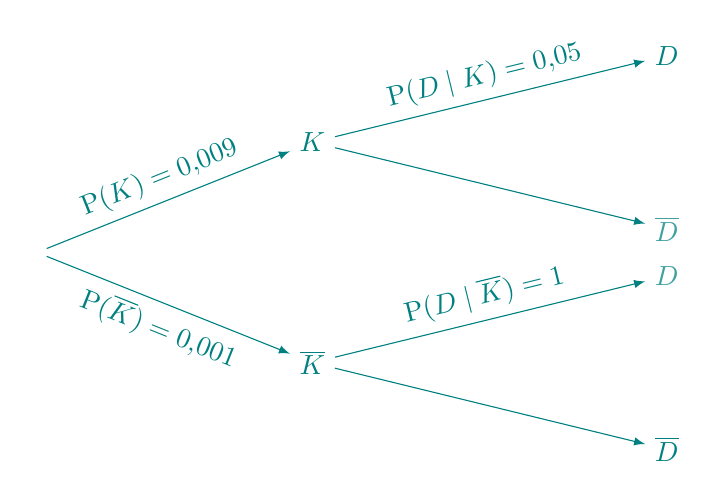
\begin{tikzpicture}[teal,grow=right, edge from parent/.style={draw,-latex}, label distance = 0.2cm,
					level 1/.style = {level distance=3.5cm, sibling distance=28mm},
					level 2/.style = {level distance=4.5cm, sibling distance=22mm},
					level 3/.style = {level distance=4.5cm, sibling distance=22mm},
					]
					
					\node {}
					child {node {$\overline{K}$ 
						}
						child {node {$\overline {D}$}
						}
						child {node[opacity=.75] {$D$}
							edge from parent
							node[above,sloped] {$\mathrm{P}(D\mid \overline {K})=1$}
						}
						edge from parent
						node[below,sloped] {$\mathrm{P}(\overline {K})=0{,}001$}
					}
					child {node[] {$K$} 
						child {node[opacity=.75] {$\overline {D}$}
						}
						child {node[] {$D$}	
							edge from parent
							node[above,sloped] {$\mathrm{P}(D\mid K)=0{,}05$}
						}
						edge from parent
						node[above,sloped] {$\mathrm{P}(K)=0{,}009$}
					};
				\end{tikzpicture}
			\end{center}
			\item Ta thấy, khả năng mắc bệnh của một người xét nghiệm có phản ứng dương tính chính là $\mathrm{P}(\overline{K} \mid D)$. Áp dụng công thức Bayes, ta có
			$$
			\mathrm{P}(\overline{K}|D)=\dfrac{\mathrm{P}(\overline{K}) \cdot \mathrm{P}(D| \overline{K})}{\mathrm{P}(\overline{K}) \cdot \mathrm{P}(D| \overline{K})+\mathrm{P}(K) \cdot \mathrm{P}(D| K)}=\dfrac{0{,}001}{0{,}001+0{,}999 \cdot 0{,}05} \approx 1{,}96 \% .
			$$			
			Vậy xác suất mắc bệnh của một người xét nghiệm có phản ứng dương tính là $1{,}96\%$.
		\end{itemize}		
	}
\end{bt}

\begin{bt}%[2D6C2-4]
% nguon: Archive/2024/TaiLieuGiangDay/6. K12 - 4in 1 - XsCoDieuKien/data/CHUONG 6 - XAC SUAT/OTC6-De-2.tex #3316
%[BAI-GIANG-12-4IN1, Võ Thị Thùy Trang]%[Cánh diều]
Giả sử trong một nhóm người có $2$ người nhiễm bệnh, $58$ người còn lại là không nhiễm bệnh. Để phát hiện ra người nhiễm bệnh, người ta tiến hành xét nghiệm tất cả mọi người của nhóm đó. Biết rằng đối với người nhiễm bệnh, xác suất xét nghiệm có kết quả dương tính là $85\%$, nhưng đối với người không nhiễm bệnh thì xác suất để bị xét nghiệm có phản ứng dương tính là $7\%$. Giả sử $X$ là một người trong nhóm bị xét nghiệm có kết quả dương tính. Tính xác suất để $X$ là người nhiễm bệnh (kết quả làm tròn đến hàng phần chục).
	\shortans{$0{,}3$}
	\loigiai{
		\begin{itemize}
			\item Xét hai biến cố\\
			$K$ \lq\lq Người được chọn không nhiễm bệnh\rq\rq.\\
			$D$ \lq\lq Người được chọn ra có kết quả dương tính\rq\rq.\\
			Nhóm người có $2$ người nhiễm bệnh, $58$ người còn lại là không nhiễm bệnh nên ta có $$\mathrm{P}(K)=\dfrac{58}{60}=\dfrac{29}{30};\, \mathrm{P}\left(\overline{K}\right)=\dfrac{2}{60}=\dfrac{1}{30}.$$
			Đối với người nhiễm bệnh, xác suất xét nghiệm có kết quả dương tính là $85\%$ nên\\ $\mathrm{P}\left(D|\overline{K}\right)=0{,}85$.\\
			Đối với người không nhiễm bệnh thì xác suất để bị xét nghiệm có phản ứng dương tính là $7\%$ nên $\mathrm{P}\left(D|K\right)=0{,}07$.\\
			Sơ đồ hình cây biểu thị tình huống trên
			\begin{center}
				\tikzstyle{level 1}=[level distance=3.5cm, sibling distance=3.5cm]
				\tikzstyle{level 2}=[level distance=3.5cm, sibling distance=2cm]
				\tikzstyle{pa} = [circle,inner sep=0pt]
				\tikzstyle{bag} = [text width=2em, text centered]
				\tikzstyle{end} = [minimum width=3pt,inner sep=4pt]
				\begin{tikzpicture}[grow=right, sloped,font=\footnotesize,>=stealth]
					\node[pa] {}
					child {
						node[bag] {$\overline{K}$}        
						child {
							node[end,right] {$\overline{D}$}
							edge from parent[->]
						}
						child {
							node[end,right] {$D$}
							edge from parent[->]
							node[above] {$\mathrm{P}\left(D|\overline{K}\right)=0{,}85$}
						}
						edge from parent[->]
						node[above] {$\mathrm{P}\left(\overline{K}\right)=\tfrac{1}{30}$}
					}
					child {
						node[bag] {$K$}        
						child {
							node[end,right] {$\overline{D}$}
							edge from parent[->]
						}
						child {
							node[end,right] {$D$}
							edge from parent[->]
							node[above] {$\mathrm{P}\left(D|K\right)=0{,}07$}
						}
						edge from parent[->]      
						node[above] {$\mathrm{P}(K)=\tfrac{29}{30}$}
					};
				\end{tikzpicture}
			\end{center}
			\item Áp dụng công thức xác suất toàn phần\\
			$\mathrm{P}(D)=\mathrm{P}(K)\cdot \mathrm{P}\left(D|K\right)+\mathrm{P}\left(\overline{K}\right)\cdot \mathrm{P}\left(D|\overline{K}\right)=\dfrac{29}{30}\cdot 0{,}07+\dfrac{1}{30}\cdot 0{,}85=0{,}096$.\\
			Áp dụng công thức xác suất Bayes\\
			$\mathrm{P}\left(\overline{K}|D\right)=\dfrac{\mathrm{P}\left(\overline{K}\right)\cdot \mathrm{P}\left(D|\overline{K}\right)}{\mathrm{P}(D)}=\dfrac{\dfrac{1}{30}\cdot 0{,}85}{0{,}096} \approx 0{,}3$.
		\end{itemize}
	}
\end{bt}

\begin{ex}%[2D6H2-2]
% nguon: Archive/SP_KhoLatex/SP_Đề Theo Bài-Khối 12/2-B19-De1.tex #3918

	Người ta khảo sát khả năng chơi nhạc cụ của một nhóm học sinh tại trường X. Nhóm này có $60\%$ học sinh là nam. Kết quả khảo sát cho thấy có $20\%$ học sinh nam và $15\%$ học sinh nữ biết chơi ít nhất một nhạc cụ. Chọn ngẫu nhiên một học sinh trong nhóm này. Gọi $A$ là biến cố \lq\lq Chọn được một học sinh biết chơi ít nhất một nhạc cụ\rq\rq\,và $B$, $\overline{B}$ lần lượt là các biến cố \lq\lq Chọn được một học sinh nam\rq\rq\,và \lq\lq Chọn được một học sinh nữ\rq\rq. 
	\choiceTF
	{\True Xác suất $\mathrm{P}(B) = 60\% = 0{,}6$}
	{$\mathrm{P}(A|B) = 0{,}8$}
	{\True $\mathrm{P}(A|\overline{B}) = 0{,}15$}
	{\True Xác suất để chọn được học sinh biết chơi ít nhất một nhạc cụ là $18\%$}
	\loigiai{
		Xét phép thử chọn ngẫu nhiên một học sinh trong nhóm.\\
		Gọi $A$ là biến cố \lq\lq Chọn được một học sinh biết chơi ít nhất một nhạc cụ\rq\rq \,và $B$, $\overline{B}$ lần lượt là các biến cố \lq\lq Chọn được một học sinh nam\rq\rq\,và \lq\lq Chọn được một học sinh nữ\rq\rq.
		Theo đề bài 
		\begin{itemchoice}
			\itemch $\mathrm{P}(B) = 60\% = 0{,}6$.
			$\mathrm{P}(\overline{B}) = 1-0{,}6 = 0{,}4$.
			\itemch $\mathrm{P}(A|B) = 20\% = 0{,}2$.
			\itemch $\mathrm{P}(A|\overline{B}) = 15\% = 0{,}15$. 
			\itemch Áp dụng công thức xác suất toàn phần, ta có
			$$\mathrm{P}(A) = \mathrm{P}(B)\cdot \mathrm{P}(A|B) + \mathrm{P}(\overline{B})\cdot \mathrm{P}(A|\overline{B}) = 0{,}6\cdot0{,}2 + 0{,}4\cdot 0{,}15 = 0{,}18.$$
			Vậy xác suất để chọn được một học sinh biết chơi nhạc cụ là $0{,}18$ hay $18\%$.
		\end{itemchoice}
	}
\end{ex}

\begin{ex}%[2D6H2-4]
% nguon: Archive/SP_KhoLatex/SP_Đề Theo Bài-Khối 12/2-B19-De1.tex #3919

	Kết quả khảo sát tại một xã cho thấy có $20\%$ cư dân hút thuốc lá. Tỉ lệ cư dân thường xuyên gặp các vấn đề sức khoẻ về đường hô hấp trong số những người hút thuốc lá và không hút thuốc lá lần lượt là $70\%$, $15\%$. Giả sử ta gặp một cư dân của xã, gọi $A$ là biến cố \lq\lq Người đó có hút thuốc lá\rq\rq\,và $B$ là biến cố \lq\lq Người đó thường xuyên gặp các vấn đề sức khoẻ về đường hô hấp\rq\rq.
	\choiceTF
	{$\mathrm{P}(AB)=0{,}13$}
	{$\mathrm{P}(\overline{A}B)=0{,}14$}
	{\True Nếu ta gặp một cư dân của xã thì xác suất người đó thường xuyên gặp các vấn đề sức khoẻ về đường hô hấp là $0{,}26$}
	{\True Nếu ta gặp một cư dân của xã thường xuyên gặp các vấn đề sức khoẻ về đường hô hấp thì xác suất người đó có hút thuốc lá xấp xỉ $54\%$}
	\loigiai{
		Giả sử ta gặp một cư dân của xã, gọi $A$ là biến cố \lq\lq Người đó có hút thuốc lá\rq\rq\,và $B$ là biến cố \lq\lq Người đó thường xuyên gặp các vấn đề sức khoẻ về đường hô hấp\rq\rq.\\
		Khi đó, ta có $\mathrm{P}(A)=0{,}2$; $\mathrm{P}(\overline{A})=0{,}8$; $\mathrm{P}(B|A)=0{,}7$, $\mathrm{P}(B|\overline{A})=0{,}15$.
		\begin{itemchoice}
			\itemch $\mathrm{P}(AB)=\mathrm{P}(A)\cdot \mathrm{P}(B|A)=0{,}2\cdot 0{,}7=0{,}14$.
			\itemch $\mathrm{P}(\overline{A}B)=\mathrm{P}(\overline{A})\cdot \mathrm{P}(B|\overline{A})=0{,}15\cdot0{,}8=0{,}12$.
			\itemch	
			Ta có $\mathrm{P}(B) = \mathrm{P}(A)\cdot \mathrm{P}(B|A) + \mathrm{P}(\overline{A})\cdot \mathrm{P}(B|\overline{A}) = 0{,}14 + 0{,}12 = 0{,}26$.\\
			Vậy nếu ta gặp một cư dân của xã thì xác suất người đó thường xuyên gặp các vấn đề sức khoẻ về đường hô hấp là $26\%$.
			\itemch Theo công thức Bayes, ta có $\mathrm{P}(A|B) = \dfrac{\mathrm{P}(A)\mathrm{P}(B|A)}{\mathrm{P}(B)} =\dfrac{ 0{,}2\cdot 0{,}7}{0{,} 26}\approx 0{,}54$.\\
			Vậy nếu ta gặp một cư dân của xã thường xuyên gặp các vấn đề sức khoẻ về đường hô hấp thì xác suất người đó có hút thuốc lá là khoảng $54\%$.
		\end{itemchoice}
	}
\end{ex}

\begin{ex}%[2D6H2-4]
% nguon: Archive/SP_KhoLatex/SP_Đề Theo Bài-Khối 12/2-B19-De1.tex #3920

	Xác suất để một chuyến bay khởi hành đúng giờ là $\mathrm{P}(D)=0{,}83$; xác suất để nó đến đúng giờ là $\mathrm{P}(A)=0{,}82$; xác suất để nó khởi hành và đến đều đúng giờ là $\mathrm{P}(D \cap A)=0{,}78$. 
	\choiceTF
	{\True Xác suất để một máy bay đến đúng giờ biết rằng nó đã khởi hành đúng giờ là $0{,}94$}
	{Xác suất để một máy bay khởi hành đúng giờ biết rằng nó sẽ đến đúng giờ là $0{,}85$}
	{\True Xác suất để một máy bay đến đúng giờ biết rằng nó khởi hành không đúng giờ là $0{,}24$}
	{Xác suất để một máy bay khởi hành đúng giờ biết rằng nó sẽ đến không đúng giờ là $0{,}95$}
	\loigiai{
		Ta có $\mathrm{P}(A \cap \overline{D})=\mathrm{P}(A)-\mathrm{P}(A \cap D)=0{,}82-0{,}78=0{,}04$.\\
		$\mathrm{P}(D \cap \overline{A})=\mathrm{P}(D)-\mathrm{P}(D \cap A)=0{,}83-0{,}78=0{,}05$.
		\begin{itemchoice}
			\itemch Xác suất để một máy bay đến đúng giờ biết rằng nó đã khởi hành đúng giờ là
			$$
			\mathrm{P}(A \mid D)=\frac{\mathrm{P}(D \cap A)}{\mathrm{P}(D)}=\frac{0{,}78}{0{,}83}=0{,}94.
			$$
			\itemch Xác suất để một máy bay khởi hành đúng giờ biết rằng nó đã đến đúng giờ là
			$$
			\mathrm{P}(D \mid A)=\frac{\mathrm{P}(D \cap A)}{\mathrm{P}(A)}=\frac{0{,}78}{0{,}82}=0{,}95.
			$$
			\itemch Xác suất để máy bay đến đúng giờ khi nó khởi hành không đúng giờ là
			$$
			\mathrm{P}(A \mid \overline{D})=\dfrac{\mathrm{P}(A \cap \overline{D})}{\mathrm{P}(\overline{D})}=\dfrac{0{,}82-0{,}78}{0{,}17}=0{,}24.
			$$
			\itemch Xác suất để một máy bay khởi hành đúng giờ biết rằng nó sẽ đến đúng giờ là $$
			\mathrm{P}(D \mid \overline{A})=\dfrac{\mathrm{P}(D \cap \overline{A})}{\mathrm{P}(\overline{A})}=\frac{0{,}83-0{,}78}{1-0{,}82}=0{,}28.
			$$
		\end{itemchoice}
	}
\end{ex}

\begin{bt}%[2D6V2-3]
% nguon: Archive/SP_KhoLatex/SP_Đề Theo Bài-Khối 12/2-B19-De1.tex #3922
%Câu 1
Có $7$ hộp bi, trong đó có $4$ hộp loại $1$, $3$ hộp loại $2$. Mỗi hộp loại $1$ có $3$ bi trắng và $5$ bi đỏ, mỗi hộp loại $2$ có $4$ bi trắng và $6$ bi đỏ. Chọn ngẫu nhiên $1$ hộp và từ đó lấy ra $1$ bi thì được bi trắng. Tìm xác suất để bi lấy ra này thuộc hộp loại $2$.  (Làm tròn đến kết quả hàng phần trăm).
	\shortans{$0{,}44$}
	\loigiai{ 
		Gọi $B$ là biến cố  \lq\lq lấy được bi trắng\rq\rq.\\
		$A_1$ là biến có lấy hộp loại 1.\\
		$A_2$ là biến có lấy hộp loại 2.\\
		$\mathrm{P}(A_1)=\dfrac{ \mathrm{C} _{4}^{1}}{ \mathrm{C} _{7}^{1}}=\dfrac{4}{7}$;
		$\mathrm{P}(A_2)=\dfrac{ \mathrm{C} _{3}^{1}}{ \mathrm{C} _{7}^{1}}=\dfrac{3}{7}$;
		$\mathrm{P}(B|A_1)=\dfrac{ \mathrm{C} _{3}^{1}}{ \mathrm{C} _{8}^{1}}=\dfrac{3}{8}$;
		$\mathrm{P}(B|A_2)=\dfrac{ \mathrm{C} _{4}^{1}}{ \mathrm{C} _{10}^{1}}=\dfrac{4}{10}=\dfrac{2}{5}$.\\
		$\Rightarrow \mathrm{P}(B)=\mathrm{P}(A_1)\mathrm{P}(B|A_1)+\mathrm{P}(A_2)\mathrm{P}(B|A_2)=\dfrac{4}{7}\cdot\dfrac{3}{8}+\dfrac{3}{7}\cdot\dfrac{2}{5}=\dfrac{27}{70}$.\\
		Xác suất để bi lấy ra này thuộc hộp loại $2$ là\\
		$\mathrm{P}(A_2|B)=\dfrac{\mathrm{P}(A_2)\mathrm{P}(B|A_2)}{\mathrm{P}(B)}=\dfrac{\dfrac{3}{7}\cdot\dfrac{2}{5}}{\dfrac{27}{70}}=\dfrac{4}{9}\approx 0{,}44$.
	}
\end{bt}

\begin{bt}%[2D6V2-2]
% nguon: Archive/SP_KhoLatex/SP_Đề Theo Bài-Khối 12/2-B19-De1.tex #3923
Câu 2
Trong $12$ xạ thủ có $5$ người bắn trúng hồng tâm với xác suất $0{,}8$; $7$ người bắn trúng hồng tâm với xác suất $0{,}7$. Chọn ngẫu nhiên $1$ xạ thủ. Tìm xác suất để người này bắn trúng hồng tâm.  (Làm tròn đến kết quả hàng phần trăm).
	\shortans{$0{,}74$}
	\loigiai{ Gọi $A$ là biến cố \lq\lq Xạ thủ bắn trúng hồng tâm\rq\rq.\\
	$A_1$ là biến cố \lq\lq nhóm $5$ người bắn trúng hồng tâm\rq\rq.\\
	$A_2$ là biến cố \lq\lq nhóm $7$ người bắn trúng hồng tâm\rq\rq.\\
	$\mathrm{P}(A_1)=\dfrac{5}{12}$; $\mathrm{P}(A_2)=\dfrac{7}{12}$;
	$\mathrm{P}(A|A_1)=0{,}8$; $P(A|A_2)=0{,}7$.\\
	Xác suất để người này bắn trúng hồng tâm
	$$\mathrm{P}(A)=\mathrm{P}(A_1)\mathrm{P}(A|A_1)+\mathrm{P}(A_1)P(A|A_2)=\dfrac{5}{12}\cdot0{,}8+\dfrac{7}{12}\cdot0{,}7=\dfrac{89}{120}\approx 0{,}74.$$
		}
\end{bt}

\begin{bt}%[2D6V2-2]
% nguon: Archive/SP_KhoLatex/SP_Đề Theo Bài-Khối 12/2-B19-De1.tex #3924
Câu 3
 Có $3$ hộp phấn. Hộp thứ nhất có $7$ viên trắng và $3$ viên vàng; hộp thứ hai có $16$ viên trắng và $4$ viên vàng; hộp thứ $3$ có $22$ viên trắng và $8$ viên vàng. Ta tung đồng thời $3$ đồng xu cân đối và đồng chất: nếu được cả $3$ mặt sấp thì chọn hộp thứ nhất; nếu được $1$ mặt sấp và $2$ mặt ngửa thì chọn hộp thứ hai; trường hợp còn lại thì chọn hộp thứ ba. Từ hộp đã chọn ta lấy ngẫu nhiên ra $1$ viên phấn. Tính xác suất để lấy được viên phấn trắng. (Làm tròn đến kết quả hàng phần trăm).
	\shortans{$0{,}75$}
	\loigiai{ 
		Gọi $A$ là biến cố \lq\lq Lấy được một viên phấn trắng\rq\rq.\\
		 $A_1$ là biến cố  \lq\lq Chọn hộp 1\rq\rq.\\
		 $A_2$ là biến cố \lq\lq Chọn hộp 2\rq\rq.\\
		 $A_3$ là biến cố \lq\lq Chọn hộp 3\rq\rq.\\
		 $\mathrm{P}(A_1)=\left ( \dfrac{1}{2} \right )^3$.\\ 
		 $\mathrm{P}(A_2)=3\cdot\dfrac{1}{2}\left ( \dfrac{1}{2} \right )^2=\dfrac{3}{8}$.\\ 
         $\mathrm{P}(A_3)=1-\dfrac{3}{8}-\dfrac{1}{8}=\dfrac{1}{2}$.\\	 
	 	  	$\mathrm{P}(A|A_1)=\dfrac{7}{10}$; $\mathrm{P}(A|A_2)=\dfrac{16}{20}=\dfrac{4}{5}$;$\mathrm{P}(A|A_3)=\dfrac{22}{30}=\dfrac{11}{15}$.\\
	 	  	Xác suất để lấy được viên phấn trắng
	 	   	\begin{eqnarray*}
	 	  	P(A)	& =& \mathrm{P}(A_1)\mathrm{P}(A|A_1)+\mathrm{P}(A_2)\mathrm{P}(A|A_2)+\mathrm{P}(A_3)\mathrm{P}(A|A_3)\\
	 	  		&= & \dfrac{1}{8}\cdot\dfrac{7}{10}+\dfrac{3}{8}\cdot\dfrac{4}{5}+\dfrac{1}{2}\cdot\dfrac{11}{5}\\
	 	  		& =& \dfrac{181}{240}\\
	 	  		&\approx &0{,75}.
	 	  	\end{eqnarray*}
	}
\end{bt}

\begin{bt}%[2D6C2-2]
% nguon: Archive/SP_KhoLatex/SP_Đề Theo Bài-Khối 12/2-B19-De1.tex #3925
%Câu 4
Một loại linh kiện do $3$ nhà máy số $I$, số $II$, số $III$ cùng sản xuất. Tỷ lệ phế phẩm của các nhà máy lần lượt là $I\colon 0{,}04$; $II\colon 0{,}03$ và $III\colon 0{,}05$. Trong $1$ lô linh kiện để lẫn lộn $80$ sản phẩm của nhà máy số $I$, $120$ của nhà máy số $II$ và $100$ của nhà máy số $III$. Một khách hàng lấy ngẫu nhiên 1 linh kiện từ lô hàng đó. Tính Xác suất để được linh kiện tốt?  (Làm tròn đến kết quả hàng phần trăm).
	\shortans{$0{,}96$}
	\loigiai{
		Gọi $E_1$ là biến cố \lq\lq phế phẩm máy số $I$\rq\rq $\Rightarrow \mathrm{P}(E_1)=0{,}04$; $\mathrm{P}(\overline{E_1})=0{,}96$.\\
		Gọi $E_2$ là biến cố \lq\lq phế phẩm máy số $II$\rq\rq $\Rightarrow \mathrm{P}(E_2)=0{,}03$; $\mathrm{P}(\overline{E_2})=0{,}97$.\\
		Gọi $E_3$ là biến cố \lq\lq phế phẩm máy số $III$\rq\rq $\Rightarrow P(E_1)=0{,}05$; $P(\overline{E_3})=0{,}95$.\\
		Gọi $B$ là biến cố khách hàng lấy được $1$ linh kiện tốt\\
		$\mathrm{P}(B|\overline{E_1})=\dfrac{\mathrm{C}_{80}^{1}}{\mathrm{C}_{300}^{1}}=\dfrac{4}{15}$;
		$\mathrm{P}(B|\overline{E_2})=\dfrac{\mathrm{C}_{120}^{1}}{\mathrm{C}_{300}^{1}}=\dfrac{2}{5}$;
		$\mathrm{P}(B|\overline{E_3})=\dfrac{\mathrm{C}_{100}^{1}}{\mathrm{C}_{300}^{1}}=\dfrac{1}{3}$.\\
		 Xác suất để khách hàng lấy được linh kiện tốt là
	\begin{eqnarray*}
			 	\mathrm{P}(B)	& =& \mathrm{P}(\overline{E_1})\mathrm{P}(B|\overline{E_1})+\mathrm{P}(E_2)\mathrm{P}(B|\overline{E_2})+\mathrm{P}(E_3)P(B|\overline{E_3})\\
		 	&= & 0{,}96\cdot\dfrac{4}{15}+0{,}97\cdot\dfrac{2}{5}+0{,}95\cdot\dfrac{1}{3}\\
		 	& =& \dfrac{181}{240}\\
		 	&\approx &0{,}96.
		 \end{eqnarray*}

	}
\end{bt}

\begin{bt}%[2D6C2-3]
% nguon: Archive/SP_KhoLatex/SP_Đề Theo Bài-Khối 12/2-B19-De1.tex #3926
Câu 5
Một loại linh kiện do $3$ nhà máy số $I$, số $II$, số $III$ cùng sản xuất. Tỷ lệ phế phẩm của các nhà máy lần lượt là: $I$: $0{,}04$; $II$: $0{,}03$ và $III$: $0{,}05$. Trong $1$ lô linh kiện để lẫn lộn $80$ sản phẩm của nhà máy số $I$, $120$ của nhà máy số $II$ và $100$ của nhà máy số $III$. Khách hàng lấy phải một linh kiện loại phế phẩm từ lô hàng đó. Khả năng linh kiện đó do nhà máy nào sản xuất là cao nhất?  (Làm tròn đến kết quả hàng phần trăm).
\shortans{$3$}
\loigiai{
	Gọi $E_1$ là biến cố \lq\lq phế phẩm máy số $I$\rq\rq $\Rightarrow \mathrm{P}(E_1)=0{,}04,\mathrm{P}(\overline{E_1})=0{,}96$.\\
	Gọi $E_2$ là biến cố \lq\lq phế phẩm máy số $II$\rq\rq $\Rightarrow \mathrm{P}(E_2)=0{,}03,\mathrm{P}(\overline{E_2})=0{,}97$.\\
	Gọi $E_3$ là biến cố \lq\lq phế phẩm máy số $III$\rq\rq $\Rightarrow \mathrm{P}(E_1)=0{,}05,\mathrm{P}(\overline{E_3})=0{,}95$\\
	Gọi $B$ là biến cố khách hàng lấy được $1$ linh kiện tốt\\
	$\mathrm{P}(B|\overline{E_1})=\dfrac{\mathrm{C}_{80}^{1}}{\mathrm{C}_{300}^{1}}=\dfrac{4}{15}$;
	$\mathrm{P}(B|\overline{E_2})=\dfrac{\mathrm{C}_{120}^{1}}{\mathrm{C}_{300}^{1}}=\dfrac{2}{5}$;
	$\mathrm{P}(B|\overline{E_3})=\dfrac{\mathrm{C}_{100}^{1}}{\mathrm{C}_{300}^{1}}=\dfrac{1}{3}$.\\
	Xác suất để khách hàng lấy được linh kiện tốt là\allowdisplaybreaks
	\begin{eqnarray*}
	\mathrm{P}(B)&=&\mathrm{P}(\overline{E_1})\mathrm{P}(B|\overline{E_1})+P(\overline{E_2})\mathrm{P}(B|\overline{E_2})+\mathrm{P}(\overline{E_3})\mathrm{P}(B|\overline{E_3})\\
	&=&0{,}96\cdot\dfrac{4}{15}+0{,}97\cdot\dfrac{2}{5}+0{,}95\cdot\dfrac{1}{3}\approx 0{,}96.
	\end{eqnarray*}
	Gọi $\overline{B}$ là biến cố khách hàng lấy $1$ linh kiện loại không tốt\\
			 $\mathrm{P}(\overline{B})=1-\mathrm{P}(B)=0{,}04$.\\
	$\mathrm{P}(E_1|\overline{B})=\dfrac{\mathrm{P}(E_1)P(\overline{B}|E_1)}{\mathrm{P}(\overline{B})}=\dfrac{0{,}04 \cdot \dfrac{\mathrm{C}_{80}^{1}}{\mathrm{C}_{300}^{1}}}{0{,}04}=0{,}26$.\\
	$\mathrm{P}(E_2|\overline{B})=\dfrac{\mathrm{P}(E_2)\mathrm{P}(\overline{B}|E_2)}{\mathrm{P}(\overline{B})}=\dfrac{0{,}03 \cdot \dfrac{\mathrm{C}_{120}^{1}}{\mathrm{C}_{300}^{1}}}{0{,}04}=0{,}3$.\\
	$\mathrm{P}(E_3|\overline{B})=\dfrac{\mathrm{P}(E_3)P(\overline{B}|E_3)}{\mathrm{P}(\overline{B})}=\dfrac{0{,}05 \cdot \dfrac{\mathrm{C}_{100}^{1}}{\mathrm{C}_{300}^{1}}}{0{,}04}=0{,}41$.\\
	Vậy linh kiện đó do máy $III$ là cao nhất.
	}
\end{bt}

\begin{bt}%[2D6V2-3]
% nguon: Archive/SP_KhoLatex/SP_Đề Theo Bài-Khối 12/2-B19-De1.tex #3927
Câu 6
	Trong $1$ đám đông, số người nam bằng số người nữ. Xác suất mắc cận thị của nam là $0{,}4$ và nữ là $0{,}6$. Chọn ngẫu nhiên $1$ người. Xác suất chọn được nam không cận thị. (Làm tròn đến kết quả hàng phần trăm).
	\shortans{$0{,}6$}
	\loigiai{ Goi tiêp $H_1$ là biến cố chọn nam; $H_2$ là biến cố chọn được nữ.\\
		$C$ là biến cố người được chọn là không cận thị.\\
		Ta có $\mathrm{P}(H_1)=\mathrm{P}(H_2)=\dfrac{1}{2}$\\
		 $\mathrm{P}(C)=\mathrm{P}(H_1)\mathrm{P}(C|H_1)+\mathrm{P}(H_2)\mathrm{P}(C|H_2)=\dfrac{1}{2}\cdot0{,}6+\dfrac{1}{2}\cdot0{,}4=0{,}5$.\\
		Xác suất để chọn ngẫu nhiên ra $1$ người mà người đó là nam không cận thị là\\ (Áp dụng định lý Bayes)\\
		$\mathrm{P}(H_1|C)=\dfrac{\mathrm{P}(H_1)\mathrm{P}(C|H_1)}{\mathrm{P}(C)}=\dfrac{\dfrac{1}{2}\cdot0{,}6}{0{,}5}=0{,}6$.}
	\end{bt}

\begin{ex}%[2D6V1-2]
% nguon: Archive/SP_KhoLatex/SP_Đề Theo Bài-Khối 12/2-OTC6-De2.tex #3948
%[Nguyễn Khánh Trọng]
	Một nhà máy thực hiện khảo sát toàn bộ công nhân về sự hài lòng của họ về điều kiện làm việc tại phân xưởng. Kết quả khảo sát như sau:
	\begin{center}
		\begin{tabular}{|c|ccll|}
			\hline
			\multirow{2}{*}{Khảo sát công nhân} & \multicolumn{4}{c|}{Kết quả khảo sát}                               \\ \cline{2-5} 
			& \multicolumn{1}{c|}{Hài lòng} & \multicolumn{3}{c|}{Không hài lòng} \\ \hline
			Số công nhân xưởng I                & \multicolumn{1}{c|}{23}       & \multicolumn{3}{c|}{12}             \\ \hline
			Số công nhân xưởng II               & \multicolumn{1}{c|}{25}       & \multicolumn{3}{c|}{15}             \\ \hline
		\end{tabular}
	\end{center}
	Gặp ngẫu nhiên một công nhân của nhà máy. Gọi $A$ là biến cố \lq\lq Công nhân đó làm việc tại phân xưởng I\rq\rq \, và $B$ là biến cố \lq\lq Công nhân đó hài lòng với điều kiện làm việc tại phân xưởng\rq\rq. Xét tính đúng sai của các phát biểu sau.
	\choiceTF
	{\True Xác suất của biến cố $A$ là $\dfrac{7}{15}$}
	{Xác suất của biến cố $B$ là $0{,}65$}
	{\True Xác suất gặp được công nhân không hài lòng với điều kiện làm việc tại phân xưởng biết công nhân đó thuộc xưởng I là $\dfrac{12}{35}$}
	{Xác suất gặp được công nhân thuộc xưởng II biết công nhân đó hài lòng với điều kiện làm việc tại phân xưởng là $0{,}52$}
	\loigiai{
		Gặp ngẫu nhiên một công nhân của nhà máy, ta có $n(\Omega)=23+12+25+15=75$. 
		\begin{itemchoice}
			\itemch {\bf Đúng.}\\
			Ta có $n(A)=23+12=35$.\\
			Xác suất của biến cố $A$ là 
			$\mathrm{P}(A)=\dfrac{35}{75}=\dfrac{7}{15}$.
			\itemch  {\bf Sai.} \\
			Ta có $n(B)=23+25=48$. \\
			Xác suất của biến cố $B$ là 
			$\mathrm{P}(B)=\dfrac{48}{75}=\dfrac{16}{25}$.
			\itemch Đúng. Ta có $n(\overline{B}A)=12\Rightarrow \mathrm{P}(\overline{B}A)=\dfrac{12}{75}=\dfrac{4}{25}$.\\
			Do đó
			$\mathrm{P}(\overline{B}\mid A)=\dfrac{\mathrm{P}(\overline{B}A)}{\mathrm{P}(A)}=\dfrac{\dfrac{4}{25}}{\dfrac{7}{15}}=\dfrac{12}{35}$.
			\itemch {\bf Sai.}\\
			 Ta có $n(\overline{A}B)=25\Rightarrow\mathrm{P}(\overline{A}B)
			 =\dfrac{25}{75}=\dfrac{1}{3}$.\\
			Do đó
			$\mathrm{P}(\overline{A}\mid B)=\dfrac{\mathrm{P}(\overline{A}B)}{\mathrm{P}(B)}
			=\dfrac{\dfrac{1}{3}}{\dfrac{16}{25}}=\dfrac{25}{48}$.
		\end{itemchoice}
	}
\end{ex}

\begin{ex}%[2D6V2-2]
% nguon: Archive/SP_KhoLatex/SP_Đề Theo Bài-Khối 12/2-OTC6-De2.tex #3951
%[Nguyễn Khánh Trọng]
	Trong một trường học, tỉ lệ học sinh nữ là $55\%$. Tỉ lệ học sinh nữ và tỉ lệ học sinh nam tham gia câu lạc bộ tiếng anh lần lượt là $20\%$ và $15\%$. Gặp ngẫu nhiên $1$ học sinh của trường. 
	Gọi $A$ là biến cố \lq\lq Học sinh đó là nữ\rq\rq\, và $B$ là biến cố \lq\lq Học sinh đó tham gia câu lạc bộ tiếng Anh\rq\rq. Xét tính đúng sai của các phát biểu sau.
	\choiceTF
	{\True $\mathrm{P}(\overline{A})=0{,}45$}
	{$\mathrm{P}(B\mid \overline{A}) = 0{,}15$ và $\mathrm{P}(\overline{B}\mid A) = 0{,}2$}
	{Xác suất để học sinh đó có tham gia câu lạc bộ tiếng Anh là $0{,}1675$}
	{\True Biết rằng học sinh có tham gia câu lạc bộ tiếng Anh. Xác suất học sinh đó là nam bằng $\dfrac{27}{71}$}
	\loigiai{
			\begin{itemchoice}
			\itemch {\bf Đúng.}\\
			Do tỉ lệ học sinh nữ là $55\%$ nên
			$\mathrm{P}(A) = 0{,}55$ và $\mathrm{P}(\overline{A}) = 1 - 0{,}55 = 0{,}45$.
			\itemch {\bf Sai.}\\
			Do tỉ lệ học sinh nữ và tỉ lệ học sinh nam tham gia câu lạc bộ tiếng Anh lần lượt là $20\%$ và $15\%$ nên $\mathrm{P}(B\mid A) = 0{,}2$ và $\mathrm{P}(B\mid \overline{A}) = 0{,}15$.\\
			Suy ra $\mathrm{P}(\overline{B}\mid A) =1-\mathrm{P}(B\mid A)=1-0{,}2=0{,}8$.
			\itemch {\bf Sai.}\\
		Xác suất để học sinh đó có tham gia câu lạc bộ tiếng Anh là
		$$\mathrm{P}(B) = \mathrm{P}(A)\cdot\mathrm{P}(B\mid A) + \mathrm{P}(\overline{A})\cdot\mathrm{P}(B\mid\overline{A}) = 0{,}55 \cdot 0{,}2 + 0{,}45 \cdot 0{,}15 = 0{,}1775.$$
			\itemch {\bf Đúng.}\\
			Do học sinh có tham gia câu lạc bộ tiếng Anh nên xác suất học sinh đó là nam là
			$$\mathrm{P}(\overline{A}\mid B) = \dfrac{\mathrm{P}(\overline{A})\cdot \mathrm{P}(B\mid \overline{A})}{\mathrm{P}(B)}=
			\dfrac{0{,}45\cdot 0{,}15}{0{,}1775}=\dfrac{27}{71}.$$
		\end{itemchoice}
	}
\end{ex}

\begin{bt}%[2D6V1-2]
% nguon: Archive/SP_KhoLatex/SP_Đề Theo Bài-Khối 12/2-OTC6-De2.tex #3952
%[Võ Thanh Hiệp]
Lớp 12A có $40$ học sinh, trong đó có $22$ bạn nữ và $18$ bạn nam. Có $3$ tên Hiền gồm hai bạn nam  và một bạn nữ. Thầy giáo chọn ngẫu nhiên một bạn lên bảng làm bài tập. Tính xác suất để chọn đúng bạn tên Hiền là bạn nam  ({\it kết quả làm tròn đến hàng phần trăm}).

	\shortans{$0{,}25$}
	\loigiai{
Gọi $A$ là biến cố: \lq\lq Chọn bạn tên Hiền\rq\rq.\\
Gọi $B$ là biến cố: \lq\lq Chọn bạn nam\rq\rq.\\
Ta có $\mathrm{P}\left(A\right) = \dfrac{3}{40}$,
 $\mathrm{P}\left(B\right) = \dfrac{18}{40}=\dfrac{9}{20}$, 
 $\mathrm{P}\left(AB\right) = \dfrac{2}{18}=\dfrac{1}{9}$.\\
Xác suất chọn đúng bạn tên Hiền với điều kiện là bạn nam $\mathrm{P}\left(A\mid B\right)$.\\
Ta có $\mathrm{P}\left(A\mid B\right)=\dfrac{\mathrm{P}\left(AB\right)}{\mathrm{P}\left(B\right)}=
\dfrac{20}{81} \approx 0{,}25$.
	}
\end{bt}

\begin{bt}%[2D6V1-2]
% nguon: Archive/SP_KhoLatex/SP_Đề Theo Bài-Khối 12/2-OTC6-De2.tex #3953
%[Võ Thanh Hiệp]
Một hộp đựng $30$ viên bi kích thước, chất liệu như nhau, trong đó có $20$ viên bi xanh và $10$ viên bi trắng. Lấy ngẫu nhiên ra một viên bi không bỏ lại trong hộp, rồi lại lấy ngẫu nhiên ra một viên bi nữa. Tính xác suất để lấy được một viên bi trắng  ở lần thứ nhất và một viên bi xanh ở lần thứ hai ({\it kết quả làm tròn đến hàng phần trăm}).
	\shortans{$0{,}23$}
	\loigiai{
Gọi $A$ là biến cố: \lq\lq Lấy được một viên bi trắng  ở lần thứ nhất\rq\rq.\\
Gọi $B$ là biến cố: \lq\lq Lấy được một viên bi xanh  ở lần thứ hai\rq\rq.\\
Ta có $P\left(A\right) = \dfrac{10}{30}=\dfrac{1}{3}$.\\
Nếu $A$ đã xảy ra, tức là một viên bi trắng đã được lấy ra ở lần thứ nhất, thì còn lại trong hộp $29$ viên bi trong đó số viên bi xanh là 20, do đó $P\left(B\mid A\right)=\dfrac{20}{29}$.\\
Xác suất để lấy được một viên bi trắng  ở lần thứ nhất và một viên bi xanh ở lần thứ hai là $P\left(A B\right)$.\\
Ta có $P\left(A B\right) = P\left(A\right) \cdot P\left(B\mid A\right)=
 \dfrac{1}{3} \cdot \dfrac{20}{29}=\dfrac{20}{87}\approx 0{,}23$.
	}
\end{bt}

\begin{bt}%[2D6V2-2]
% nguon: Archive/SP_KhoLatex/SP_Đề Theo Bài-Khối 12/2-OTC6-De2.tex #3954
%[Võ Thanh Hiệp]
Khảo sát tỉ lệ người dân trong một xã nghiện thuốc lá là $20\%$; tỉ lệ người bị bệnh phổi trong số người nghiện thuốc lá là $70\%$, trong số người không nghiện thuốc lá là $15\%$. Hỏi khi ta gặp ngẫu nhiên một người dân của của xã đó thì khả năng mà người đó bị bệnh phổi là bao nhiêu $\%$?
	\shortans{$26$}
	\loigiai{
Gọi $A$ là biến cố: \lq\lq Người nghiện thuốc lá\rq\rq.\\
Suy ra $\overline{A}$ là biến cố: \lq\lq Người không nghiện thuốc lá\rq\rq. \\
Gọi $B$ là biến cố: \lq\lq Người bị bệnh phổi\rq\rq.\\
Xác suất người nghiện thuốc lá là $\mathrm{P}\left(A\right) = 20\% = 0{,}2$.\\
Xác suất người không nghiện thuốc lá là  $\mathrm{P}\left(\overline{A}\right) =1- \mathrm{P}\left(A\right) = 0{,}8$.\\
Xác suất người bị bệnh phổi trong số người nghiện thuốc lá là $70\% \Rightarrow \mathrm{P}\left(B\mid A\right) = 0{,}7$.\\
Xác suất người bị bệnh phổi không nghiện thuốc lá là $15\% \Rightarrow \mathrm{P}\left(B\mid \overline{A}\right) = 0{,}15$.\\
Xác suất người bị bệnh phổi là\\
$\mathrm{P}\left(B\right) = \mathrm{P}\left(A\right) \cdot \mathrm{P}\left(B\mid A\right)+
\mathrm{P}\left(\overline{A}\right) \cdot \mathrm{P}\left(B\mid \overline{A}\right)
= 0{,}2\cdot 0{,}7+0{,}8\cdot 0{,}15=0{,}26=26\%$.
	}
\end{bt}

\begin{bt}%[2D6V2-3]
% nguon: Archive/SP_KhoLatex/SP_Đề Theo Bài-Khối 12/2-OTC6-De2.tex #3956
%[Võ Thanh Hiệp]
Khảo sát sự yêu thích môn Toán của hai lớp 12 của một trường. Lớp 12A1 có 40 học sinh và có $80\%$ học sinh thích môn Toán, lớp 12A2 có 32 học sinh và có $75\%$ học sinh thích môn Toán. Chọn ngẫu nhiên một học sinh. Biết rằng bạn đó yêu thích môn Toán, tính xác suất bạn đó học lớp 12A1 ({\it kết quả làm tròn đến hàng phần trăm}).
	\shortans{$0{,}57$}
	\loigiai{
Gọi $A$ là biến cố: \lq\lq Học sinh yêu thích môn Toán\rq\rq.\\
Gọi $B$ là biến cố: \lq\lq Học sinh lớp 12A1\rq\rq.\\
Gọi $C$ là biến cố: \lq\lq Học sinh lớp 12A2\rq\rq.\\	
Theo đề bài ta có\\
$\mathrm{P}\left(B\right) = \dfrac{40}{72} =\dfrac{5}{9}$;
$\mathrm{P}\left(C\right) = \dfrac{32}{72} =\dfrac{4}{9}$;
$\mathrm{P}\left(A\mid B\right) = 80\% =\dfrac{4}{5}$;
 $\mathrm{P}\left(A\mid C\right) = 75\% =\dfrac{3}{4}$.\\ 
Áp dụng công thức xác suất toàn phần, ta có\\
$\mathrm{P}\left(A\right) = \mathrm{P}\left(B\right) \cdot \mathrm{P}\left(A\mid B\right)+
\mathrm{P}\left(C\right) \cdot \mathrm{P}\left(A\mid C\right)
= \dfrac{5}{9}\cdot \dfrac{4}{5}+ \dfrac{4}{9}\cdot \dfrac{3}{4}=\dfrac{7}{9}$.\\
Xác suất cần tìm là 
$\mathrm{P}\left(B\mid A\right)=
\dfrac{\mathrm{P}\left(A\mid B\right)\cdot \mathrm{P}\left(B\right) }{\mathrm{P}\left(A\right)}=
\dfrac{\dfrac{4}{5}\cdot\dfrac{5}{9}}{\dfrac{7}{9}}=\dfrac{4}{7}\approx 0{,}57$.
	}
\end{bt}

\begin{bt}%[2D6V2-3]
% nguon: Archive/SP_KhoLatex/SP_Đề Theo Bài-Khối 12/2-OTC6-De2.tex #3957
%[Võ Thanh Hiệp]
Hộp thứ nhất có 6 viên bi đỏ và 4 viên bi xanh, hộp thứ hai có 4 viên bi đỏ và 6 viên bi xanh, các viên bi có cùng khối lượng và kích thước. Lấy ngẫu nhiên 1 viên bi từ hộp thứ nhất bỏ sang hộp thứ hai. Sau đó từ hộp thứ hai lấy ngẫu nhiên ra một viên bi. Biết rằng viên bi lấy ra từ hộp hai là viên bi màu đỏ. Tính xác suất viên bi bỏ từ hộp thứ nhất sang hộp thứ hai là màu xanh ({\it kết quả làm tròn đến hàng phần trăm}).
	
	\shortans{$0{,}35$}
	\loigiai{
Gọi $A$ là biến cố: \lq\lq Bi bỏ từ hộp thứ nhất sang hộp thứ hai là bi màu xanh \rq\rq.\\	
Suy ra  $\overline{A}$ là biến cố: \lq\lq Bi bỏ từ hộp thứ nhất sang hộp thứ hai là bi màu đỏ \rq\rq.\\
Gọi $B$ là biến cố: \lq\lq Bi lấy từ hộp thứ hai là bi màu đỏ \rq\rq.\\		
Theo đề bài ta có\\
$\mathrm{P}\left(A\right)= \dfrac{4}{10}$;
$\mathrm{P}\left(\overline{A}\right)= \dfrac{6}{10}$;
$\mathrm{P}\left(B\mid A\right)=\dfrac{4}{11}$;
$\mathrm{P}\left(B\mid \overline{A}\right)=\dfrac{5}{11}$.\\
Áp dụng công thức xác suất toàn phần, ta có\\
$\mathrm{P}\left(B\right) =\mathrm{P}\left(A\right) \cdot \mathrm{P}\left(B\mid A\right)+
\mathrm{P}\left(\overline{A}\right) \cdot \mathrm{P}\left(B\mid \overline{A}\right)=
\dfrac{4}{10}\cdot\dfrac{4}{11}+ \dfrac{6}{10}\cdot\dfrac{5}{11}=\dfrac{23}{55}$.\\
Xác suất cần tìm là 
$\mathrm{P}\left(A\mid B\right)=
\dfrac{\mathrm{P}\left(B\mid A\right)\cdot \mathrm{P}\left(A\right) }{\mathrm{P}\left(B\right)}=
\dfrac{\dfrac{4}{11}\cdot\dfrac{4}{10}}{\dfrac{23}{55}}=\dfrac{8}{23}\approx 0{,}35$.
	}
\end{bt}

\begin{bt}%[2D6V2-2]
% nguon: Archive/SP_KhoLatex/SP_Đề Theo Bài-Khối 12/2-OTCK2-De1.tex #3962

	Một nghiên cứu đã chỉ ra rằng tỉ lệ người bị lao phổi trong nhóm $X$ những người mắc phải hội chứng suy giảm miễn dịch $H$ là $15{,}2 \%$. Kết quả nghiên cứu về một số triệu chứng lâm sàng như có ho trong vòng bốn tuần, hoặc có bị sốt trong vòng bốn tuần, hoặc ra mồ hôi ban đêm từ ba tuần trở lên của nhóm $X$ cho thấy.
	\begin{itemize}
		\item Trong số những người mắc bệnh lao phổi, có $93{,}2 \%$ trường hợp có ít nhất một triệu chứng;
		\item Trong số những người không mắc bệnh lao phổi, có $35{,}8 \%$ trường hợp không có triệu chứng nào.
	\end{itemize}
	Nếu bác sĩ gặp một bệnh nhân thuộc nhóm $X$ và bệnh nhân đó có ít nhất một triệu chứng trên thì xác suất bệnh nhân này mắc bệnh lao phổi là bao nhiêu? (kết quả làm tròn đến phần trăm)
	\shortans[]{$0,21$}
	\loigiai{
		Gọi $A$ là biến cố \lq\lq Người bị lao phổi\rq\rq.\\
		$\overline{A}$ là biến cố \lq\lq Người không mắc lao phổi\rq\rq.\\
		$B$ là biến cố \lq\lq Những người có ít nhất một triệu chứng\rq\rq.\\
		$\overline{B}$ là biến cố \lq\lq Những người không có triệu chứng\rq\rq.\\
		Ta có $\mathrm{P}(A)=0{,}152$. \\
		Khi đó, xác suất những người không mắc lao phổi là $$\mathrm{P}\left(\overline{A}\right)=1-0{,}152=0{,}848.$$
		Ta có xác suất những người có ít một triệu chứng trong những người mắc lao phổi là $$\mathrm{P}\left(B|A\right)=0{,}932.$$
		Khi đó, xác suất những người không có triệu chứng trong những người mắc lao phổi là  $$\mathrm{P}\left(\overline{B}|A\right)=1-0{,}932=0{,}068.$$
		Mặt khác, ta có xác suất những người không có triệu chứng  $$\mathrm{P}\left(\overline{B}|\overline{A}\right)=0{,}358.$$
		Khi đó, xác suất những người có ít nhất một triệu chứng trong những người không mắc bệnh lao phổi là $$\mathrm{P}\left(B|\overline{A}\right)=1-0{,}358=0{,}642.$$
		Ta có $\mathrm{P}(B)=\mathrm{P}\left(B|A\right)\cdot \mathrm{P}(A)+\mathrm{P}\left(B|\overline{A}\right)\cdot \mathrm{P}\left(\overline{A}\right)=0{,}932\cdot 0{,}152+0{,}642\cdot 0{,}848=0{,}68608$.\\
		Theo công thức Bayes, ta có $\mathrm{P}(A|B)=\dfrac{\mathrm{P}(A)\cdot\mathrm{P}\left(B|A\right)}{\mathrm{P}(B)}=\dfrac{0{,}152\cdot 0{,}932}{0{,}68608}\approx 0{,}2065$.
	}
\end{bt}

\begin{bt}%[2D6V2-3]
% nguon: Archive/SP_KhoLatex/SP_Đề Theo Bài-Khối 12/2-OTCK2-De1.tex #3963

	Bạn Nam tham gia một gian hàng trò chơi dân gian trong hội xuân của trường. Trò chơi có hai lượt chơi. Xác suất để Nam thắng ở lượt chơi thứ nhất là $0{,}6$. Nếu Nam thắng ở lượt chơi thứ nhất thì xác suất Nam thắng ở lượt chơi thứ hai là $0{,}8$. Ngược lại, nếu Nam thua ở lượt chơi thứ nhất thì xác suất Nam thắng ở lượt chơi thứ hai là $0{,}3$. Biết Nam đã thắng ở lượt chơi thứ hai, tính xác suất Nam thắng ở lượt chơi thứ nhất.
	\shortans[]{$0,8$}
	\loigiai{
		Công thức Bayes cho sự kiện $A$ và $B$ là $\mathrm{P}(A | B)=\dfrac{\mathrm{P}(B | A) \cdot \mathrm{P}(A)}{\mathrm{P}(B)}$.\\
		Trong đó
		\begin{itemize}
			\item $A$ là biến cố \lq\lq Nam thắng ở lượt chơi thứ nhất\rq\rq.
			\item $B$ là biến cố \lq\lq Nam thắng ở lượt chơi thứ hai\rq\rq.
			\item $\mathrm{P}(A)$ là xác suất Nam thắng ở lượt chơi thứ nhất $\Rightarrow \mathrm{P}(A) = 0{,}6$.
			\item $\mathrm{P}(B | A)$ là xác suất Nam thắng ở lượt chơi thứ hai khi đã thắng ở lượt chơi thứ nhất $\Rightarrow \mathrm{P}(B | A) = 0{,}8$.
			\item $\mathrm{P}(B | \overline{A})$ là xác suất Nam thắng ở lượt chơi thứ hai khi đã thua ở lượt chơi thứ nhất $\Rightarrow \mathrm{P}(B | \overline{A} = 0{,}3$.
		\end{itemize}
		Công thức Bayes
		$$
		\begin{aligned}[t]
			\mathrm{P}(A | B)&=\dfrac{\mathrm{P}(B | A) \cdot \mathrm{P}(A)}{\mathrm{P}(B | A) \cdot \mathrm{P}(A)+\mathrm{P}(B | \overline{A}) \cdot \mathrm{P}(\overline{A})} \\
			& =\dfrac{(0{,}8) \cdot(0.6)}{(0{,}8) \cdot(0{,}6)+(0{,}3) \cdot(0{,}4)} \\
			& \approx \dfrac{0{,}48}{0{,}48+0{,}12} \\
			& \approx \dfrac{0.48}{0.6} \\
			& \approx 0{,}8.
		\end{aligned}
		$$
		Vậy, xác suất Nam thắng ở lượt chơi thứ nhất khi đã thắng ở lượt chơi thứ hai là khoảng $0{,}8$ hoặc $80 \%$.
	}
\end{bt}

\begin{ex}%[2D6V1-3]
% nguon: Archive/SP_KhoLatex/SP_Đề Theo Bài-Khối 12/2-OTC6-De1.tex #3986

	Trong một hộp có $18$ quả bóng bàn loại I và $2$ quả bóng bàn loại II, các quả bóng bàn có hình dạng và kích thước như nhau. Một học sinh lấy ngẫu nhiên lần lượt $2$ quả bóng bàn (lấy không hoàn lại) trong hộp.\\ Xét tính đúng, sai của các khẳng định sau
	\choiceTF
	{Xác suất để lần thứ nhất lấy được quả bóng bàn loại II là $\dfrac{9}{10}$}
	{\True Xác suất để lần thứ hai lấy được quả bóng bàn loại II, biết lần thứ nhất lấy được quả bóng bàn loại II, là $\dfrac{1}{19}$}
	{Xác suất để cả hai lần đều lấy được quả bóng bàn loại II là $\dfrac{9}{190}$}
	{\True Xác suất để ít nhất $1$ lần lấy được quả bóng bàn loại I là $\dfrac{189}{190}$}
	\loigiai{
	Xét các biến cố\\
	$A\colon$ \lq\lq Lần thứ nhất lấy được quả bóng bàn loại II\rq\rq;\\
	$B\colon$ \lq\lq Lần thứ hai lấy được quả bóng bàn loại II\rq\rq. 
	\begin{itemchoice}
	\itemch Sai, vì Xác suất để lần thứ nhất lấy được quả bóng bàn loại II là $\mathrm{P}(A)=\dfrac{2}{20}=\dfrac{1}{10}$.
	\itemch Đúng, vì sau khi lấy $1$ quả bóng bàn loại II thì chỉ còn $1$ quả bóng bàn loại II trong hộp.\\ Suy ra xác suất để lần thứ hai lấy được quả bóng bàn loại II, biết lần thứ nhất lấy được quả bóng bàn loại II là $\mathrm{P}(B | A)=\dfrac{1}{19}$.
	\itemch Sai, vì xác suất để cả hai lần đều lấy được quả bóng bàn loại II là
	$$
	\mathrm{P}(C)=\mathrm{P}(A \cap B)=\mathrm{P}(A) \cdot \mathrm{P}(B | A)=\dfrac{1}{10} \cdot \dfrac{1}{19}=\dfrac{1}{190}.
	$$
	\itemch Đúng, vì để ít nhất $1$ lần lấy được quả bóng bàn loại I là
	$$
	\mathrm{P}(\overline {C})=1-\mathrm{P}(C)=1-\frac{1}{190}=\frac{189}{190} \text {. }
	$$
	\end{itemchoice}
	}
\end{ex}

\begin{bt}%[2D6V2-2]
% nguon: Archive/SP_KhoLatex/SP_Đề Theo Bài-Khối 12/2-OTC6-De1.tex #3988

	Có hai hộp đựng các viên bi cùng kích thước và khối lượng. Hộp thứ nhất chứa $5$ viên bi đỏ và $5$ viên bi xanh, hộp thứ hai chứa $6$ viên bi đỏ và $4$ viên bi xanh. Lấy ngẫu nhiên một viên bi từ hộp thứ nhất chuyển sang hộp thứ hai, sau đó lấy ra ngẫu nhiên một viên bi từ hộp thứ hai. Tính xác suất để viên bi được lấy ra từ hộp thứ hai là viên bi đỏ (làm tròn đến hàng phần trăm).
	\shortans{$0{,}59$}
	\loigiai{
	Xét phép thử lấy ngẫu nhiên một viên bi từ hộp thứ nhất chuyển sang hộp thứ hai, sau đó lấy ra ngẫu nhiên một viên bi từ hộp thứ hai. Xét các biến cố sau
	\begin{itemize}
	\item $A$ là biến cố \lq \lq Viên bi được lấy ra từ hộp thứ hai là bi đỏ \rq \rq;
	\item $C$ là biến cố \lq \lq Viên bi được lấy ra từ hộp thứ hai là bi của hộp thứ nhất \rq \rq;
	\item $\overline{C}$ là biến cố \lq \lq Viên bi được lấy ra từ hộp thứ hai là bi của hộp thứ hai\rq \rq.
	\end{itemize}
	Sau khi chuyển một viên bi từ hộp thứ nhất sang hộp thứ hai thì hộp thứ hai có $11$ viên bi. Ta có 
	$$\mathrm{P}(C)=\dfrac{1}{11};\, \mathrm{P}(\overline{C})=\dfrac{10}{11}.$$
	Xác suất để viên bi được lấy ra từ hộp thứ hai là bi đỏ của hộp thứ nhất 
	$$\mathrm{P}(A\mid C)=\dfrac{5}{10}=\dfrac{1}{2}.$$
	Xác suất để viên bi được lấy ra từ hộp thứ hai là bi đỏ của hộp thứ hai 
	$$\mathrm{P}(A\mid \overline{C})=\dfrac{6}{10}=\dfrac{3}{5}.$$
	Áp dụng công thức xác suất toàn phần, ta có
	$$\mathrm{P}(A) = \mathrm{P}(C)\cdot \mathrm{P}(A\mid C) + \mathrm{P}(\overline{C})\cdot P(A\mid \overline{C}) =\dfrac{1}{11}\cdot \dfrac{1}{2}+\dfrac{10}{11}\cdot \dfrac{3}{5}=\dfrac{13}{22}\approx 0{,}59.$$
	}
\end{bt}

\begin{bt}%[2D6H1-4]
% nguon: Archive/SP_KhoLatex/SP_Đề Theo Bài-Khối 12/2-OTC6-De1.tex #3989
 
	Trong số $40$ học sinh lớp $12$A, có $22$ em đăng kí thi ngành Kinh tế, $25$ em đăng kí thi ngành Luật, $3$ em không đăng kí thi cả hai ngành này. Chọn ngẫu nhiên một học sinh, biết rằng em đó đăng kí thi ngành luật. Tính xác suất để em đó đăng kí thi ngành kinh tế. 	
	\shortans{$0{,}4$}
	\loigiai{	Gọi $A$ và $B$ lần lượt là tập hợp các học sinh đăng kí thi ngành kinh tế và ngành luật.
	Ta có $|A\cup B| =40-3 = 37$.\\
	Số sinh viên đăng kí cả hai ngành là $ |A\cap B| = |A|+|B|-|A\cup B|=10$.\\
	Vậy chọn ngẫu nhiên một học sinh, biết rằng em đó đăng kí thi ngành luật thì xác suất để em đó đăng kí thi ngành kinh tế là	 $\dfrac{10}{25}=\dfrac{2}{5}=0{,}4$.
	}
\end{bt}

\begin{bt}%[2D6V2-2]
% nguon: Archive/SP_KhoLatex/SP_Đề Theo Bài-Khối 12/2-OTC6-De1.tex #3990
 
	Trong một tuần, Sơn chọn ngẫu nhiên ba ngày chạy bộ buổi sáng. Nếu chạy bộ thì xác suất Sơn ăn thêm một quả trứng vào bữa sáng hôm đó là $0{,}7$ . Nếu không chạy bộ thì xác suất Sơn ăn thêm một quả trứng vào bữa sáng hôm đó là $0{,}25$. Chọn ngẫu nhiên một ngày trong tuần của Sơn. Tính xác suất để hôm đó Sơn chạy bộ nếu biết rằng bữa sáng hôm đó Sơn có ăn thêm một quả trứng (làm tròn đến hàng phần trăm).
	\shortans{$0{,}68$}	
	\loigiai{
	Gọi $A$	là biến cố \lq \lq Chọn ngày Sơn ăn trứng \rq \rq .\\
	Gọi $B_1$ là biến cố \lq \lq Ngày Sơn chạy bộ \rq \rq và $B_2$ là biến cố \lq \lq Ngày Sơn không chạy bộ \rq \rq.\\
	Ta có $\mathrm{P}(B_1) = \dfrac{3}{7}$ và $\mathrm{P}(B_2)=\dfrac{4}{7}$.\\
	Xác suất ngày ăn trứng và chạy bộ là
	$\mathrm{P}(A\mid B_1) = 0{,}7$.\\
	Xác suất ngày ăn trứng và không chạy bộ là
	$\mathrm{P}(A\mid B_2) = 0{,}25$.\\
	Khi đó ta có $\mathrm{P}(A) =\mathrm{P}(B_1)\cdot \mathrm{P}(A\mid B_1)+ \mathrm{P}(B_2)\cdot \mathrm{P}(A\mid B_2) = \dfrac{3}{7}\cdot 0{,}7+ \dfrac{4}{7}\cdot 0{,}25 = \dfrac{31}{70}$.\\
	Theo công thức Bayes, ta có xác suất hôm chọn Sơn chạy bộ mà trong bữa sáng có ăn một quả trứng là 
	$$\mathrm{P}(B_1\mid A) = \dfrac{\mathrm{P}(B_1A)}{P(A)} = \dfrac{\mathrm{P}(B_1)\cdot \mathrm{P}(A\mid B_1)}{\mathrm{P}(A)} = \dfrac{\dfrac{3}{7}\cdot 0{,}7}{ \dfrac{31}{70}}=\dfrac{21}{31}\approx 0{,}68.$$	
	}
\end{bt}

\begin{ex}%[2D6V1-2]
% nguon: Archive/SP_KhoLatex/SP_Đề Theo Bài-Khối 12/2-OTCK2-De3.tex #3996

	Một nghiên cứu về an toàn giao thông muốn tìm hiểu về mối quan hệ giữa việc thắt dây an toàn khi lái xe và nguy cơ tử vong của người lái xe khi xảy ra tai nạn giao thông. Giả sử đã xem xét $845814$ vụ tai nạn giao thông ô tô và việc thắt dây an toàn của người lái xe khi xảy ra tai nạn giao thông. Kết quả cho thấy:
	\begin{itemize}
		\item Trong số những người lái xe có thắt dây an toàn, có $515$ người tử vong và $621188$ người sống sót;
		\item Trong số những người lái xe không thắt dây an toàn, có $1605$ người tử vong và $222506$ người sống sót.
	\end{itemize}
	Các mệnh đề sau là đúng hay sai?
	\choiceTF
	{Không gian mẫu $n(\Omega) = 843694$}
	{Xác suất người lái xe đó tử vong khi xảy ra tai nạn trong trường hợp không thắt dây an toàn là $\dfrac{1605}{222506}$}
	{\True Xác suất người lái xe đó tử vong khi xảy ra tai nạn trong trường hợp có thắt dây an toàn là $\dfrac{515}{621703}$}
	{\True Tỉ số giữa xác suất của người lái xe tử vong khi không thắt dây ăn toàn và người tử vong khi có thắt dây an toàn xấp xỉ $8{,}6$ lần}
	\loigiai{
		+ Không gian mẫu $n(\Omega) = 845814$.\\
		+ Gọi $A$ là biến cố: \lq\lq Người lái xe tử vong khi xảy ra tai nạn giao thông\rq\rq;\\
		+ Gọi $B$ là biến cố: \lq\lq Người lái xe không thắt dây an toàn\rq\rq.\\
		Khi đó $AB$ là biến cố: \lq\lq Người lái xe tử vong không thắt dây an toàn khi xảy ra tai nạn giao thông\rq\rq.\\
		+ Xác suất tử vong, không thắt dây an toàn khi xảy ra tai nạn giao thông:\\
		$\mathrm{P}(A|B) = \dfrac{\mathrm{P}(AB)}{\mathrm{P}(B)} = \dfrac{n(AB)}{n(B)} = \dfrac{1605}{1605 + 222506} = \dfrac{1605}{224111}$.\\
		+ Xác suất tử vong, có thắt dây an toàn khi xảy ra tai nạn giao thông:\\
		$\mathrm{P}(A|\overline{B}) = \dfrac{\mathrm{P}(A\overline{B})}{\mathrm{P}(\overline{B})} = \dfrac{n(A\overline{B})}{n(\overline{B})} = \dfrac{515}{515 + 621188} = \dfrac{515}{621703}$.\\
		+ Tỉ số giữa xác suất của người lái xe tử vong khi không thắt dây ăn toàn và người tử vong khi có thắt dây an toàn
		$\dfrac{\mathrm{P}(A|B)}{\mathrm{P}(A|\overline{B})} \approx 8{,}6$.
		\begin{itemchoice}
			\itemch Sai. Không gian mẫu $n(\Omega) = 545814$.
			\itemch Sai. $\mathrm{P}(A|B) = \dfrac{1605}{224111}$.
			\itemch Đúng. $\mathrm{P}(A|\overline{B}) = \dfrac{151}{621703}$.
			\itemch Đúng. $\dfrac{\mathrm{P}(A|B)}{\mathrm{P}(A|\overline{B})} \approx 8{,}6$.
		\end{itemchoice}
	}
\end{ex}

\begin{ex}%[2D6V1-2]
% nguon: Archive/SP_KhoLatex/SP_Đề Theo Bài-Khối 12/2-OTCK2-De2.tex #4004
%Cau2D 
Trong một hộp có 20 viên bi xanh và 4 viên bi đỏ, các viên bi đều có hình dạng và kích thước giống nhau. Một học sinh lấy ngẫu nhiên lần lượt $2$ viên bi (lấy không hoàn lại) trong hộp.
Các khẳng định nào dưới đây đúng hay sai ? 
\choiceTF
	{Xác suất để lần thứ nhất lấy được viên bi đỏ là $\dfrac{1}{5}$}
	{\True Xác suất để lần thứ hai lấy được viên bi đỏ, biết lần thứ nhất lấy được viên bi đỏ, là $\dfrac{3}{23}$}
	{\True Xác suất để cả hai lần đều lấy được viên bi đỏ là $\dfrac{1}{46}$}
	{\True Xác suất để ít nhất một lần lấy được viên bi xanh là $\dfrac{45}{46}$}
	\loigiai{
		\begin{itemchoice}
			\itemch Sai. Xét biến cố:\\
	$A$:"Lần thứ nhất lấy được viên bi đỏ". Khi đó xác suất lần đầu lấy được viên bi đỏ là: $P(A)=\dfrac{4}{24}=\dfrac{1}{6}$.
			\itemch Đúng. Khi lần thứ nhất đã lấy được viên bi đỏ thì trong hộp còn $3$ viên bi đỏ. Gọi biến cố $B$: "Lần thứ hai lấy được viên bi đỏ", khi đó xác suất lần thứ hai lấy được viên bi đỏ khi biết lần thứ nhất lấy được viên bi đỏ là: $P(B \vert A)=\dfrac{3}{23}$
			\itemch Đúng. Xác suất để cả hai lần đều lấy được viên bi đỏ là: $P(C)=P(A \cap B)=P(A) \cdot P(B \vert A) = \dfrac{1}{6} \cdot \dfrac{3}{23}=\dfrac{1}{46}$. 
			\itemch Đúng. Xác suất để có ít nhất một lần lấy được viên bi xanh là:\\
			 $P(\overline{C})=1-P(C)= 1-\dfrac{1}{46}=\dfrac{45}{46}$. 
		\end{itemchoice}
	}
\end{ex}

\begin{ex}%[2D6N2-4]
% nguon: Archive/SP_KhoLatex/SP_Đề Theo Bài-Khối 12/2-OTCK2-De2.tex #4006
%Cau4D 
Xét một lô giày chiến sĩ được sản xuất bởi $3$ nhà máy $1$, $2$, $3$ với tỉ lệ lần lượt là $20\%$, $30\%$ và $50\%$. Xác suất giày hỏng của các nhà máy lần lượt là $0,001$; $0,005$ và $0,006$. Các khẳng định dưới đây đúng hay sai?
\choiceTF
	{\True Lấy ngẫu nhiên một chiếc giày từ lô hàng. Xác suất để chiếc giày lấy ra là giày hỏng ở nhà máy $1$ là $0,002$ }
	{\True Lấy ngẫu nhiên một chiếc giày từ lô hàng. Xác suất để chiếc giày lấy ra bị hỏng là $0,0065$}
	{Lấy ngẫu nhiên một chiếc giày từ lô hàng. Xác suất để chiếc giày lấy ra không bị hỏng là $0,9925$}
	{Lấy ngẫu nhiên ra một chiếc giày kiểm tra thì được kết quả là chiếc giày bị hỏng. Xác suất để chiếc giày đó do nhà máy $3$ sản xuất là $0,5$ (làm tròn đến chữ số thập phân thứ nhất)}
	\loigiai{ Gọi $A$: "lấy được giày hỏng", $A_i$:"lấy được giày ở nhà máy $i$" $\left(i=1,2,3\right)$. 
		\begin{itemchoice}
			\itemch Đúng. Ta có $P\left(A_1 \right)=0,2$, và $P\left(A \vert A_1 \right)=0,001$. Khi đó xác suất để chiếc giày lấy ra là giày hỏng ở nhà máy $1$ là $0,2 \cdot 0,001=0,002$.
			\itemch Đúng. Ta có $\left\lbrace A_1,A_2,A_3 \right\rbrace$ là hệ đầy đủ. Áp dụng công thức toàn phần ta có:
			\begin{eqnarray*}
&P\left(A\right) &= P\left(A_1\right)\cdot P\left(A\vert A_1 \right)+P\left(A_1\right)\cdot P\left(A\vert A_1 \right)+P\left(A_1\right)\cdot P\left(A\vert A_1 \right)\\
& &= 0,2 \cdot 0,001+0,3 \cdot 0,005+0,5 \cdot 0,006\\
& &= 0,0065
			\end{eqnarray*}
			\itemch Sai. Ta có $P\left(\overline{A}\right)=1-P\left(A\right)=1-0,0065=0,9935$.
			\itemch Sai. Ta có:$$P\left(A_3\vert A \right)=\dfrac{P\left(A_3\right)\cdot P\left(A \vert A_3\right)}{P\left(A\right)}=\dfrac{0,5\cdot 0,006}{0,0065}=\dfrac{6}{13}\approx 0,5$$
			Vậy xác suất để chiếc giày đó do nhà máy $3$ sản xuất là $0,5$.
		\end{itemchoice}
	}
\end{ex}

\begin{bt}%[2D6V2-3]
% nguon: Archive/SP_KhoLatex/SP_Đề Theo Bài-Khối 12/2-OTCK2-De2.tex #4009
%[Nguyễn Tuấn, dự án sáng tác đề 12] 
	Chuồng I có 5 con gà mái, 2 con gà trống. Chuồng II có 3 con gà mái, 5 con gà trống. Bác Mai bắt một con gà trong số đó theo cách sau: Bác tung một con xúc xắc cân đối, đồng chất. Nếu số chấm chia hết cho 3 thì bác chọn chuồng I, nếu số chấm không chia hết cho 3 thì bác chọn chuồng II. Sau đó, từ chuồng đã chọn bác bắt ngẫu nhiên một con gà. Gọi $P$ là xác suất để bác Mai bắt được con gà mái. Khi đó $84P$ bằng
	\shortans{$41$}
	\loigiai{
		Gọi $A$ là biến cố: \lq\lq Bác Mai bắt được con gà mái\rq\rq.\\
		Gọi $B_1$ là biến cố: \lq\lq tung con xúc xắc được số chấm chia hết cho $3$\rq\rq\, suy ra $\mathrm{P}(B_1)=\dfrac{2}{6}=\dfrac{1}{3}$.\\
		Gọi $B_2$ là biến cố: \lq\lq tung con xúc xắc được số chấm không chia hết cho $3$\rq\rq\, suy ra $\mathrm{P}(B_2)=\dfrac{4}{6}=\dfrac{2}{3}$.\\
		Ta có  xác suất bắt được gà mái từ chuồng I là $\mathrm{P}\left(A\mid B_1\right)=\dfrac{5}{7}$.\\
		Ta có  xác suất bắt được gà mái từ chuồng II là $\mathrm{P}\left(A\mid B_2\right)=\dfrac{3}{8}$.\\
		Áp dụng công thức xác suất toàn phần ta có
		$$\mathrm{P}(A)=\mathrm{P}(B_1)\cdot \mathrm{P}(A\mid B_1)+\mathrm{P}(B_2)\cdot \mathrm{P}(A\mid B_2)=\dfrac{1}{3}\cdot \dfrac{5}{7}+\dfrac{2}{3}\cdot \dfrac{3}{8}=\dfrac{41}{84}.$$
		Vậy xác suất để bác Mai bắt được con gà mái là $\dfrac{41}{84}$.\\
		Vậy $84P=41$.
	}
\end{bt}

\begin{ex}%[2D6C1-4]
% nguon: Archive/SP_KhoLatex/SP_Đề Theo Bài-Khối 12/2-B18-De2.tex #4015
 
	Một công ty truyền thông đấu thầy $2$ dự án. Khả năng thắng thầu của dự án $1$ là $0{,}5$ và dự án $2$ là $0{,}6$. Khả năng thắng thầu cả $2$ dự án là $0{,}4$. Gọi $A$, $B$ lần lượt là biến cố thắng thầu dự án $1$ và $2$. Xét tính đúng sai của các khẳng định sau:
	\choiceTF
	{$A$, $B$ là hai biến cố độc lập.}
	{\True Xác xuất công ty thắng thầu đúng $1$ dự án là $0{,}3$}
	{\True Biết công ty thắng thầu dự án $1$, xác suất công ty thắng thầu dự án $2$ là $0{,}8$}
	{Biết công ty không thắng thầu dự án $1$, xác suất công ty thắng thầu dự án $2$ là $0{,}6$}
	\loigiai{
		\begin{itemchoice}
			\itemch Theo đề bài: $\mathrm{P}(A)=0{,}5$; $\mathrm{P}(B)=0{,}6$ và $\mathrm{P}(AB)=0{,}4$.\\
			Vì $\mathrm{P}(AB) \ne \mathrm{P}(A)\cdot \mathrm{P}(B)$ nên $A$, $B$ không độc lập.
			\itemch Gọi biến cố $C$: "Thắng thầu đúng một dự án."\\
			Khi đó
			\begin{eqnarray*}
				& \mathrm{P}(C) & =\mathrm{P}(\overline{A}B)+\mathrm{P}(A\overline{B})\\
				& & = [\mathrm{P}(B)-\mathrm{P}(AB)] + [ \mathrm{P}(A)-\mathrm{P}(AB) ]\\
				& & = \mathrm{P}(A) + \mathrm{P}(B) - 2\mathrm{P}(AB)\\
				&& = 0{,}3.
			\end{eqnarray*}
			\itemch Biết công ty thắng thầu dự án $1$, xác suất công ty thắng thầu dự án $2$ là
			$$\mathrm{P}(B|A)=\dfrac{\mathrm{P}(AB)}{\mathrm{P}(A)}=\dfrac{0{,}4}{0{,}5}=0{,}8.$$
			\itemch Biết công ty không thắng thầu dự án $1$, xác suất công ty thắng thầu dự án $2$ là
			$$\mathrm{P}(B|\overline{A})=\dfrac{\mathrm{P}(\overline{A}B)}{\mathrm{P}(\overline{A})}=\dfrac{\mathrm{P}(B)-\mathrm{P}(AB)}{\mathrm{P}(\overline{A})}=\dfrac{0{,}6-0{,}4}{0{,}5}=0{,}4.$$
		\end{itemchoice}
	}
\end{ex}

\begin{ex}%[2D6C1-4]
% nguon: Archive/SP_KhoLatex/SP_Đề Theo Bài-Khối 12/2-B18-De2.tex #4016
 
	Ở một sân bay, người ta sử dụng một loại máy soi tự động phát hiện hàng cấm trong hành lí kí gửi. Máy phát chuông cảnh báo với $95 \%$ các kiện hành lí có chứa hàng cấm và $2\%$ các kiện hành lí không chứa hàng cấm. Tỉ lệ các kiện hành lí có chứa hàng cấm là $0{,1}\%$. Chọn ngẫu nhiên một kiện hành lí để soi bằng máy trên. Xét tính đúng sai của các mệnh đề sau:
	\choiceTF
	{\True Máy không phát chuông cảnh báo với $5\%$ các kiện hành lí có chứa hàng cấm}
	{\True Máy không phát chuông cảnh báo với $98\%$ các kiện hành lí không chứa hàng cấm}
	{Xác suất chọn được kiện hành lí có chứa hàng cấm và máy phát chuông cảnh báo là $0{,}0095$}
	{\True Xác suất chọn được kiện hành lí không chứa hàng cấm và máy phát chuông cảnh báo là $0{,}01998$}
	\loigiai{
		Xét các biến cố:\\
		$A$: "Kiện hành lí có chứa hàng cấm."\\
		$B$: "Máy phát chuông cảnh báo."\\
		Theo đề, ta có $\mathrm{P}(B|A)=0{,}95$; $\mathrm{P}(B| \overline{A})=0{,}02$ và $\mathrm{P}(A)=0{,}001$.
		\begin{itemchoice}
			\itemch Xác suất máy không phát chuông cảnh báo với các kiện hành lí có chứa hàng cấm là
			$$P(\overline{B}|A)=1-P(B|A)=0{,}05=5\%.$$
			\itemch Xác suất máy không phát chuông cảnh báo với các kiện hành lí không chứa hàng cấm là
			$$\mathrm{P}(\overline{B}|\overline{A})=1-\mathrm{P}(B|\overline{A})=0{,}05=1-0{,}02=98\%.$$
			\itemch 
			Xác suất chọn được kiện hành lí có chứa hàng cấm và máy phát chuông cảnh báo là
			$$ \mathrm{P}(AB)=P(B|A) \cdot \mathrm{P}(A) =0{,}00095 = 0{,}095\% .$$
			\itemch Ta có
			\begin{eqnarray*}
				& & \mathrm{P}(B| \overline{A})=0,{,}02\\
				&\Leftrightarrow & \dfrac{\mathrm{P}(B)-\mathrm{P}(AB)}{\mathrm{P}(\overline{A})}=0{,}02\\
				&\Leftrightarrow & \mathrm{P}(B)= 0{,}02 \cdot \mathrm{P}(\overline{A}) + \mathrm{P}(AB)\\
				&\Leftrightarrow & \mathrm{P}(B)= 0{,}02093.
			\end{eqnarray*}
			Ta có $\mathrm{P}(AB)=\mathrm{P}(B|A) \cdot \mathrm{P}(A) =0{,}00095 = 0{,}095\% $.\\
			Xác suất chọn được kiện hành lí không chứa hàng cấm và máy phát chuông cảnh báo là
			$$\mathrm{P}(\overline{AB})=\mathrm{P}(B)-\mathrm{P}(AB)= 0{,}02093 - 0{,}00095= 0{,}01998.$$
	\end{itemchoice}
}
\end{ex}

\begin{bt}%[2D6V1-4]
% nguon: Archive/SP_KhoLatex/SP_Đề Theo Bài-Khối 12/2-B18-De2.tex #4020
 
	Một công ty bảo hiểm nhận thấy có $56 \%$ số người mua bảo hiểm sức khỏe là phụ nữ và có $42 \%$ số người mua bảo hiểm sức khỏe là phụ nữ trên 50 tuổi. Tính tỉ lệ người trên $50$ tuổi trong số những người phụ nữ mua bảo hiểm sức khỏe.
	\shortans{ $0{,}75$}
	\loigiai{
		Xét các biến cố:\\
		A: "Người mua bảo hiểm sức khỏe là phụ nữ."\\
		B: "Người mua bảo hiểm sức khỏe là phụ nữ trên $50$ tuổi."\\
		Khi đó $P(A)=0{,}56$ và $P(A \cap B)=0{,}42$.\\
		Xác suất người mua bảo hiểmTỉ lệ người trên $45$ tuổi trong số những người phụ nữ mua bảo hiểm sức khỏe là
		$$P(B|A)=\dfrac{P(A\cap B)}{P(A)}=\dfrac{0{,}42}{0{,}56}=0{,}75.$$}
\end{bt}

\begin{bt}%[2D6C1-4]
% nguon: Archive/SP_KhoLatex/SP_Đề Theo Bài-Khối 12/2-B18-De2.tex #4021
 
	Tại một khu phố có $100$ căn nhà, trong đó có $40$ căn nhà gắn biển số lẻ. Biết rằng có $25$ căn nhà gắn biển số lẻ và $15$ nhà gắn biển số chẵn có ô tô. Chọn ngẫu nhiên một nhà trong khu phố đó. Tính xác suất nhà được chọn gắn biển số lẻ, biết rằng nhà đó không có ô tô.
	\shortans{$0{,}25$}
	\loigiai{
		Xét các biến cố:\\
		$A$: "Nhà được chọn gắn số lẻ."\\
		$B$: "Nhà được chọn có ô tô."\\
		Khi đó xác suất nhà được chọn gắn biển số lẻ, biết rằng nhà đó không có ô tô, là $P(A | \overline{B})$.\\
		Số căn nhà gắn số lẻ và không có ô tô là $n(A\cap \overline{B})=40-25=15$.\\
		Số căn nhà không có ô tô là $n(\overline{B})=100-(25+15)=60$.\\
		Ta có
		$$P(A | \overline{B})=\dfrac{n(A\cap \overline{B})}{n(\overline{B})}=0{,}25.$$
	}
\end{bt}

\begin{bt}%[2D6C1-4]
% nguon: Archive/SP_KhoLatex/SP_Đề Theo Bài-Khối 12/2-B18-De2.tex #4022
 
	Kết quả một cuộc khảo sát các vụ tai nạn giao thông ô tô về mối quan hệ giữa việc thắt dây an toàn của người lái xe khi xảy ra tai nạn giao thông và nguy cơ tử vong của người lái xe khi xảy ra tai nạn giao thông cho thấy:
	\begin{itemize}
		\item Tỉ lệ người lái xe tử vong khi xảy ra tai nạn giao thông là $0{,4}\%$.
		\item Tỉ lệ người lái xe không thắt dây an toàn giao thông khi xảy ra tai nạn giao thông là $28 \%$.
		\item Tỉ lệ người lái xe tử vong khi xảy ra tai nạn giao thông trong trường hợp không thắt dây an toàn là $0{,}3 \%$.
	\end{itemize}
	Hỏi theo kết quả khảo sát trên, việc thắt dây an toàn của người lái xe ô tô sẽ làm giảm khả năng tử vong là bao nhiêu lần? (làm tròn đến hàng phần mười).
	\shortans{$7{,}7$}
	\loigiai{
		Chọn ngẫu nhiên một một vụ tai nạn giao thông của cuộc khảo sát trên. Xét các biến cố:\\
		$A$: "Người lái xe đó tử vong khi xảy ra tai nạn giao thông."\\
		$B$: "Người lái xe đó không thắt dây an toàn khi xảy ra tai nạn giao thông."\\
		Ta có $P(A)= 0{,4}\%$; $P(B)= 28\%$; $P(A\cap B)=0{,}3\%$.\\
		Xác suất người lái xe đó tử vong khi xảy ra tai nạn giao thông trong trường hợp không thắt dây an toàn là
		$$P(A|B)=\dfrac{P(A\cap B)}{P(B)}=\dfrac{3}{280}.$$
		Xác suất người lái xe đó có thắt dây an toàn giao thông là $P(\overline{B})=72\%$.\\
		Xác suất người lái xe đó tử vong khi xảy ra tai nạn giao thông trong trường hợp có thắt dây an toàn là
		$$P(A|\overline{B})=\dfrac{P(A\cap \overline{B})}{P(\overline{B})}=\dfrac{P(A)-P(A\cap B)}{P(\overline{B}}=\dfrac{1}{720}.$$
		Ta có
		$$\dfrac{P(A|B)}{P(A|\overline{B})}=\dfrac{54}{7}\approx7{,}7.$$
		Vậy theo khảo sát trên, việc thắt dây an toàn của người lái xe ô tô sẽ làm giảm khả năng tử vong khoảng $7{,}7$ lần.
	}
\end{bt}

\begin{ex}%[2D6V1-2]
% nguon: Archive/SP_KhoLatex/SP_Đề Theo Bài-Khối 12/2-B18-De1.tex #4047

	Một cửa hàng kinh doanh tổ chức rút thăm trúng thưởng cho hai loại sản phẩm. Tỉ lệ trúng thưởng của các loại sản phẩm I, II lần lượt là $6 \%$; $4 \%$. Trong một hộp kín gồm các thăm cùng loại, người ta để lẫn lộn $200$ chiếc thăm cho sản phẩm loại I và $300$ chiếc thăm cho sản phẩm loại II. Một khách hàng lấy ngẫu nhiên $1$ chiếc thăm từ chiếc hộp đó. Xét tính đúng sai của các khẳng định sau
	\choiceTF
	{Xác suất để chiếc thăm được lấy ra là trúng thưởng bằng $10\%$}
	{Xác suất thăm được lấy ra trúng thưởng là thăm cho sản phẩm loại I bằng $6\%$ }
	{\True Xác suất thăm được lấy ra trúng thưởng là thăm cho sản phẩm loại II bằng $50\%$}
	{Khả năng lấy ra được thăm trúng thưởng là thăm sản phẩm loại II cao hơn khả năng lấy ra được thăm trúng thưởng là thăm sản phẩm loại I}
	\loigiai{
		\begin{itemchoice}
			\itemch Sai. Xét biến cố $A$: \lq\lq Chiếc thăm được lấy ra là trúng thưởng\rq\rq.\\			
			Khi đó, ta có\\			
			$\mathrm{P}(A)=\dfrac{6\% \cdot 200 + 4\%  \cdot 300}{200+300}=0{,}048$.		
			\itemch Sai. Xét biến cố $B$: \lq\lq Chiếc thăm được lấy ra là thăm cho sản phẩm loại I\rq\rq.\\
			Khi đó, ta có:\\
			$\mathrm{P}(B|A)=\dfrac{n(B\cap A)}{n(A)}=\dfrac{6\% \cdot 200}{6\% \cdot 200 + 4\%  \cdot 300}=0{,}5$.
			\itemch	Đúng. Xét biến cố $C$: \lq\lq Chiếc thăm được lấy ra là thăm cho sản phẩm loại II\rq\rq.\\
			Khi đó, ta có:\\
			$\mathrm{P}(C|A)=\dfrac{n(C\cap A)}{n(A)}=\dfrac{4\% \cdot 300}{6\% \cdot 200 + 4\%  \cdot 300}=0{,}5$.
			\itemch Sai. Do $\mathrm{P}(B|A) = \mathrm{P}(C|A)$ nên xác suất hai chiếc thăm lấy được là như nhau.
		\end{itemchoice}	
	}
\end{ex}

\begin{ex}%[2D6V1-2]
% nguon: Archive/SP_KhoLatex/SP_Đề Theo Bài-Khối 12/2-B18-De1.tex #4048

	Một phòng nghiên cứu dược học cho $500$ người bị bệnh $H$ dùng hai loại thuốc $X$, $Y$ để điều trị. Một số người được điều trị bằng thuốc $X$ và số người còn lại được điều trị bằng thuốc $Y$. Kết quả nghiên cứu được trình bày ở bảng sau 
	\begin{center}
		\begin{tikzpicture}
			\begin{scope}[xscale=4.4]
				\path
				(0,0) foreach \i[count=\k] in {$X$,$Y$} {++(1,0)node(1\k){\i}}
				(0,-1) node {Khỏi bệnh} foreach \i[count=\k] in {$180$,$190$} {++(1,0)node(2\k){\i}}
				(0,-2) node{Không khỏi bệnh} foreach \i[count=\k] in {$60$,$70$} {++(1,0)node(3\k){\i}};
				\draw[shift={(-0.5,.5)}] (0,0) grid (3.,-3)
				(0,0)--(1.,-1)
				(0,-1) node[above right]{Tình trạng}
				(1,0) node[below left]{Loại thuốc}
				;
			\end{scope}
		\end{tikzpicture}
	\end{center}
	Chọn ngẫu nhiên một người trong số này. Gọi $A$ là biến cố "Người được chọn khỏi bệnh", $B$ là biến cố "Người được chọn điều trị bằng thuốc $X$", $C$ là biến cố "Người được chọn điều trị bằng thuốc $Y$". \\ Xét tính đúng sai của các khẳng định sau?
	\choiceTF
	{Xác suất để một người khỏi bệnh khi điều trị bằng thuốc $Y$ có kí hiệu là $\mathrm{P}(A|B)$ }
	{\True $\mathrm{P}(A|B)=\dfrac{3}{4}$}
	{Xác xuất để một người khỏi bênh khi điều trị bằng thuốc $Y$  bằng $\dfrac{7}{26}$}
	{\True Thuốc $X$ có hiệu quả hơn thuốc $Y$ trong điều trị bệnh}
	\loigiai{
		\begin{itemchoice}
			\itemch Sai. Vì xác suất để một người khỏi bệnh khi điều trị bằng thuốc $X$ có kí hiệu là $\mathrm{P}(A|B)$. 
			\itemch Đúng. Vì  $\mathrm{P}(A|B)=\dfrac{n\left(AB\right)}{n(B)}=\dfrac{180}{240}=\dfrac{3}{4}$.
			\itemch Sai. Vì $\mathrm{P}(A|C)=\dfrac{n\left(A C\right)}{n(C)}=\dfrac{190}{260}=\dfrac{19}{26}$.  \\
			\itemch Đúng. Vì xác suất để một người khỏi bệnh khi được chọn điều trị bằng thuốc $X$ là $\dfrac{3}{4}$ và xác suất để một người khỏi bệnh khi được chọn điều trị bằng thuốc $Y$ là $\dfrac{19}{26}$. Do $\dfrac{3}{4}>\dfrac{19}{26}$ nên loại thuốc $X$ có hiệu quả hơn loại thuốc $Y$ trong việc điều trị bệnh $H$. 
		\end{itemchoice}
	}
\end{ex}

\begin{bt}%[2D6H1-2]
% nguon: Archive/SP_KhoLatex/SP_Đề Theo Bài-Khối 12/2-B18-De1.tex #4050

	Một công ty bảo hiểm nhận thấy có $48 \%$ số người mua bảo hiểm ô tô là phụ nữ và có $36 \%$ số người mua bảo hiểm ô tô là phụ nữ trên $45$ tuổi. Biết một người mua bảo hiểm ô tô là phụ nữ, tính xác suất người đó trên $45$ tuổi.
	\shortans{$0{,}75$}
	\loigiai
	{
		Gọi $A$ là biến cố \lq\lq Người mua bảo hiểm ô tô là phụ nữ\rq\rq, $B$ là biến cố \lq\lq Người mua bảo hiểm ô tô trên 45 tuổi\rq\rq. Ta cần tính $\mathrm{P}(B \mid A)$.\\
		Do có $48 \%$ người mua bảo hiểm ô tô là phụ nữ nên $\mathrm{P}(A)=0{,}48$.\\
		Do có $36 \%$ số người mua bảo hiểm ô tô là phụ nữ trên $45$ tuổi nên $\mathrm{P}(A B)=0{,}36$.\\
		Vậy $\mathrm{P}(B \mid A)=\dfrac{\mathrm{P}(A B)}{\mathrm{P}(A)}=\dfrac{0{,}36}{0{,}48}=0{,}75$.  
	}
\end{bt}

\begin{bt}%[2D6V1-2]
% nguon: Archive/SP_KhoLatex/SP_Đề Theo Bài-Khối 12/2-B18-De1.tex #4051

	Một nhóm $5$ học sinh nam và $4$ học sinh nữ tham gia lao động trên sân trường. Cô giáo chọn ngẫu nhiên đồng thời $2$ bạn trong nhóm đi tưới cây. Tính xác suất để hai bạn được chọn có cùng giới tính, biết rằng có ít nhất $1$ bạn nam được chọn.	(Kết quả làm tròn đến hai chữ số thập phân)
	\shortans{$0{,}67$}
	\loigiai{
		Số phần tử của không gian mẫu là $n(\Omega)=\mathrm{C}^2_9=36$.\\
		Gọi A là biến cố \lq\lq Hai bạn được chọn có cùng giới tính\rq\rq.\\
		B là biến cố \lq\lq Có ít nhất một bạn nam được chọn\rq\rq.\\
		Ta có $n(B)=\mathrm{C}^2_5+\mathrm{C}^1_5=15$ suy ra $\mathrm{P}(B)=\dfrac{15}{36}$.\\
		Ta có $n(AB)=\mathrm{C}^2_5=10$ suy ra $\mathrm{P}(AB)=\dfrac{10}{36}$.\\
		Vậy $\mathrm{P}(A|B)=\dfrac{\mathrm{P}(AB)}{\mathrm{P}(B)}=\dfrac{10}{15}=\dfrac{2}{3}\approx 0{,}67$.
		
	} 
\end{bt}

\begin{bt}%[2D6H1-2]
% nguon: Archive/SP_KhoLatex/SP_Đề Theo Bài-Khối 12/2-B18-De1.tex #4053

	Một công ty đấu thầu $2$ dự án. Khả năng thắng thầu của các dự án $I$ và $II$ lần lượt là $0{,}4$ và $0{,}5$. Khả năng thắng thầu của hai dự án là $0{,}3$. Gọi $A$, $B$ lần lượt là biến cố thắng thầu dự án $I$ và dự án $II$. Biết công ty không thắng thầu dự án $I$, tìm xác suất công ty thắng thầu dự án $II$.(Kết quả làm tròn đến hai chữ số thập phân)
	\shortans{$0{,}33$}
	\loigiai{
		Gọi $D$ là biến cố công ty thắng dự $II$ khi công ty đã không thắng dự án $I$. Ta có
		$$\mathrm{P}(D)=\mathrm{P}(B\mid\overline{A})=\dfrac{\mathrm{P}(\overline{A}B)}{\mathrm{P}(\overline{A})}=\dfrac{\mathrm{P}(B)-\mathrm{P}(AB)}{1-\mathrm{P}(\overline{A})}=\dfrac{0{,}5-0{,}3}{1-0{,}4}=\dfrac{1}{3}\approx 0{,}33.$$
		
	}
\end{bt}

\begin{bt}%[2D6V1-3]
% nguon: Archive/SP_KhoLatex/SP_Đề Theo Bài-Khối 12/2-B18-De1.tex #4054

	Hộp thứ nhất có $4$ viên bi xanh và $6$ viên bi đỏ. Hộp thứ hai có $5$ viên bi xanh và $4$ viên bi đỏ. Các viên bi có cùng kích thước và khối lượng. Lấy ra ngẫu nhiên $1$ viên bi từ hộp thứ nhất chuyển sang hộp thứ hai. Sau đó lại lấy ra ngẫu nhiên $1$ viên bi từ hộp thứ hai.
	Sử dụng sơ đồ hình cây, tính xác suất của biến cố
	$B\colon$ \lq\lq Hai viên bi lấy ra có cùng màu\rq\rq.
	\shortans{$0{,}54$}
	\loigiai{
		Gọi $X$ là biến cố: \lq\lq Viên bi lấy ra từ hộp thứ nhất có màu xanh\rq\rq.\\
		$Y$ là biến cố: \lq\lq Viên bi lấy ra từ hộp thứ hai có màu đỏ\rq\rq.\\
		Ta có
		$
		\mathrm{P}(Y|X)=0{,}4$; $\mathrm{P}(Y \mid \overline{X})=0{,}5 $; $\mathrm{P}(X)=0{,}4
		$.\\
		Do đó $\mathrm{P}(\overline{X})=1-\mathrm{P}(X)=0{,}6$; $\mathrm{P}(\overline{Y} |X)=1-\mathrm{P}(Y|X)=0{,}6$; \\
		$\mathrm{P}(\overline{Y} \mid \overline{X})=1-\mathrm{P}(Y \mid \overline{X})=0{,}5$.\\
		Ta có sơ đồ hình cây như sau
		\begin{center}
			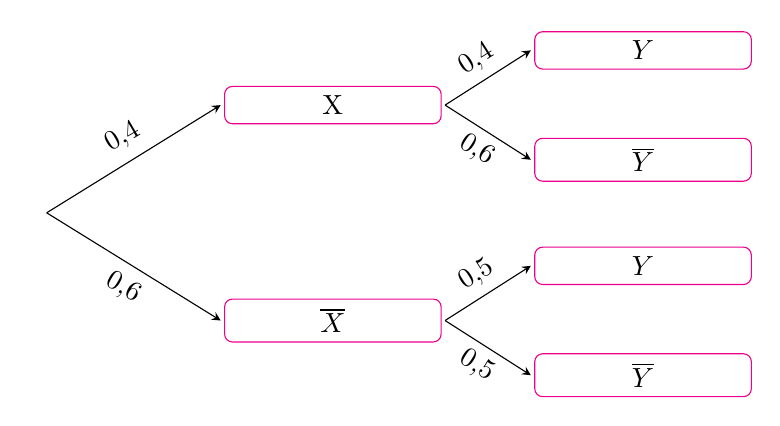
\begin{tikzpicture}
				\def\gocm{20}
				\def\gocn{10}
				\def\r{4}
				\tikzset{s/.style={outer sep=0.5 mm,draw=magenta,rectangle,minimum width=2.75cm,rounded corners=1mm}}
				\path(0,0)node(O){}++(\gocm:\r)node[s](A1){X}++(\gocn:\r)node[s](A2){$Y$};
				\path(A1)++({-\gocn}:\r)node[s](a2){$\overline{Y}$};
				\path(O)++(-\gocm:\r)node[s](B1){$\overline{X}$}++(\gocn:\r)node[s](B2){$Y$};
				\path(B1)++({-\gocn}:\r)node[s](b2){$\overline{Y}$};
				\foreach \x/\y in {
					O/A1,A1/A2,
					O/B1,B1/B2,
					A1/a2,
					B1/b2}
				\draw[-stealth](\x.east)--(\y.west);
				\path(O)--(A1.west)node[pos=0.5,above,sloped]{$0{,}4$}(O)--(B1.west)node[pos=0.5,below,sloped]{$0{,}6$}(B1.east)--(B2.west)node[pos=0.5,above,sloped]{$0{,}5$}(A1.east)--(A2.west)node[pos=0.5,above,sloped]{$0{,}4$}
				(A1.east)--(a2.west)node[pos=0.5,below,sloped]{$0{,}6$}
				(B1.east)--(b2.west)node[pos=0.5,below,sloped]{$0{,}5$};
				
			\end{tikzpicture}
			
		\end{center}
		Khi đó $\mathrm{P}(B)=\mathrm{P}(X\overline{Y})+\mathrm{P}(\overline{X}Y)=0{,}4\cdot 0{,}6+0{,}6\cdot 0{,}5=0{,}54$.
	}
\end{bt}

\begin{ex}%[2D6V2-4]
% nguon: Archive/SP_KhoLatex/SP_Bộ đề OTK12/SP_Data/2-B19-De2.tex #4315
%4
Một loại linh kiện do hai nhà máy số I, số II cùng sản xuất. Tỉ lệ phế phẩm của các nhà máy I, II lần lượt là $4\%$; $3\%$. Trong một lô linh kiện để lẫn lộn $80$ sản phẩm của nhà máy số I và $120$ sản phẩm của nhà máy số II. Một khách hàng lấy ngẫu nhiên một linh liện từ lô hàng đó. Xét các biến cố sau
\begin{itemize}
				\item $A$: \lq\lq Linh kiện lấy ra là linh kiện tốt\rq\rq.
				\item $B_1$: \lq\lq Linh kiện lấy ra là linh kiện từ nhà máy số I\rq\rq.
				\item $B_2$: \lq\lq Linh kiện lấy ra là linh kiện từ nhà máy số II\rq\rq.
\end{itemize}
\choiceTF
{\True $\mathrm{P}(B_1)=0{,}4$}
{\True $\mathrm{P}\left(A|B_2\right) =  0{,}97$}
{\True $\mathrm{P}(A) = 0{,}966$}
{Nếu linh kiện được lấy ra là linh kiện phế phẩm thì xác suất linh kiện đó do nhà máy II sản xuất là cao nhất}
\loigiai{
Theo đề bài, ta có
			\begin{listEX}[2]
				\item $\mathrm{P}(A|B_1) =1 - 0{,}04 = 0{,}96$.
				\item $\mathrm{P}\left(A|B_2\right) = 1-0{,}03 = 0{,}97$.
				\item $\mathrm{P}(B_1)=\dfrac{80}{200}=0{,}4$.
				\item $\mathrm{P}\left(B_2\right) = \dfrac{120}{200}=0{,}6$.
			\end{listEX}
			Khi đó áp dụng công thức xác suất toàn phần, ta có
			\[\mathrm{P}(A) = \mathrm{P}(A|B_1)\cdot \mathrm{P}(B_1) + \mathrm{P}\left(A|B_2\right)\cdot\mathrm{P}\left(B_2\right)=0{,}96\cdot 0{,}4 + 0{,}97\cdot 0{,}6=0{,}966.\]
			Ta có $\mathrm{P}\left(\overline{A}\right)=1-\mathrm{P}(A) = 0{,}034$.\\
			Áp dụng công thức Bayes, ta có
			\begin{itemize}
				\item $\mathrm{P}\left(B_1|\overline{A}\right)=\dfrac{\mathrm{P}\left(\overline{A}|B_1\right)\cdot \mathrm{P}(B_1)}{\mathrm{P}\left(\overline{A}\right)} = \dfrac{0{,}04\cdot 0{,}4}{0{,}034} = \dfrac{8}{17}\approx 0{,}048$.
				\item $\mathrm{P}\left(B_2|\overline{A}\right)=\dfrac{\mathrm{P}\left(\overline{A}|B_2\right)\cdot \mathrm{P}(B_2)}{\mathrm{P}\left(\overline{A}\right)} = \dfrac{0{,}03\cdot 0{,}6}{0{,}034} = \dfrac{8}{167}\approx 0{,}054$.
			\end{itemize}
			Vậy với điều kiện linh kiện lấy ra là linh kiện phế phẩm thì xác suất linh kiện đó do nhà máy I sản xuất là cao nhất.
%\begin{itemchoice}
%	\itemch \textbf{Đúng}. 
%	\itemch \textbf{Đúng}. 
%	\itemch \textbf{Đúng}.
%	\itemch \textbf{Sai}.
%\end{itemchoice}
}
\end{ex}

\begin{bt}%[2D6H2-2]
% nguon: Archive/SP_KhoLatex/SP_Bộ đề OTK12/SP_Data/2-B19-De2.tex #4317

	Một loại vaccine được tiêm ở địa phương X. Người có bệnh nền thì với xác suất $0{,}35$ có phản ứng phụ sau tiêm, người không có bệnh nền thì chỉ có phản ứng phụ sau tiêm với xác suất $0{,}16$. Chọn ngẫu nhiên một người được tiêm vaccine. Tính xác suất người này có phản ứng phụ, biết rằng tỉ lệ người có bệnh nền ở địa phương X là $18\%$. (Làm tròn đến hàng phần trăm).
	\shortans{$0{,}19$}
	\loigiai{
		Gọi $A$ là biến cố \lq\lq Người được chọn có bệnh nền\rq\rq\, và $B$ là biến cố \lq\lq Người này có phản ứng phụ sau tiêm\rq\rq.\\
		Ta có $\mathrm{P}(A)=0{,}18$; $\mathrm{P}(\overline{A})=0{,}82$.\\
		$\mathrm{P}(B\mid A)$ là xác suất để một người bệnh có phản ứng sau tiêm với điều kiện có bệnh nền, suy ra $\mathrm{P}(B\mid A)=0{,}35$.\\
		$\mathrm{P}(B\mid \overline{A})$ là xác suất để một người bệnh có phản ứng sau tiêm với điều kiện không có bệnh nền, suy ra $\mathrm{P}(B\mid \overline{A})=0{,}16$.\\
		Theo công thức xác suất toàn phần, ta được 
		$$\mathrm{P}(B)=\mathrm{P}(A)\cdot \mathrm{P}(B\mid A)+\mathrm{P}(\overline{A})\cdot \mathrm{P}(B\mid \overline{A})=0{,}18\cdot 0{,}35+0{,}82\cdot 0{,}16=\dfrac{971}{5\,000}\approx 0{,}19.$$
	}
\end{bt}

\begin{bt}%[2D6V2-3]
% nguon: Archive/SP_KhoLatex/SP_Bộ đề OTK12/SP_Data/2-B19-De2.tex #4318

Người ta điều tra thấy ở một địa phương nọ có $2\%$ tài xế sử dụng điện thoại di động khi lái xe. Trong các vụ tai nạn ở địa phương đó, người ta nhận thấy có $10\%$ là do tài xế có sử dụng điện thoại khi lái xe gây ra. Hỏi việc sử dụng điện thoại di động khi lái xe làm tăng xác suất gây tai nạn lên bao nhiêu lần?
\shortans{$5$}
\loigiai{
Gọi $ A $ là biến cố \lq\lq Tài xế sử dụng điện thoại di động khi lái xe\rq\rq\,và $ B $ là biến cố \lq\lq Địa phương có tai nạn\rq\rq.\\
Do có $ 2\% $ tài xế sử dụng điện thoại di động khi lái xe nên $ \mathrm{P}(A)=0{,}02 $.\\
Do trong các vụ tai nạn ở địa phương, có $ 10\% $ là do tài xế có sử dụng điện thoại khi lái xe nên $ \mathrm{P}(A|B)=0{,}1 $.
Xác suất gây tai nạn do tài xế sử dụng điện thoại di động khi lái xe là
$$ \mathrm{P}(B|A)= \dfrac{\mathrm{P}(B)\mathrm{P}(A|B)}{\mathrm{P}(A)}$$
Do đó $ \dfrac{\mathrm{P}(B|A)}{\mathrm{P}(B)}=\dfrac{\mathrm{P}(A|B)}{\mathrm{P}(A)}=\dfrac{0{,}1}{0{,}02}= 5$. Suy ra $ \mathrm{P}(B|A)=5\mathrm{P}(B) $.\\
Vậy việc sử dụng điện thoại di động khi lái xe làm tăng xác suất gây tai nạn lên $5$ lần.
}
\end{bt}

\begin{bt}%[2D6C2-4]
% nguon: Archive/SP_KhoLatex/SP_Bộ đề OTK12/SP_Data/2-B19-De2.tex #4319

Tỉ lệ người dân đã tiêm vắc xin phòng bệnh A ở một địa phương là $65\%$. Trong số những  người đã tiêm phòng, tỉ lệ mắc bệnh A là $5\%$ còn trong số những người chưa tiêm, tỉ lệ mắc bệnh A là $17\%$. Gặp ngẫu nhiên một người ở địa phương đó. Biết rằng người đó mắc bệnh X. Khi đó xác suất người đó không tiêm vắc xin phòng bệnh X có dạng $\dfrac{a}{b}$. Giá trị $b-a$ là?
\shortans{$65$}
\loigiai{
Gọi $A$ là biến cố \lq\lq người đó mắc bệnh $X$\rq\rq\,và $B$ là biến cố \lq\lq Gặp được người đã tiêm vắc xin phòng bệnh X\rq\rq.\\
Theo công thức xác suất toàn phần, ta có
\begin{eqnarray*}
	\mathrm{P}(A) & = &\mathrm{P}(B) \cdot \mathrm{P}(A \mid B)+\mathrm{P}(\overline{B}) \cdot \mathrm{P}(A \mid \overline{B}) \\
& = &0,65 \cdot 0{,}05+0{,}35 \cdot 0{,}17=0{,}092.
\end{eqnarray*}
Suy ra
\begin{eqnarray*}
\mathrm{P}(\overline{B} \mid A) & =& \dfrac{\mathrm{P}(A \overline{B})}{\mathrm{P}(A)}=\dfrac{\mathrm{P}(\overline{B}) \mathrm{P}(A \mid \overline{B})}{\mathrm{P}(A)} \\
& =& \dfrac{0,35 \cdot 0{,}17}{0{,}092}=\dfrac{119}{184}.
\end{eqnarray*}
Khi đó $a=119$ và $b=184$, suy ra $b-a=65$.
}
\end{bt}

\begin{ex}%[2D6H1-2]
% nguon: Archive/SP-4Phan-Dot3/Data/CD_2-OTHK2-De01.tex #4413
%[Dự án đè thi 4 phần đợt 3]%[Trần Xuân Hòa]
	Một công ty truyền thông đấu thầu $2$ dự án. Khả năng thắng thầu của dự án $1$ là $0{,}5$ và dự án $2$ là $0{,}6$. Khả năng thắng thầu của cả $2$ dự án là $0{,}4$. Gọi $A$, $B$ lần lượt là biến cố thắng thầu dự án $1$ và dự án $2$, khi đó
	\choiceTF
	{$A$ và $B$ là hai biến cố độc lập}
	{\True Xác suất công ty thắng thầu đúng $1$ dự án là $0{,}3$}
	{Biết công ty thắng thầu dự án $1$, xác suất công ty thắng thầu dự án $2$ là $0{,}4$}
	{Biết công ty không thắng thầu dự án $1$, xác suất công ty thắng thầu dự án $2$ là $0{,}8$}
	\loigiai{
		Ta có $\mathrm{P}(A)=0{,}5$; $\mathrm{P}(B)=0{,}6$; $\mathrm{P}(A B)=0{,}4$.
		\begin{itemchoice}
			\itemch $\mathrm{P}(A) \cdot \mathrm{P}(B)=0{,}5 \cdot 0{,}6=0{,}3 \neq \mathrm{P}(A B)$ nên $A$ và $B$ không là hai biến cố độc lập.
			\itemch 
			Xác suất công ty thắng thầu đúng 1 dự án là $\mathrm{P}(A)+\mathrm{P}(B)-2 \cdot \mathrm{P}(A B)=0{,}3$.
			\itemch 
			Biết công ty thắng thầu dự án 1, xác suất công ty thắng thầu dự án 2 là
			$$\mathrm{P}(B \mid A)=\dfrac{\mathrm{P}(A B)}{\mathrm{P}(A)}=0{,}8.$$
			\itemch 
			Biết công ty không thắng thầu dự án 1, xác suất công ty thắng thầu dự án 2 là
			$$\mathrm{P}(B \mid \overline{A})=\dfrac{\mathrm{P}(B \overline{A})}{\mathrm{P}(\overline{A})}=\dfrac{\mathrm{P}(B)-\mathrm{P}(A B)}{1-\mathrm{P}(A)}=0{,}4.$$
		\end{itemchoice}
	}
\end{ex}

\begin{bt}%[2D6C2-2]
% nguon: Archive/SP-4Phan-Dot3/Data/KNTT_2-OTHK2_De02.tex #4460
%[12-MH-1-MH2025]%[MH-2025, Mã/Tên TV biên soạn]
	Một công ty dược phẩm giới thiệu một dụng cụ để kiểm tra sớm bệnh sốt xuất huyết. Về báo cáo kiểm định chất lượng của sản phẩm, họ cho biết như sau: Số người được thử là $8\,000$, trong số đó có $1\,200$ người đã bị nhiễm bệnh sốt xuất huyết và có $6\,800$ người không bị nhiễm bệnh sốt xuất huyết. Nhưng khi kiểm tra lại bằng dụng cụ của công ty, trong $1\,200$ người đã bị nhiễm bệnh sốt xuất huyết, có $70 \%$ số người đó cho kết quả dương tính, còn lại cho kết quả âm tính. Trong $6\,800$ người không bị nhiễm bệnh sốt xuất huyết, có $5 \%$ số người đó cho kết quả dương tính, còn lại cho kết quả âm tính. Xác suất mà một bệnh nhân với kết quả kiểm tra dương tính là bị nhiễm bệnh sốt xuất huyết bằng bao nhiêu (viết kết quả dưới dạng số thập phân và làm tròn đến hàng phần trăm)?\par
	\shortans[]{$0{,}71$}
	\loigiai{
		\begin{itemize}
			\item Khi kiểm tra lại, trong $1\,200$ người đã bị nhiễm bệnh sốt xuất huyết, có $70 \%$ số người cho kết quả dương tính nên ta có $70 \% \cdot 1\,200=840$ (người).\\
			Khi đó, số người bị nhiễm bệnh sốt xuất huyết cho kết quả âm tính trong số $1\,200$ người đó là $1\,200-840=360$ (người).
			\item Khi kiểm tra lại, trong $6\,800$ người không bị nhiễm bệnh sốt xuất huyết, có $5 \%$ số người đó cho kết quả dương tính nên ta có là $5 \% \cdot 6\,800=340$ (người).\\
			Khi đó, số người không bị nhiễm bệnh sốt xuất huyết cho kết quả âm tính trong $6\,800$ người đó là $6\,800-340=6\,460$ (người).\\
			Từ đó, ta có bảng sau (đơn vị: người):
			\begin{center}
				\begin{tabular}{|c|c|c|c|}
					\hline \multirow{2}{*}{} & \begin{tabular}{c} 
						Số người \\
						nhiễm bệnh
					\end{tabular} & \begin{tabular}{c} 
						Số người không \\
						nhiễm bệnh
					\end{tabular} & Tổng số \\
					\cline {2 - 4 } & 1\,200 & 6\,800 & 8\,000 \\
					\hline Dương tính & 840 & 340 & 1\,180 \\
					\hline Âm tính & 360 & 6\,460 & 6\,820 \\
					\hline
				\end{tabular}
			\end{center}
			\item Xét các biến cố sau:
			\begin{itemize}
				\item $A$: \lq\lq Người được chọn ra trong số những người thử nghiệm là bị nhiễm bệnh sốt xuất huyết\rq\rq;
				\item $B$: \lq\lq Người được chọn ra trong số những người thử nghiệm là không bị nhiễm bệnh sốt xuất huyết\rq\rq;
				\item $C$: \lq\lq Người được chọn ra trong số những người thử nghiệm cho kết quả dương tính (khi kiểm tra lại)\rq\rq;
				\item $D$: \lq\lq Người được chọn ra trong số những người thử nghiệm cho kết quả âm tính (khi kiểm tra lại)\rq\rq.
			\end{itemize}
			Suy ra $\mathrm{P}(C)=\dfrac{1\,180}{8\,000}=\dfrac{59}{400}$ và $\mathrm{P}(AC)=\dfrac{840}{8\,000}=\dfrac{21}{200}$.\\
			Vậy $ \mathrm{P}(A\mid C)=\dfrac{21}{200}:\dfrac{59}{400}=\dfrac{42}{59}\approx 0{,}71$.
		\end{itemize}
	}
\end{bt}

\begin{ex}%[2D6H1-2]
% nguon: Archive/SP-4Phan-Dot3/Data/CTST_2-OTHK2-De05.tex #4540
%Câu 15
Một nhà máy có hai phân xưởng I và II. Phân xưởng I sản xuất $35\%$ số sản phẩm và phân xưởng II sản xuất $65\%$ số sản phẩm. Tỉ lệ sản phẩm bị lỗi của phân xưởng I là $2\% $ và của phân xưởng II là $3\% $. Kiểm tra ngẫu nhiên một sản phẩm của nhà máy.
\choiceTF
{\True Xác suất để sản phẩm được kiểm tra bị lỗi do phân xưởng II sản xuất là $\dfrac{39}{53}$}
{\True Xác suất để sản phẩm đó bị lỗi là $0{,}0265$}
{Xác suất để sản phẩm được kiểm tra bị lỗi do phân xưởng I sản xuất là $\dfrac{12}{53}$}
{Xác suất để sản phẩm đó không bị lỗi do phân xưởng I sản xuất là $0{,}89$}
\loigiai{
\begin{itemchoice}
\itemch Nếu sản phẩm được kiểm tra bị lỗi thì xác suất do phân xưởng II sản xuất là
\[\mathrm{P}\left(\overline B \mid  A\right)=1-\mathrm{P}\left(B\mid  A\right)=\dfrac{39}{53}.\]
\itemch Xác suất để sản phẩm đó bị lỗi là \[\mathrm{P}(A)=\mathrm{P}(B)\cdot \mathrm{P}\left(A\mid  B\right)+\mathrm{P}\left(\overline{B}\right)\mid \mathrm{P}\left(A\cdot\overline B\right)=0{,}35\cdot0{,}02+0{,}65\cdot0{,}03=\dfrac{53}{2000}=0{,}0265.\]
\itemch Nếu sản phẩm được kiểm tra bị lỗi thì xác suất do phân xưởng I sản xuất là
\[\mathrm{P}\left(B\mid A\right)=\dfrac{\mathrm{P}(B)\cdot \mathrm{P}\left(A\mid  B\right)}{\mathrm{P}(A)}=\dfrac{0{,}35\cdot0{,}02}{0{,}0265}=\dfrac{14}{53}.\]
\itemch Gọi $A$ là biến cố: \lq\lq Sản phẩm được kiểm tra bị lỗi \rq\rq.\\
Gọi $B$ là biến cố: \lq\lq Sản phẩm được kiểm tra do phân xưởng I sản xuất\rq\rq\, thì biến cố đối của $B$ là $\overline{B}$: \lq\lq Sản phẩm được kiểm tra do phân xưởng II sản xuất\rq\rq.\\
Khi đó, $\mathrm{P}(B)=0{,}35$; $\mathrm{P}\left(\overline B\right)=1-0{,}35=0{,}65$; $\mathrm{P}\left(A\mid  B\right)=0{,}02$; $\mathrm{P}\left(A\mid \overline B\right)=0{,}03$.\\
Vậy $\mathrm{P}\left(\overline A \mid  B\right)=1-\mathrm{P}(A\mid B)=0{,}98$.
\end{itemchoice}
}
\end{ex}

\begin{bt}%[2D6H2-2]
% nguon: Archive/SP-4Phan-Dot3/Data/CTST_2-OTHK2-De05.tex #4543

Mỗi bạn học sinh trong lớp của Minh lựa chọn một trong hai ngoại ngữ là tiếng Anh hoặc tiếng Nhật. Xác suất chọn tiếng Anh của mỗi bạn học sinh nữ là $0{,}6$ và của mỗi bạn học sinh nam là $0{,}7$. Lớp của Minh có $25$ bạn nữ và $20$ bạn nam. Chọn ra ngẫu nhiên một bạn trong lớp.Tính tổng xác suất của các biến cố (làm tròn đến hàng phần trăm).\\
A: \lq\lq Bạn được chọn là nam và học tiếng Nhật\rq\rq.\\
B: \lq\lq Bạn được chọn là nữ và học tiếng Anh\rq\rq .
\shortans{$0{,}47$}
\loigiai{ 
Gọi $A$ là biến cố \lq\lq Bạn được chọn là nữ\rq\rq  và $B$ là biến cố \lq\lq Bạn được chọn học tiếng Anh\rq\rq.\\
Ta có
$\mathrm{P}(Y\mid X)=0{,}6; \mathrm{P}(Y \mid \overline{X})=0{,}7$; $ \mathrm{P}(X)=\dfrac{5}{9}$.\\
Do đó $\mathrm{P}(\overline{X})=1-\mathrm{P}(X)=\dfrac{4}{9}$; $ \mathrm{P}(\overline{Y} \mid X)=1-\mathrm{P}(Y\mid X)=0{,}4$; \\ $\mathrm{P}(\overline{Y} \mid \overline{X})=1-\mathrm{P}(Y \mid \overline{X})=0{,}3$.\\
Ta có sơ đồ hình cây như sau
\begin{center}
	\begin{tikzpicture}
		\def\gocm{20}
		\def\gocn{10}
		\def\r{4}
		\tikzset{s/.style={outer sep=0.5 mm,draw=black,rectangle,minimum width=1.5cm,rounded corners=1mm}}
		\path(0,0)node(O){}++(\gocm:\r)node[s](A1){X}++(\gocn:\r)node[s](A2){$Y$};
		\path(A1)++({-\gocn}:\r)node[s](a2){$\overline{Y}$};
		\path(O)++(-\gocm:\r)node[s](B1){$\overline{X}$}++(\gocn:\r)node[s](B2){$Y$};
		\path(B1)++({-\gocn}:\r)node[s](b2){$\overline{Y}$};
		\foreach \x/\y in {O/A1,A1/A2,O/B1,B1/B2,A1/a2,B1/b2}
		\draw[-stealth](\x.east)--(\y.west);
		\path(O)--(A1.west)node[pos=0.5,above]{$\dfrac{5}{9}$}(O)--(B1.west)node[pos=0.5,below]{$\dfrac{4}{9}$}(B1.east)--(B2.west)node[pos=0.5,above,sloped]{$0{.}7$}(A1.east)--(A2.west)node[pos=0.5,above,sloped]{$0{.}6$}
		(A1.east)--(a2.west)node[pos=0.5,below,sloped]{$0{.}4$}
		(B1.east)--(b2.west)node[pos=0.5,below,sloped]{$0{.}3$};
	\end{tikzpicture}
\end{center}
Do $A=\overline{X}\cdot\overline{Y}$ nên $\mathrm{P}(\overline{X}\cdot\overline{Y})=\dfrac{4}{9}\cdot 0{,}3=\dfrac{2}{15}$.\\
Do $B=XY$ nên $\mathrm{P}(XY)=\dfrac{5}{9}\cdot 0{,}6=\dfrac{1}{3}$.\\
Vậy $\mathrm{P}(A)+\mathrm{P}(B)=\dfrac{2}{15}+\dfrac{1}{3}=\dfrac{7}{15}\approx0{,}47$.
}
\end{bt}

\begin{ex}%[2D6H2-2]
% nguon: Archive/SP-4Phan-Dot3/Data/CTST_2-OTHK2-De04.tex #4550

	Kết quả khảo sát những bệnh nhân bị tai nạn xe máy về mối liên hệ giữa việc đội mũ bảo hiểm và khả năng bị chấn thương vùng đầu cho thấy
	\begin{itemize}
		\item Tỉ lệ bệnh nhân bị chấn thương vùng đầu khi gặp tai nạn là $80 \%$;
		\item Tỉ lệ bệnh nhân đội mũ bảo hiểm đúng cách khi gặp tai nạn là $90 \%$;
		\item Tỉ lệ bệnh nhân đội mũ bảo hiểm đúng cách bị chấn thương vùng đầu là $18 \%$
	\end{itemize}
	Gọi A là biến cố: \lq\lq Bệnh nhân bị chấn thương vùng đầu khi gặp tai nạn\rq\rq\, và B là biến cố: \lq\lq Bệnh nhân đội mũ bảo hiểm đúng cách khi gặp tai nạn\rq\rq.
	\choiceTF
	{\True Xác suất để khi gặp tai nạn, bệnh nhân đội mũ bảo hiểm đúng cách và bị chấn thương vùng đầu là $0{,}144$}
	{Xác suất để khi gặp tai nạn, bệnh nhân không đội mũ bảo hiểm đúng cách và bị chấn thương vùng đầu khi gặp tai nạn là $0{,}65$}
	{\True Xác suất để khi gặp tai nạn, bệnh nhân không đội mũ bảo hiểm đúng cách biết bệnh nhân bị chấn thương vùng đầu là $0{,}82$}
	{\True Việc đội mũ bảo hiểm đúng cách sẽ làm giảm khả năng chấn thương vùng đầu xuống khoảng $4{,}6$ lần}
	\loigiai{
		\begin{itemchoice}
			\itemch Theo đề bài ta có $\mathrm{P}(A)=0{,}8; \mathrm{P}(B)=0{,}9; \mathrm{P}(B\mid A)=0{,}18$.\\
			Suy ra $\mathrm{P}(B\mid A)=\dfrac{\mathrm{P}(AB)}{\mathrm{P}(A)}\Rightarrow \mathrm{P}(AB)=\mathrm{P}(A)\cdot \mathrm{P}(B\mid A)=0{,}8\cdot 0{,}18=0{,}144$.
			\itemch Vì $A\overline{B}$ và $AB$ là hai biến cố xung khắc nên $A\overline{B}\cup AB=A$.\\
			Suy ra $\mathrm{P}\left(\overline{B}A\right)=\mathrm{P}(A)-\mathrm{P}(AB)=0{,}8-0{,}144=0{,}656$.
			\itemch Ta có  $\mathrm{P}\left(\overline{B}\mid A\right)=\dfrac{\mathrm{P}\left(\overline{B}A\right)}{\mathrm{P}(A)}=\dfrac{0{,}656}{0{,}8}=0{,}82$.
			\itemch Vì $\dfrac{\mathrm{P}\left(\overline{B}\mid A\right)}{\mathrm{P}(B\mid A)}=\dfrac{0{,}82}{0{,18}}\approx 4{,}6$ nên việc đội mũ bảo hiểm đúng cách sẽ làm giảm khả năng chấn thương vùng đầu xuống khoảng $4{,}6$ lần.
		\end{itemchoice}
	}
\end{ex}

\begin{bt}%[2D6V1-4]
% nguon: Archive/SP-4Phan-Dot3/Data/CTST_2-OTHK2-De04.tex #4553

	Một công ty đấu thầu hai dự án. Khả năng thắng thầu của các dự án $1$ là $0{,}4$ và dự án $2$ là $0{,}5$. Khả năng thắng thầu của cả hai dự án là $0{,}3$. Tính xác xuất để công ty thắng dự án $2$ biết công ty không thắng thầu dự án $1$ (làm tròn kết quả đến hàng phần trăm).
	\shortans{$0{,}33$}
	\loigiai{	
	Gọi $A$ là biến cố \lq\lq Công ty thắng thầu dự án 1\rq\rq, theo đề bài ta có $$\mathrm{P}(A)=0{,}4\Rightarrow \mathrm{P}\left(\overline{A}\right)=0{,}6.$$
	Gọi $B$ là biến cố: \lq\lq Công ty thắng thầu dự án 2\rq\rq, theo đề bài ta có $\mathrm{P}(B)=0{,}5$, và $\mathrm{P}(AB)=0{,}3$.\\
	Gọi $C$ là biến cố \lq\lq Công ty thắng dự án $2$ biết không thắng dự án $1$\rq\rq, ta có
	\[C=B|\overline{A}\Rightarrow \mathrm{P}(C)=\mathrm{P}\left(B|\overline{A}\right)=\dfrac{\mathrm{P}\left(\overline{A}B\right)}{\mathrm{P}\left(\overline{A}\right)}.
	\]
	Do $B=AB\cap \overline{A}B$ nên 
	\allowdisplaybreaks
\begin{eqnarray*}
&&\mathrm{P}(B)=\mathrm{P}\left(AB\cap \overline{A}B\right)=\mathrm{P}(AB)+\mathrm{P}\left(\overline{A}B\right)\\&\Rightarrow& \mathrm{P}\left(\overline{A}B\right)=\mathrm{P}(B)-\mathrm{P}(AB)=0{,}5-0{,}3=0{,}2.
\end{eqnarray*}
	Suy ra
	\[\mathrm{P}(C)=\mathrm{P}\left(B|\overline{A}\right)=\dfrac{\mathrm{P}\left(\overline{A}B\right)}{\mathrm{P}\left(\overline{A}\right)}=\dfrac{0{,}2}{0{,}6}=\dfrac{1}{3} \approx 0{,}33.
	\]
	}
\end{bt}

\begin{ex}%[2D6V2-4]
% nguon: Archive/SP-4Phan-Dot3/Data/CTST_2-OTHK2-De03.tex #4565

	Một công ty dược phẩm giới thiệu một dụng cụ kiểm tra sớm bệnh sốt xuất huyết. Về kiểm định chất lượng của sản phẩm, họ cho biết như sau: Số người được thử là $10\,000$ người, trong số đó có $2\,000$ người đã bị nhiễm bệnh sốt xuất huyết và có $8\,000$ người không bị nhiễm bệnh sốt xuất huyết. Khi thử bằng dụng cụ của công ty, trong $2\,000$ người đã bị nhiễm bệnh sốt xuất huyết, có $75\%$ số người đó cho kết quả dương tính, còn lại cho kết quả âm tính. Mặt khác, trong $8\,000$ người không bị nhiễm bệnh sốt xuất huyết, có $5\%$ số người đó cho kết quả dương tính, còn lại cho kết quả âm tính khi kiểm tra. Chọn ngẫu nhiên một người trong số những người thử nghiệm.\\
	Gọi $A$ là biến cố \lq\lq Người được chọn nhiễm sốt xuất huyết\rq\rq.\\
	Gọi $B$ là biến cố \lq\lq Người được chọn âm tính với dụng cụ thử\rq\rq.\\
	\choiceTF[t]
	{$\mathrm{P}(A)=\dfrac{2\,000}{10\,000}=0{,}4$}
	{\True $\mathrm{P}(B\mid A)=0{,}25$}
	{Xác suất để người được chọn âm tính với dụng cụ là $0{,}62$}
	{\True Biết rằng người đó có kết quả thử nghiệm âm tính, xác suất để người được chọn ra bị nhiễm bệnh sốt xuất huyết bằng $0{,}062$ (kết quả làm tròn kết quả đến hàng phần nghìn)}
	\loigiai{
		\begin{itemchoice}
			\itemch Sai. $\mathrm{P}(A)=\dfrac{2\,000}{10\,000}=0{,}2$ và $\mathrm{P}(\overline{A})=\dfrac{8\,000}{10\,000}=0{,}8$.
			\itemch Đúng. $\mathrm{P}(B\mid A)=0{,}25$ và $\mathrm{P}(B\mid \overline{A})=0{,}95$.
			\itemch Sai. Xác suất để người được chọn âm tính với dụng cụ là $$\mathrm{P}(B)=\mathrm{P}(A)\cdot \mathrm{P}(B|A)+\mathrm{P}({\overline{A}})\cdot \mathrm{P}(B|\overline{A})=0{,}81$$
			\itemch Đúng. Biết rằng người đó có kết quả thử nghiệm âm tính, xác suất để người được chọn ra bị nhiễm bệnh sốt xuất huyết bằng $0{,}062$ (kết quả làm tròn kết quả đến hàng phần nghìn)
		\end{itemchoice}
	}
\end{ex}

\begin{ex}%[2D6H2-2]
% nguon: Archive/SP-4Phan-Dot3/Data/CTST_2-OTHK2-De02.tex #4576

Kết quả khảo sát về mối liên hệ giữa việc mang khẩu trang đúng cách và khả năng nhiễm bệnh của những người đến bệnh viện cho thấy
	\begin{itemize}
		\item Tỉ lệ người bị nhiễm bệnh khi đến bệnh viện là $70\%$;
		\item Tỉ lệ người mang khẩu trang đúng cách khi đến bệnh viện là $85\%$;
		\item Tỉ lệ người mang khẩu trang đúng cách nhưng vẫn bị nhiễm bệnh là $15\%$.
	\end{itemize}
Gọi $A$ là biến cố: \lq\lq Người đó bị nhiễm bệnh khi đến bệnh viện\rq\rq\, và $B$ là biến cố: \lq\lq Người đó mang khẩu trang đúng cách khi đến bệnh viện\rq\rq.
	\choiceTF
	{\True Xác suất để khi đến bệnh viện, người đó vừa mang khẩu trang đúng cách vừa bị nhiễm bệnh là $10{,}5\%$}
	{Xác suất để khi đến bệnh viện, người đó không mang khẩu trang đúng cách nhưng vẫn bị nhiễm bệnh là $5{,}95\%$}
	{\True Xác suất để khi biết người đó bị nhiễm bệnh, người đó đã không mang khẩu trang đúng cách là $85\%$}
	{Tỷ lệ giảm khả năng nhiễm bệnh nếu mang khẩu trang đúng cách là $5$ lần}
	\loigiai{
	Ta có $\mathrm{P}(A) = 0{,}7$ (tỉ lệ người bị nhiễm bệnh);\\
	$\mathrm{P}(B) = 0{,}85$ (tỉ lệ người mang khẩu trang đúng cách);\\
	$\mathrm{P}(B\mid A) = 0{,}15$ (tỉ lệ người mang khẩu trang đúng cách nhưng vẫn bị nhiễm bệnh).
	\begin{itemchoice}
		\itemch {\bf{Đúng}}.\\
		Ta có
		\allowdisplaybreaks
		\begin{eqnarray*}
			\mathrm{P}(AB)&=&\mathrm{P}(A) \cdot \mathrm{P}(B\mid A)
			\\
			&=&0{,}7 \cdot 0{,}15 = 0{,}105.
		\end{eqnarray*}
	Vậy xác suất để khi đến bệnh viện, người đó vừa mang khẩu trang đúng cách vừa bị nhiễm bệnh là $0{,}105$.
		\itemch {\bf{Sai}}.\\
		Vì $A \overline{B}$ và $AB$ là hai biến cố xung khắc, nên ta có
			\[\mathrm{P}(A) = \mathrm{P}(AB) + \mathrm{P}\left(A\overline{B}\right).\]
			Suy ra \[\mathrm{P}\left(A\overline{B}\right) = \mathrm{P}(A) - \mathrm{P}(AB) = 0{,}7 - 0{,}105 = 0{,}595.\]
			Vậy xác suất để khi đến bệnh viện, người đó không mang khẩu trang đúng cách nhưng vẫn bị nhiễm bệnh là $0{,}595$.
		\itemch {\bf{Đúng}}.\\
		Ta có
		\allowdisplaybreaks
		\begin{eqnarray*}
			\mathrm{P}\left(\overline{B}\mid A\right)& =& \dfrac{P\left(A\overline{B}\right)}{P(A)}
			\\
			&=&\dfrac{0{,}595}{0{,}7} \approx 0{,}85.
		\end{eqnarray*}
	Vậy xác suất để khi biết người đó bị nhiễm bệnh, người đó đã không mang khẩu trang đúng cách là $0{,}85$.
		\itemch {\bf{Sai}}.\\
		Ta có $\dfrac{\mathrm{P}\left(\overline{B}\mid A\right)}{\mathrm{P}(B\mid A)} = \dfrac{0{,}85}{0{,}15} \approx 5{,}67 $.\\
		Vậy việc mang khẩu trang đúng cách sẽ làm giảm khả năng nhiễm bệnh khoảng $5{,}67$ lần.
	\end{itemchoice}
}
\end{ex}

\begin{bt}%[2D6V2-3]
% nguon: Archive/SP-4Phan-Dot3/Data/CTST_2-OTHK2-De02.tex #4580

Ở một thành phố, người ta điều tra thấy rằng có \(1\%\) số người đi bộ thường xuyên sử dụng tai nghe khi qua đường. Trong các vụ tai nạn ở thành phố, người ta nhận thấy \(8\%\) là do người đi bộ có sử dụng tai nghe khi qua đường gây ra. Hỏi việc sử dụng tai nghe khi qua đường làm tăng xác suất gây tai nạn lên bao nhiêu lần?
\shortans[oly]{$8$}
	\loigiai{
		Gọi
		\begin{itemize}
			\item $A\colon$ \lq\lq Người đi bộ sử dụng tai nghe khi qua đường\rq\rq.
			\item $B\colon$ \lq\lq Có tai nạn xảy ra ở thành phố\rq\rq.
	\end{itemize}
Theo đề bài
	\begin{itemize}
		\item Có $1\%$ người đi bộ sử dụng tai nghe khi qua đường, nên $\mathrm{P}(A) = 0{,}01$.
		\item Trong các vụ tai nạn, có $8\%$ là do người đi bộ sử dụng tai nghe khi qua đường gây ra, nên $\mathrm{P}(A\mid B) = 0{,}08$.
	\end{itemize}
Ta cần tính $\dfrac{\mathrm{P}(B\mid A)}{\mathrm{P}(B)}$ để xem việc sử dụng tai nghe khi qua đường làm tăng xác suất gây tai nạn lên bao nhiêu lần.\\
Sử dụng định lý Bayes
	\[\mathrm{P}(B\mid A) = \dfrac{\mathrm{P}(B) \cdot \mathrm{P}(A\mid B)}{\mathrm{P}(A)}.\]
Vì vậy
	\[\dfrac{\mathrm{P}(B\mid A)}{\mathrm{P}(B)} = \dfrac{\mathrm{P}(A\mid B)}{\mathrm{P}(A)} = \dfrac{0{,}08}{0{,}01} = 8.\]
Việc sử dụng tai nghe khi qua đường làm tăng xác suất gây tai nạn lên $8$ lần.}
\end{bt}
